\documentclass[edeposit,tocnosub,noragright,centerchapter,fullpagesingle,12pt]{uiuc_csthesis21}

\makeatletter

\usepackage{setspace}  % Useful for single, 1.5, and double spacing
\usepackage[numbers, sort]{natbib}  % Useful for formatting reference section
\usepackage{url}  % Useful for URLs
\usepackage{hyperref}  % Another package useful for URLs

\usepackage{lscape}  % Useful for wide tables or figures.
% Following command definition is from Stack Exchange: https://tex.stackexchange.com/questions/278113/single-landscape-page-with-page-number-at-the-bottom
% It adds *rotated* page numbers to the bottom of landscaped pages to meet the Graduate College standards (see page 7 here: https://grad.illinois.edu/files/pdfs/thesis-sample-chapter-straight-numbering.pdf)
\def\fillandplacepagenumber{
	\par
	\pagestyle{empty}
	\vbox to 0pt{\vss}
	\vfill
	\vbox to 0pt{
		\baselineskip 0pt
		\hbox to \linewidth{\hss}
		\baselineskip\footskip
		\hbox to \linewidth{\hfil\thepage\hfil}\vss
	}
}

%%%%%%%%%%%%%%%%%%%%%%%%%%%%%%%%%%%%%%%%%%%%%%%%%%%%%%%%%%%%%%%%%%%%%%%%%%%%%%%

\usepackage[utf8]{inputenc}
\usepackage[inference]{semantic}
%\usepackage[english]{babel}
\usepackage{csquotes}
\usepackage{pifont}
\usepackage{stmaryrd}
\usepackage{microtype}
\usepackage{amsmath,amsthm,amssymb}
%\usepackage[bookmarksdepth=3,linktoc=all,colorlinks=true,urlcolor=blue,linkcolor=blue,citecolor=blue]{hyperref}
%%\usepackage[style=ieee]{biblatex}
\usepackage[inline]{enumitem}
\usepackage{dirtytalk}
\usepackage{graphicx}
\usepackage{wrapfig}
\usepackage{subcaption}
\usepackage{listings}
\usepackage{xcolor}
\usepackage{longtable}
\usepackage{tabularx}
\usepackage{mathtools}
\usepackage{varwidth}
\usepackage{proof}
\usepackage[bottom]{footmisc}
\usepackage[bbgreekl]{mathbbol}

%%%%%%%%%%%%%%%%%%%%%%%%%%%%%%%%%%%%%%%%%%%%%%%%%%%%%%%%%%%%%%%%%%%%%%%%%%%%%%%
% TABLE PACKAGES
%
\usepackage{booktabs}  % Useful for high quality tables (e.g., you can replace \hrule with \toprule, \midrule, and \bottomrule).
%\usepackage{multicol}
%\usepackage{multirow}
%%%%%%%%%%%%%%%%%%%%%%%%%%%%%%%%%%%%%%%%%%%%%%%%%%%%%%%%%%%%%%%%%%%%%%%%%%%%%%%
% MATH PACKAGES (Comment out this section if unnecessary for your dissertation)
%
\usepackage{amsfonts}
\usepackage{amsmath}
\usepackage{amssymb}
\usepackage{amstext}
\usepackage{amsthm}
\usepackage[capitalize]{cleveref}


\DeclareSymbolFontAlphabet{\mathbbm}{bbold}
\DeclareSymbolFontAlphabet{\mathbb}{AMSb}%

% Change numbering of definitions, lemmas, theorems, etc to meet the Graduate College standards
\theoremstyle{definition}
\newtheorem{definition}{Definition}[chapter]
\newtheorem{lemma}{Lemma}[chapter]
\newtheorem{theorem}{Theorem}[chapter]
\newtheorem{corollary}{Corollary}[chapter]
\newtheorem{conjecture}{Conjecture}[chapter]
\newtheorem{remark}{Remark}[chapter]

\renewcommand{\qedsymbol}{QED.}  % Change symbol at end of proofs to meet the Graduate College standard
%%%%%%%%%%%%%%%%%%%%%%%%%%%%%%%%%%%%%%%%%%%%%%%%%%%%%%%%%%%%%%%%%%%%%%%%%%%%%%%
% ALGORITHM AND CODE PACKAGES (Comment out this section if unnecessary for your dissertation)
%
\usepackage{listings}  % Useful for formatting code blocks, see here for further information about formatting code: https://en.wikibooks.org/wiki/LaTeX/Source_Code_Listings
\usepackage[ruled]{algorithm2e}  % Useful for formatting algorithms (pseudocode)
\numberwithin{algocf}{chapter}     % Change numbering of algorithms to meet the Graduate College standards

\definecolor{greybackground}{rgb}{0.95,0.95,0.92}
\definecolor{codegreen}{rgb}{0,0.6,0}
\definecolor{codegray}{rgb}{0.5,0.5,0.5}
\definecolor{codepurple}{rgb}{0.58,0,0.82}

% K lst definition
\lstdefinestyle{ksty}{
  keywordstyle=\color{magenta},
  basicstyle=\ttfamily\small,
  commentstyle=\color{codepurple},
  backgroundcolor=\color{greybackground},
  framerule=0pt
}
\lstdefinestyle{inlineksty}{
  basicstyle=\ttfamily\small
}
\lstdefinelanguage{k}{
  morekeywords={rule,configuration,=>,syntax,multiplicity,type,module,endmodule,import,imports, left,strict,seqstrict,bracket,structural,requires},
  morecomment=[l]{//},
  morecomment=[s]{/*}{*/}
}

% MediK lst definition
\lstdefinestyle{mediksty}{
  keywordstyle=\color{magenta},
  basicstyle=\ttfamily\small,
  commentstyle=\color{codepurple},
  backgroundcolor=\color{greybackground},
  framerule=0pt
}
\lstdefinestyle{inlinemediksty}{
  basicstyle=\ttfamily\small,
}
\lstdefinelanguage{medik}{
  morekeywords={either, or, machine, interface, vars, state, entry, on, do, goto, receives, ~>, =>},
  morecomment=[l]{//},
  morecomment=[s]{/*}{*/}
}

%Imp lst definition
\lstdefinestyle{impsty}{
  keywordstyle=\color{magenta},
  basicstyle=\ttfamily\small,
  backgroundcolor=\color{greybackground},
  commentstyle=\color{codepurple},
  framerule=0pt
}
\lstdefinelanguage{imp}{
  morekeywords={if, while, var}
  morecomment=[l]{//},
  morecomment=[s]{/*}{*/}
}

\newcommand{\inlinemedik}[1]{\lstinline[style=inlinemediksty,language=medik]{#1}}
\newcommand{\inlinek}[1]{\lstinline[style=inlineksty,language=k]{#1}}
\newcommand{\inlineimp}[1]{\lstinline[style=impsty,language=imp]{#1}}
\newcommand{\inlinekmath}[1]{\lstinline[mathescape,style=inlineksty,language=k,keepspaces]!#1!}
\newcommand{\inlinemedikmath}[1]{\lstinline[mathescape,style=inlinemediksty,language=medik]!#1!}
\newcommand{\inlinemedikimp}[1]{\lstinline[mathescape,style=inlineimpsty,language=imp]!#1!}
\lstset{ literate={~}{{\raisebox{0.5ex}{\texttildelow}}}{1} }
\lstset{captionpos=b,escapeinside={@}{@}}
\providecommand*{\lstnumberautorefname}{Line}
\def\boxit#1{%
  \smash{\color{red}\fboxrule=1pt\relax\fboxsep=2pt\relax%
  \llap{\rlap{\fbox{\vphantom{0}\makebox[#1]{}}}~}}\ignorespaces
}

\graphicspath{{./figures}}
\newcommand{\frontend}{\emph{frontend}}
\newcommand{\BPG}{BPG}
\newcommand{\BPGs}{BPGs}
\newcommand{\CGS}{CGS}
\newcommand{\CGSs}{CGSs}
\newcommand{\HCP}{HCP}
\newcommand{\HCPs}{HCPs}
\newcommand{\ED}{ED}
\newcommand{\EDs}{EDs}
\newcommand{\CDSS}{CDSS}
\newcommand{\CDSSs}{CDSSs}
\newcommand{\BPGLogic}{knowledge-base}
\newcommand{\K}{\mathbb{K}}
\newcommand{\MediK}{\text{Medi}\K{}}
\newcommand{\FSM}{\emph{FSM}}
\newcommand{\FSMs}{\emph{FSMs}}
\newcommand{\Var}{\text{Var}}
\newcommand{\LHS}{\emph{\text{LHS}}}
\newcommand{\RHS}{\emph{\text{RHS}}}
\renewcommand{\phi}{\varphi}
\newcommand{\GUI}{GUI}
\newcommand{\UI}{UI}
\newcommand{\UIs}{UIs}
\newcommand{\GUIs}{GUIs}
\newcommand{\PME}{PME}
\newcommand{\PMEs}{PMEs}
\newcommand{\CIG}{CIG}
\newcommand{\CIGs}{CIGs}
\newcommand{\EHRs}{EHRs}
\newcommand{\ACLS}{ACLS}
\newcommand{\CPR}{CPR}
\newcommand{\CISs}{CISs}
\newcommand{\RTSs}{RTSs}
\newcommand{\ASMs}{ASMs}
\newcommand{\DSL}{\text{DSL}}
\newcommand{\DSLs}{\text{DSLs}}
\newcommand{\IT}{IT}
\newcommand{\EHR}{EHR}
\newcommand{\ONC}{ONC}
\newcommand{\NAM}{NAM}
\newcommand{\BNF}{BNF}
\newcommand{\MLM}{\text{MLM}}
\newcommand{\MLMs}{\text{MLMs}}
\newcommand{\GLIF}{\text{GLIF}}
\newcommand{\GEODECM}{\text{GEODE-CM}}
\newcommand{\PCAPE}{\text{P-CAPE}}
\newcommand{\DEGEL}{\text{DeGeL}}
\newcommand{\GLARE}{\text{GLARE}}
\newcommand{\GPROVE}{\text{GPROVE}}
\newcommand{\GOSPEL}{\text{GOSpeL}}
\newcommand{\GEE}{\text{GEE}}
\newcommand{\AAP}{\text{AAP}}
\newcommand{\NHS}{\text{NHS}}
\newcommand{\GP}{\text{GP}}
\newcommand{\GPs}{\text{GPs}}
\newcommand{\SAGE}{\text{SAGE}}
\newcommand{\MPS}{\text{MPS}}
\newcommand{\PC}{\text{PC}}
\newcommand{\PlanSet}{\text{PlanSet}}
\newcommand{\PatientSet}{\text{PatientSet}}
\newcommand{\ConditionSet}{\text{ConditionSet}}
\newcommand{\FinalStateSet}{\text{FinalStateSet}}
\newcommand{\Considered}{\text{Considered}}
\newcommand{\filter}{\text{filter}}
\newcommand{\possible}{\text{possible}}

% Convenience Commands
\newcommand{\cmark}{\text{\ding{51}}}
\newcommand{\xmark}{\text{\ding{55}}}
\newcommand{\greencheck}{{\color{green}\cmark}}
\newcommand{\redcross}{{\color{red}\xmark}}
\newcommand{\cancelcheck}{\bcancel{\cmark}}
\newcommand{\stress}[1]{\underline{\emph{#1}}}

% Scheduling Commands
\newcommand{\Machine}{\mathcal{M}}
\newcommand{\Instance}{\mathcal{I}}
\newcommand{\scheduled}{\textit{scheduled}}
\newcommand{\enabled}{\textit{enabled}}
\newcommand{\epoch}{\textit{epoch}}

% Logic-Related
\newcommand{\antecedent}[1]{\text{antecedent}\left(#1\right)}
\newcommand{\consequent}[1]{\text{consequent}\left(#1\right)}



%%%%%%%%%%%%%%%%%%%%%%%%%%%%%%%%%%%%%%%%%%%%%%%%%%%%%%%%%%%%%%%%%%%%%%%%%%%%%%%
% COVERPAGE
%

% Uncomment the appropriate one of the following four lines:
%\msthesis
\phdthesis
%\otherdoctorate[abbrev]{Title of Degree}
%\othermasters[abbrev]{Title of Degree}

\title{A Semantics-First Approach to Safe Guidelines-based Clinical Decision Support}
\author{Manasvi Saxena}
\department{Computer Science}
\degreeyear{2024}

% Advisor name is required for
% - doctoral students for the ProQuest abstract
% - master's students who do not have a master's committee
\advisor{Professor Grigore Ro\c{s}u}

% Uncomment the \committee command for
% - all doctoral students
% - master's students who have a master's committee
\committee{Professor Grigore Ro\c{s}u, Chair\\
        Professor Jose Meseguer \\
        Professor Lui Sha \\
        Doctor Serdar Tasiran, Amazon Web Services (AWS)} % etc.

\begin{document}

%%%%%%%%%%%%%%%%%%%%%%%%%%%%%%%%%%%%%%%%%%%%%%%%%%%%%%%%%%%%%%%%%%%%%%%%%%%%%%%
% COPYRIGHT
%
%\copyrightpage
%\blankpage

%%%%%%%%%%%%%%%%%%%%%%%%%%%%%%%%%%%%%%%%%%%%%%%%%%%%%%%%%%%%%%%%%%%%%%%%%%%%%%%
% TITLE
%
\maketitle

%\raggedright
\parindent 1em%

\frontmatter

%%%%%%%%%%%%%%%%%%%%%%%%%%%%%%%%%%%%%%%%%%%%%%%%%%%%%%%%%%%%%%%%%%%%%%%%%%%%%%%
% ABSTRACT
%
\begin{abstract}
  Preventable medical errors (PMEs), characterized by misdiagnosis or mistreatment,
  pose a significant challenge in healthcare.
  In the United States, PMEs were estimated to have caused between
  44,000 and 98,000 deaths in 1997,
  rising to more than 250,000 in 2013. Additionally, the
  financial burden of PMEs to the U.S. economy in 2008 was estimated at \$19.5 billion.

  One strategy to reduce PMEs in medicine is through the use of
  clinical best practice guidelines (BPGs). BPGs are systematically developed,
  evidence-based statements published by medical institutions and associations
  that standardize diagnosis and treatment for various clinical scenarios.
  BPG-conformance has been linked with reduced rates of PMEs, but,
  following BPGs in practice can be challenging.
  Computerized Decision Support Systems (CDSSs) aim to improve conformance
  by encoding medical knowledge in BPGs and providing HCPs with
  situation-specific, guideline-conformant advice.
  Growing evidence suggests that
  effective CDSSs can reduce PMEs by boosting adherence to best practice guidelines.

  This work presents a semantics-first approach to implementing safe clinical
  decision support systems. By semantics-first,
  we mean that
  \begin{enumerate*}[label=\roman*]
    \item semantics of medical knowledge is
  accurately captured in the CDSS, and,
  \item the semantics of the programming language
    used to encode medical knowledge is formally defined.
  \end{enumerate*}
  At the core of our approach is \MediK{}: a novel domain specific language
  for expressing best practice guidelines that emphasizes comprehensibility
  to HCPs, enabling them to validate the accuracy of medical knowledge in its
  programs. \MediK{} has a complete, executable formal semantics in the \K{} Framework,
  from which all execution and analysis tools are derived in a
  correct-by-construction manner.

  To evaluate our approach, we collaborated with a major pediatric hospital
  to develop a complex real-world CDSS for the screening and management of
  Sepsis in pediatric cases, and validated that it satisfies desired safety properties.
  We outline how our approach improves upon the existing state-of-art,
  optimizations to address domain-specific needs of healthcare practitioners,
  and discuss challenges for future work.
\end{abstract}

%%%%%%%%%%%%%%%%%%%%%%%%%%%%%%%%%%%%%%%%%%%%%%%%%%%%%%%%%%%%%%%%%%%%%%%%%%%%%%%
% DEDICATION (Uncomment this section if desired)
%
\begin{dedication}
To my parents and my sister,
for their love and unconditional support,
and for always believing in me, even when challenges ensued.
\end{dedication}

%%%%%%%%%%%%%%%%%%%%%%%%%%%%%%%%%%%%%%%%%%%%%%%%%%%%%%%%%%%%%%%%%%%%%%%%%%%%%%%
% ACKNOWLEDGMENTS
%
\begin{acknowledgments}
While my journey at the University of Illinois has been long and challenging,
  I have been fortunate to have had the support of several wonderful people.

  First, I would like to thank my advisor, Prof. Grigore Ro\c{s}u,
  for his unwavering support and encouragement ever since I joined his research group as an undergraduate in the summer of 2014.

I am also extremely grateful to Prof. Lui Sha,
  with whom I have worked closely during the latter half of my PhD.
  His guidance, insights, and encouragement have been invaluable.
  I’d also like to thank him for his financial support, which enabled me to further develop my ideas.

I would like to express my sincere thanks to
  Dr. Serdar Tasiran for his mentorship during two summer internships at AWS’s S3 Automated Reasoning Group (S3-ARG),
  where I also had the opportunity to collaborate with Dr. Ankush Desai and Dr. Dongyun Jin,
  from whom I learned a great deal.
  I am also thankful to Serdar for impressing upon me the importance of
  effectively presenting ideas--a skill I have worked hard to improve based on his advice.

I am grateful to Prof. Jose Meseguer for his valuable insights
into implementing industrial-scale systems for use by non-experts in computer science.

I would also like to thank Prof. Rosu, Prof. Meseguer, Prof. Sha,
  and Dr. Tasiran for serving on my doctoral committee and for their time, expertise, and feedback.

I’d like to thank my labmates,
  both current and former, with whom I’ve had the pleasure of working with and learning from.
  Thank you, Daejun, Yi, Owolabi, Lucas, Xiaohong, Mircea, Nishant, Shuang, and Simon.
  A special shout-out goes to Nishant and Shuang for their companionship outside the lab,
  and to old friends Amulya, Neelabh, Rajiv, Dhruv, Balaji, and Aditya for always keeping me in the loop,
  even when I was too busy to respond.

I would like to extend my deepest gratitude to my family,
  both in the U.S. and in India.
I'd like to thank my uncle, aunt, and cousins, who always made sure I had a home away from home.
And to my parents and sister--thank you for the unconditional love, support, and unwavering belief in me, even during my moments of doubt.

\end{acknowledgments}

%%%%%%%%%%%%%%%%%%%%%%%%%%%%%%%%%%%%%%%%%%%%%%%%%%%%%%%%%%%%%%%%%%%%%%%%%%%%%%%
% TABLE OF CONTENTS
%
\tableofcontents

\mainmatter

%%%%%%%%%%%%%%%%%%%%%%%%%%%%%%%%%%%%%%%%%%%%%%%%%%%%%%%%%%%%%%%%%%%%%%%%%%%%%%%
% INSERT REAL CONTENT HERE

\section{Introduction}

Preventable Medical Errors (\PMEs{}) characterized by
incorrect intended treatment, or incorrect executions of intended
treatment present a significant challenge in Healthcare
\cite{RodziewiczStatsPearls18}. According to a seminal report on the subject
\cite{DonaldsonBook00}, in 1997,
between 44,000 and 98,000 deaths were estimated to have been caused by \PMEs{} in
the United States alone. A more recent study analyzed data from the eight-year
period between 2000 and 2008, and estimated that in 2013, the number of deaths
caused by \PMEs{} was more than 250,000, making \PMEs{} the third-leading
cause of death in the United States \cite{MakaryBMJ16}.
The adverse effects of \PMEs{} extend beyond patient outcomes.
One study estimated the financial burden of \PMEs{} to the United States to be
19.5 billion dollars in 2008 \cite{AndelJHCF12}. According to the authors of
\cite{RodziewiczStatsPearls18}, \PMEs{} caused psychological effects such
as anger and guilt in healthcare providers (\HCPs{}), adversely impacting their mental
health.

One strategy to mitigate \PMEs{} is to utilize evidence-based statements
published by hospital and medical associations that codify recommended
interventions for various clinical scenarios called Best Practice Guidelines (\BPGs{})
\cite{field1990clinical}. High quality guidelines are routinely updated to account for
 results from clinical trials and advances in medicine, and make the latest
 diagnosis and treatment information accessible to providers \cite{SteinbergNAP11}.

While \BPGs{} have the potential to reduce medical errors, their effectiveness hinges
on the adherence of healthcare providers to them.
For example, consider Advanced Cardiac Life Support (\ACLS{}): a \BPG{} published
by the American Heart Association (AHA) for management
of a life threatening condition called in-hospital cardiac arrest (IHCA) \cite{AHAGuidelineAdult, AHAGuidelinePed}. Studies suggest that management
of IHCA in 30\% of adult, and 17\% of pediatric cases deviates from the
AHA-prescribed \BPG, resulting in worse patient outcomes \cite{Ornato2012DeviationAdult,Wolfe2020DeviationPediatric,
Crowley2020DeviationAdult,Honarmand2018Adherence,Mcevoy2014Adherence}.

\begin{wrapfigure}{l}{0.5\textwidth}
  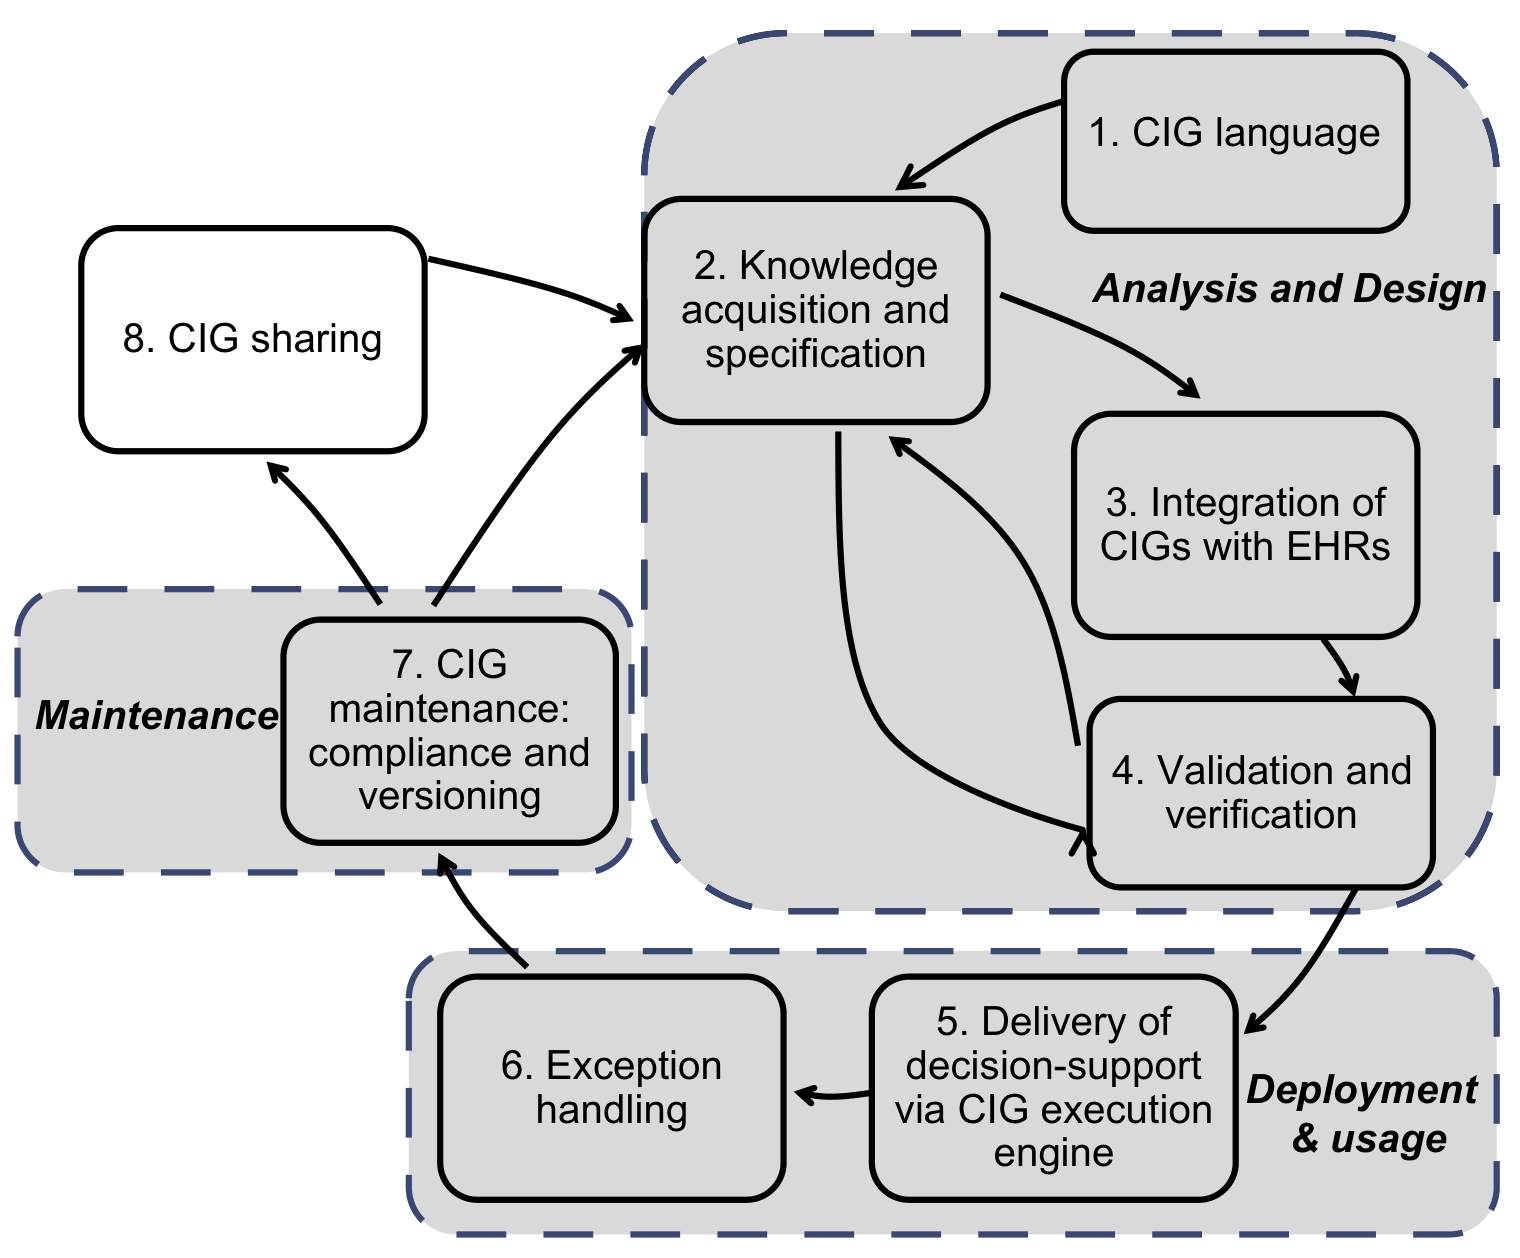
\includegraphics[width=\textwidth]{cpg-topics}
  \caption{\CDSSs{} Research Themes}\label{fig:cpg-research-topics}
\end{wrapfigure}

While \BPG{}-adherence is difficult to achieve in
practice \cite{RandJAMA99,DavisCMAJ97},
integrating \BPGs{} with existing patient care-flow,
and making them readily-accessible when required can improve adherence \cite{WoolfBMJ99}.
To this end, hospitals commission computerized Decision Support Systems (\CDSSs{})
that codify \BPGs{} and support \HCPs{} with situation-specific advice.
Such systems have been shown to improve \BPG{}-adherence \cite{GargJAMA06,KawamotoBMJ05}, and evidence from multi-center clinical trials
suggests that they reduce \PMEs{} \cite{BenettJAMIA16,SahotaJIS11}.
Thus, guideline-based \CDSSs{} are now considered imperative to the
future of medical decision making in general \cite{JamesNEJM01}.

While the potential of \CDSS{} has been recognized, wider adoption
is still hampered by significant challenges. \CDSSs{} are safety-critical -
bugs can have serious (sometimes life-threatening) consequences.
Thus, it's vital that:
\begin{enumerate*}[label=(\alph*)]
  \item the system is formally verified to satisfy desired correctness
    properties, and,
  \item \HCPs{} can trust the medical knowledge embedded in the system.
\end{enumerate*}
While research on \CDSSs{} has resulted in progress towards addressing
these challenges, more work is needed to realize their full potential.
We briefly provide an overview of existing research on \CDSSs{} to explain
both progress made and challenges remaining in context of \CDSSs{}.
In \cite{PelegJBI13}, the author provides a methodological review of
existing work on Computer Interpretable Guidelines (\CIGs{}): executable
formalizations of \BPGs{} used to construct \CDSSs{}.
Existing work is classified into one of eight themes spanning
the entire development cycle of a \CIG{}. The themes and relations between them
are shown in \figurename{} \ref{fig:cpg-research-topics}.

According to the author in \cite{PelegJBI13}, \CIGs{} are usually based on previously published non-executable
\BPGs{}. To develop a \CIG{}, a language is identified in (1). Teams of
software developers and clinicians then collaborate to express medical knowledge
in the \BPG{} in the identified language. In (3), the \CIG{}
is integrated with components such as a Graphical User
Interface (\GUI{}), Electronic Health Records (\EHRs{}) and external devices
(such as monitors for patient parameters) to obtain a \CDSS. Before adoption
in the real-world, it is imperative to ensure that the \CIG{} \emph{mirrors}
the underlying \BPG{}. This validation occurs by \emph{testing} the \CDSS{}
using execution capabilities of the modeling language from (1) in (5).
Additionally, formal verification may be used to establish other desired
properties hold. Inconsistencies identified in (5) are fixed through developer-clinician
collaboration in (2),  re-validation and
verification. While the aforementioned development cycle has resulted in several
effective \CDSSs{}, it has some limitations:

\paragraph{Gap between specification and implementation:}

To develop the \CIG{}, software developers rely on clinicians to interpret the
non-executable \BPG{} and communicate
the intended semantics to them. Thus, the non-executable \BPG{} serves as a functional specification for
the \CIG{}, i.e. the implementation. In such safety-critical systems, it is
imperative that the implementation, i.e. the \CIG{}, conforms to its
specification, i.e., the \BPG{}. To address this, the \CIG{} is tested by
putting the \CDSS{} through clinical simulations. But, while testing reduces
the risk of non-conformance, it does not completely eliminate it.

%\paragraph{Safe Modularity:}
%
%While developing \CDSSs{} is both complex and cost-intensive,
%the development effort can be reduced by sharing \CDSSs{} across hospitals \cite{PelegAMIA00}.
%But, even for the same \BPG{}, hospitals develop their own \CDSSs{} to address
%their needs, resulting in duplicated work.
%For instance, for the \ACLS{} \BPG{}, multiple \CDSSs{} have been developed by different
%different hospitals in a span of just six years years \cite{FullCodePro,PediAppRREST2020,
%PediAppRREST2021,GuidingPad2017,GuidingPad2019, GuidingPad2020,DST2014,DST2019,ROSCo2021,TeamScreen2019,Wu2017}.
%\CDSSs{} based on the same \BPG{} typically have the same \CIG{}, but may differ
%in their Graphical User Interfaces (\GUIs), or integration with external
%devices, to address hospital-specific needs.
%To enable safe sharing of knowledge, we need a mechanism that:
%\begin{enumerate*}[label=(\alph*)]
%  \item allows a stable, formally-verfied \CIG{} that is \emph{decoupled} from other
%    components, and,
%  \item supports hospital-specific customizations without compromising system
%    \emph{safety}.
%\end{enumerate*}


\paragraph{Formal semantics and analysis tools:}

Given the safety-critical nature of \CDSSs{}, it is vital for \CIG{} languages
to have complete formal semantics and formally-verified execution engines and
analysis tools. This need has already been recognized in existing literature
\cite{SuttonAMIA03, ShaharAMIA96}. It's also vital to ensure that
associated tools are kept up to date as the language evolves.

\paragraph{Holistic system safety:}

While the safety critical nature of \CDSSs{} neccessitates
\CIG{} languages to have comprehensive support for verification using
tools like model checkers and deductive verifiers, certain challenges
specific to \CDSSs{} require support beyond traditional techniques.

Actions performed by a \CDSS{} can either be \emph{programming-oriented}
or \emph{clinically-oriented} \cite{BoxwalaJBI04}. \emph{Programming-oriented}
actions are peformed by executing the \CIG{} itself. For example,
using patient parameters, or health records to make a reccomendation or diagnosis,
or to raise a warning. \emph{Clinically-oriented} actions on the other hand
are ones that involve a clinician. For example, in the case of \ACLS{},
the \CDSS{} recommends that Cardiopulmonary Resuscitation (\CPR{}) be performed
for a certain length of time. Such actions can only be performed by clinicians,
an the \CDSS{} assumes that the recommended action was indeed performed before
moving resuming guidance.

For correctness, both categories of actions must be completed
successfully. While traditional formal reasoning techniques can be employed
to establish correctness of \emph{programming-oriented} actions, the same
cannot be used to reason about \emph{clinically-oriented} ones.
Thus, a mechanism that allows some guarantees about clinically-oriented is
desirable.

This proposal aims to address these limitations comprehensively
using a \emph{semantics-first} approach.
By \emph{semantics-first}, we mean that \CIG{} language we
use to is formally defined, from which tools such as an interpreter, model checker,
and deductive verifier are derived in a \emph{correct-by-construction}
manner. At the core of our approach is new language Domain Specific Language (DSL)
for \CIGs{} called \MediK{}. By emphasizing \HCP{}-\emph{comprehensibility},
\MediK{} enables \HCPs{} to verify the semantic correctness of a \CIG{}.
\MediK{} provides a uniform way of modeling diverse external agents, enabling reasoning about
safety of the entire system.

\MediK{} has been used to implement a real-word \CDSS{} for screening and
mangement of pediatric sepsis, and establish said \CDSS{} satisfies desired
safety properties. To the best of our knowledge, it is the first system
for sepsis management with formal safety guarantees.

While \MediK{} presents a promising direction towards developing safe real-world
systems, realizing its full potential requires addressing the following research
challenges (RCs):

\paragraph{RC 1 (Design):} Is \MediK{}'s design conducive to expressing diverse \BPGs{}?

\BPGs{} can vary greatly by scope and purpose. For instance,
consider differences between the \BPGs{} for managing cardiac
arrest and sepsis. The \BPG{} for cardiac arrest can be
succinctly depicted by a single workflow. On the other hand, the \BPG{} for
screening and management of sepsis involves multiple workflows with complex
inter-workflow interactions.
This proposal seeks to answer whether \MediK{}'s
design can adequately accomodate diversity in \BPGs{}, without
compromising on readability. To this end, we plan to collaborate with
experts in medicine to ensure that the language meets their needs.
Note that the \emph{semantics-first} approach is particularly
well-suited for designing the language, as updates to the language
only require changes to the semantics. As tools are derived from the semantics,
they update automatically.

\paragraph{RC 2 (Ecosystem):} Does \MediK{} have a mature
set of tools that enable building safe \CDSSs{}?

\MediK{} has a complete executable formal semantics, from which
its tools are derived in a \emph{correct-by-construction} fashion.
But, as real-world \BPGs{} are complex, establishing appropriate safety and liveness properties using
said tools presents various challenges. The proposal seeks to build on
\MediK{}'s toolchain to support verification of desired safety and liveness
properties of large \BPGs{}.

While $\K$ derived tools enable execution and analysis of \MediK{} programs,
certain \BPG{}-specific requirements may not have direct $\K{}$ equivalents.
In such cases, this proposal seeks to develop new semantics-based tools within
the $\K{}$ ecosystem, that are vital in \MediK's context, but may also have
applications for other $\K$-based languages.
For instance, visual representations of \MediK{} programs can
significantly improve comprehensibility of \MediK{} programs to medical domain
experts. This proposal seeks to expand on techniques
such as semantics-based compilation that can be used to extract information such
as basic blocks from code to generate \emph{correct-by-construction} visual
representation of programs in any language.

\paragraph{RC 3 (Applications):} Can \MediK{} be used to build real-world
\CDSS{}? How can \MediK{} improve \CDSSs{} effectiveness?

This proposal
seeks to establish that our approach can be used to build systems with real
world applications. To this end, we plan to build \CDSSs{} that are
capable of consideration for clinical trials at hospitals. Note that we
intend to use clinical-trial worthiness as an indicator of the effectivenss
of \MediK{}, not the result of the trial itself.
Clinical-trial worth systems need to be integrated into existing hospital care-flow.
This involves handle hospital-specific variations, such as
diversity in data sources and health records. This proposal seeks to
develop the \MediK{} ecosystem to a point where it can be used to build
such systems.

This proposal also seeks to develop new \CDSS{} capabilities enabled by the
\emph{semantics-first} approach. In particular, our approach
enables the following capabilities:

\begin{itemize}
  \item \textbf{Guideline Adherence Proofs:} Execution of a
\MediK{} \BPG{} is simply a proof in Matching Logic (ML), the logic
underlying the $\K{}$ framework, using the semantic rules as axioms.
Said proofs can be checked by an external ML proof-checker.
In \MediK{}'s case, execution proofs can serve as evidence of adherence to best practices during treatment.
Moreoever, zero-knowledge proofs can allow hospitals to establish
conformance to best practices, without divulging sensitive information
such as \emph{patient data} or \emph{specific treatment}
  \item \textbf{Safe Incorporation of Artificial Intelligence (AI):}
Advances in AI have applications in medicine. AI-based components
can enable early detection and targed treatment of medical conditions.
However, integrating such systems \emph{safely} remains a challenge,
\emph{hallucinations} in AI-based systems can lead to serious consequences.
We seek to explore \emph{safe} incorporation of AI-based systems into cafe-flow using
a simplex-based approach, where recommendations from an AI-based component are
\emph{checked} against known best practices before they're enacted.
If the recommendation is determined to be unsafe, a fallback action is enacted
instead.
\end{itemize}



\chapter{Background}

This chapter introduces relevant background information on
best practice guidelines (\BPG{}) and guidelines-based clinical decision support
systems (\CDSS{}).
In section \ref{sec:bpg-background}, we utilize a real-world \BPG{}
to explain the motivation behind codifying treatment
in the form of clinical guidelines. We also briefly discuss
common characteristics of such guidelines that enable medical knowledge
to be represented efficiently and accurately.

\BPGs{} are usually published by hospitals,
research institutions and medical associations with the aim to improve quality of care by
\begin{enumerate*}[label=(\alph*)]
  \item reducing medical errors due to preventable causes,
  \item standardizing knowledge from latest evidence-based research, and,
  \item enabling access to aforementioned knowledge at medical establishments
  that lack resources to conduct research.
\end{enumerate*}

While in theory, following \BPGs{} should improve clinical outcomes,
their effectiveness in practice is dictated by whether healthcare practitioners
follow them or not. In section \ref{sec:cdss-background}, we present
challenges that practitioners encounter in following \BPGs{}. We then argue
that non-conformance results in worse patient outcomes.
Next, we show how computerized systems that utilize data from available
heterogeneous sources such as electronic health records and sensors for
patient parameters can improve patient outcomes by addressing challenges
to following \BPGs{} encountered by practitioners.

\section{Clinical Best Practice Guidelines}\label{sec:bpg-background}

Clinical best practice guidelines are evidence-based statements
published by hospital and medical associations that codify recommended
interventions for various clinical scenarios
\cite{field1990clinical}. High quality guidelines are routinely updated to account for
 results from clinical trials and advances in medicine, and make the latest
 diagnosis and treatment information accessible to providers \cite{SteinbergNAP11}.

\begin{figure}[b!]
  \centering
  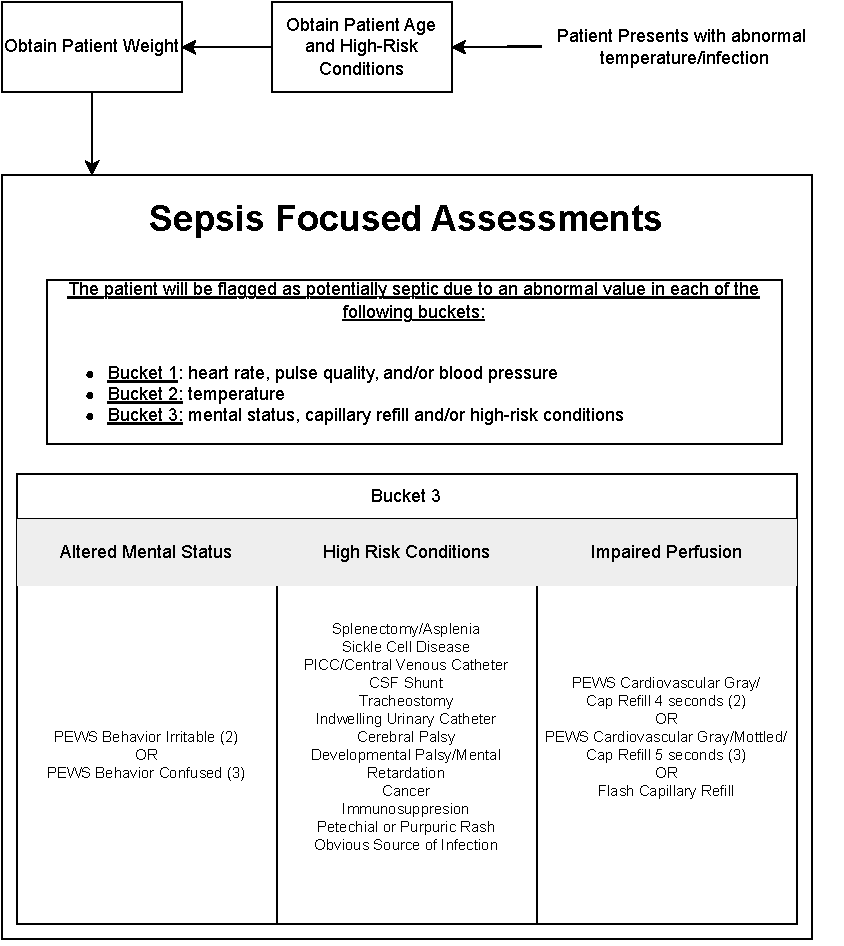
\includegraphics[width=0.43\textwidth]{sepsis-screening-osf}
  %\includegraphics[width=0.5\textwidth]{screening-vitals}
  \caption{Pediatric sepsis screening \BPG{}}\label{fig:sepsis-screening}
\end{figure}

To illustrate characteristics of \BPGs{}, we briefly go over a \BPG{}
for managing sepsis in pediatric cases used at OSF St. Francis Medical Center
in Peoria, Illinois -- a major pediatric hospital in the United States. Note
that for brevity, we refer to said hospital simply as OSF in the remainder of
this section.
Sepsis is life-threatening condition caused by the body's extreme response to
an infection \cite{RhodesICM17}, and is
a major cause of morbidity and mortality in children \cite{Eisenberg2021JP}.
Adverse outcomes can, however, be mitigated through timely
identification and prompt treatment with antibiotics and
intravenous (IV) fluids \cite{Weiss2014CCM,Evans2018JAMA}.
\BPGs{} for screening and management of sepsis in pediatric Emergency
Departments (EDs) have shown effectiveness in screening and management of sepsis \cite{Eisenberg2021JP},
leading to their adoption in many pediatric EDs \cite{Balamuth2017EM,Sepanski2014FP}.

In \figurename{} \ref{fig:sepsis-screening}, we present a simplified version of
the screening section of OSF's sepsis mangement guideline.
In essence, when a patient arrives at the
\ED{} with a fever or an infection, the \HCP{} is supposed to obtain
\begin{enumerate*}[label=(\alph*)]
  \item the patient's age,
  \item any conditions, such as cancer, immunosuppresssion, etc,
    that increase likelihood of sepsis, and
  \item the patient's vital signs, such as heart rate, systolic blood
    pressure, respiratory rate, etc.
\end{enumerate*}
\begin{footnotesize}
  \begin{table}
    \centering
    \begin{tabular}{ | c || c | c | c | }
      \hline
      \textbf{Age}            & \textbf{Heart Rate}   & \textbf{Systolic BP} & \textbf{Temp}  \\
      \hline
      $0d - 1m$               & $>205$                & $<60$                & $<36 \text{ or } >38$ \\
      \hline
      $\geq 1m - 3m$          & $>205$                & $<70$                & $<36 \text{ or } >38$ \\
      \hline
      $\geq 3m - 1y$          & $>190$                & $<70$                & $<36 \text{ or } >38.5$ \\
      \hline
      $\dots$                 & $\dots$               & $\dots$              & $\dots$ \\
      \hline
      $\geq 13y$              & $>100$                & $<90$                & $<36 \text{ or } >38.5$ \\
      \hline
    \end{tabular}
    \caption{Vital Signs Chart}\label{table:vital-signs}
  \end{table}
\end{footnotesize}

This information is then used to check for abnormalities
in clusters of linked information, called \say{buckets}. For instance, if
the patient's heart rate is abnormal, then \say{bucket 1} is said to
have an abnormal value.
Checking for such abnormalities often involves the use of tables, such as
\tablename{} \ref{table:vital-signs} that contains normal ranges indexed by
\emph{age}.
%\footnote{For brevity, we omit some age ranges and vital signs from table
%\ref{table:vital-signs}}.
If the patient has at least one abnormal value in every \say{bucket},
then he/she is flagged as potentially septic.

The \BPG{}-recommended treatment for
sepsis involves multiple concurrent workflows, such as
screening for septic shock, fluid resuscitation, and administering antibiotics.
In \figurename{} \ref{fig:fluid-therapy}, we provide
a version of the fluid resuscitation guideline used
at OSF. Briefly, if the patient is flagged as potentially septic, the guideline suggests
\begin{enumerate*}[label=(\roman*)]
  \item obtaining any fluid-overload risks,
  \item administering normal saline (typically over a period of 15 minutes),
    where the dosage is dictated by risks determined in previous step,
  \item assessing signs of fluid-overload,
  \item evaluating patient responsiveness to normal saline upon completion of
    the administering process, and,
  \item determining whether another fluid bolus should be administered based on
    information from previous steps.
\end{enumerate*}
\begin{figure}[b]
  \centering
  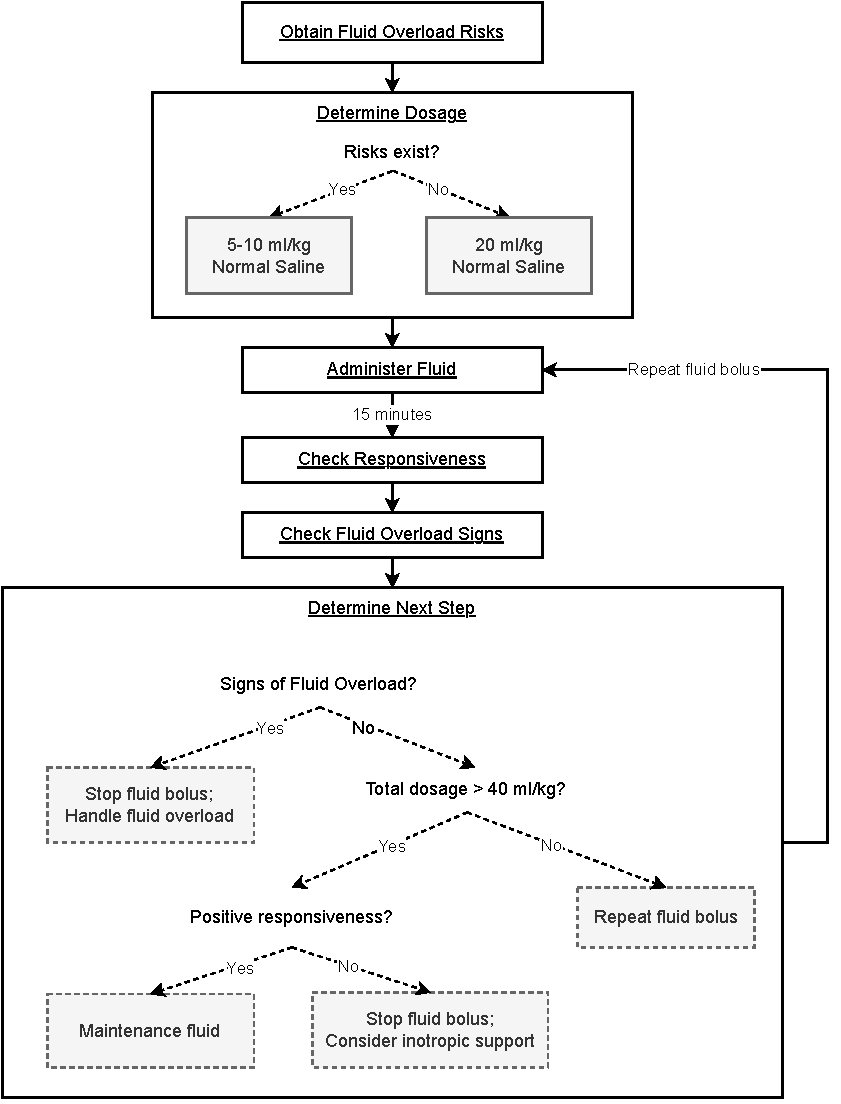
\includegraphics[scale=0.45]{FluidWorkflow-fmcad.pdf}
  \caption{Fluid Resuscitation Guideline}\label{fig:fluid-therapy}
\end{figure}

This real-world \BPG{} exhibits characteristics common
across many \BPGs{}. Specifically \BPGs{} typically:
\begin{itemize}
  \item Involve \stress{concurrent} workflows, such as administering drugs,
    monitoring vitals, performing treatment, etc. There may also be
    inter-workflow interactions. For instance, a diagnosis of sepsis during the
    screening may require modifications to an ongoing course antibitiotics.
  \item Often specified in a \stress{flowchart-like}
    notation. See \cite{AHAFlowcharts} and \cite{CancerCareFlowcharts} for other flowchart-based \BPGs{} for management of \emph{cardiac arrest}, and
    screening, risk-reduction, treatment and survivorship in
    cancer care respectively.
  \item Require communication between \stress{heterogeneous agents} such as
     monitors and Electronic Health Records (EHRs).
  \item Often use \stress{tables} indexed by parameters such as age, weight,
    etc to present normal/abnormal ranges for measurements, or recommended dosages for drugs.
\end{itemize}

Note that the aforementioned characteristics are \emph{not} specific
to one guideline. According to a review paper on \CIGs{} \cite{ClerqAIM03},
such \DSLs{} should additionally
\begin{enumerate*}[label=(\alph*)]
  \item be formally defined, i.e, have a formal syntax and semantics, and
  \item have an execution engine to provide decision support.
\end{enumerate*}


\section{Clinical Decision Support Systems}\label{sec:cdss-background}






\chapter{Hurdles to \CDSS{} Adoption}\label{chapter:hurdles-cdss-adoption}

There is now increasing evidence to suggest that
well implemented \CDSSs{} can significantly improve quality of care
\cite{GargJAMA05,WellsEJPC08}. However, despite several advantages,
several challenges continue to inhibit wider \CDSS{} adoption \cite{Nam17}.
Some challenges are non-technical, i.e., require changes to legislation,
incentive mechanisms and practitioner education and training, and are beyond the
scope of this work. But, several limitations in existing \CDSS{} technology have also
inhibited further adoption. This chapter discusses said challenges, and
the progress made by existing state of art towards addressing them.

Recall, from section \ref{sec:hurdles-cdss-adoption}, that in 2017,
the National Academy of Medicine published a report on \CDSSs{} that
laid out a roadmap to optmize \CDSS{} uptake in medicine. According to the
report, several challenges need to be tackled for wider adoption, such as:


\begin{enumerate}[label=C\arabic*.]
\itemsep0.0em
\item Absence of systematic ways of \emph{validating content}
in a \emph{reliable}, \emph{accessible} and \emph{updateable} manner.
\item Lack of \emph{reliable}, \emph{shareable} \CDSS{} content
that can be easily adopted across healthcare organizations and their (Information
Technology) \IT{} systems.
\item Technical difficulties of sharing due to \emph{need for
  adaptation} to diverse Electronic Health Records (\EHR) systems.
\item \emph{Suboptimal} User Interfaces (\UIs), implementation choices and
workflows.
\end{enumerate}

\section{Addressing Adoption Hurdles}

\CDSS{} first appeared in the 1960s, and have evolved over time
to address aforementioned challenges. The following sections
describe progress made towards addressing aforementioned challnges.

\subsection{Monolithic \CDSSs{}}\label{sec:monolithic-cdss}

Early \CDSSs{} were developed as monolithic standalone systems
that were self-contained, requiring direct user input for clinical data
\cite{RodriguezBook16}. Such systems co-existed with
primitive electronic health records (\EHR{}) systems,
and thus had to rely on manual data entry before administering support.

Several successful \CDSSs{} implementations utilized a standalone
architecture. Early \CDSS{} implementations
such as MYCIN \cite{ShortliffeBook12} required the \HCP{}
to answer a set of questions to provide advice regarding microbial therapy.
Other early \CDSSs{} such as DXplain \cite{BarnettJAMA87} utilized a wide
range of findings (history, data, etc.) to come up with a diagnosis, and
is still in active development.

The reliance on manual entry made using such systems time-consuming. As support for \EHR{} matured,
\CDSSs{} implementations became better integrated with \EHR{} systems
for automated clinical data retrieval.
However, with monolithic systems, the integration was usually \EHR{}-specific \cite{RodriguezBook16}.
Migrating or sharing \CDSS{} content across medical establishments
presented significant challenges as a system designed
for an establishment's \EHR{} system couldn't be used with a different
establishment's \EHR{} system \cite{KawamotoJBI10}.

\subsection{Modular \CDSS{} Architectures}\label{sec:modular-architectures}

In section \ref{sec:cdss-components}, we presented the components that
every guidelines-based clinical decision support can conceptually be decomposed
into. Early \CDSSs{} from section \ref{sec:monolithic-cdss}
were not designed with modularity that enabled sharing components
between different implementations. As the need for scaling \CDSSs{}
across institutions grew, component-based architectures that
enabled \EHR{} agnostic systems to be developed became prevalent \cite{KawamotoJBI10}.

\EHR{}-agnostic architectures represent a significant step towards
addressing several challenges. Such architectures
address C3 as the knowledge-base can be shared across institutions with
different \EHR{} systems. C2 is partially addressed as the
knowledge-base can be independently developed, maintained and distributed.
C4 is also partially addressed as decoupled components, such as the \UI{},
are easier to adapt to \HCP{} preferences.

Over the years, several \CDSS{} implementations have utilized a
components-based architecture. For instance, in \cite{KawamotoJBI10}, the
authors utilize the service-oriented architecture \cite{ErlBook05} to build
a \CDSS{} web service that can be utilized in a completely \EHR{}-agnostic way.
Recent efforts include \CDSSs{} platforms such as
EvidencePoint that enable \CDSS{} to be integrated
closely with the hospital's \EHR{} without being tightly coupled \cite{SolomonJMIR23}.
\EHR{}-agnostic architectures allow decision support to be administered using the
\EHR{}'s \UI{}. Given their prevalence in modern medical establishments,
\EHR{} systems have become integrated into workflows,
and HCPs are accustomed to using them. Dispensing clinical decision
support through the \EHR{}'s \UI{} is vital for adoption, as better workflow
integration can lead to higher adoption \cite{PressJMIR16,LiJMI16}.

Approaches that utilize a component-based architecture
enable medical knowledge to be shared more efficiently.
But, it's possible for medical knowledge itself to be incorrectly
encoded. \BPGs{} are generally expressed as long textual documents meant to
be understood by \HCPs{} \cite{SchiffmanYMI13}. To build a \CDSS{}, the \BPG{} has to be
systematically expressed in a computable medium. This translation process,
referred to as knowledge formalization, is generally ad-hoc, and can be
the source of inconsistencies in encoded medical knowledge
resulting in \CDSSs{} that render wrong advice \cite{ShaharIOS04}.

Typically, in order to translate textual guidelines to a computable
medium, experts in medicine collaborate with computer scientists and
software developers to come up with a requirements document.
This is subsequently utilized to develop the knowledge base, i.e.,
the computer interpretable encoding of the \BPG{} \cite{PelegJBI13} in a
traditional programming language. Thus, the \BPG{} as a
functional specification for the knowledge base.
For instance, in the case of the aforementioned EvidencePoint,
the knowledge base is expressed in  Javascript \cite{SolomonJMIR23}.

However, since computer scientists/software
developers don't understand medicine, and experts in medicine typically
don't understand programming languages,
it's possible for the functional specification, i.e., the \BPG{}, to
diverge from its implementation, i.e., the knowledge base. Thus,
C1 from section \ref{chapter:hurdles-cdss-adoption} remains unaddressed.

\subsection{Computer-Interpretable \BPGs{}}\label{sec:computer-interpetable-bpg}

\CDSSs{} are safety-critical systems, where bugs can have serious consequences.
Thus, ensuring correctness of \CDSSs{} is vital to widespread adoption.
To ensure bugs arising out of divergences between the textual \BPG{}
and its computable translation, i.e., the knowledge base, the gap between
the \BPG{} and the knowledge base must be eliminated. To this end, instead of
encoding \BPGs{} in a conventional programming language, domain-specific
languages (\DSLs{}) for directly expressing \BPGs{} in a computer-interpretable manner can
be utilized. By emphasizing comprehensibility to \HCPs{}, these \DSLs{} enable
\HCPs{} to validate the accuracy of encoded medical knowledge.
A computer-interpretable \BPGs{} can both as the specification, i.e. the textual \BPG{},
and the implementation, i.e., the knowledge base, thereby eliminating the
specification-implementation gap.

In 1989, the Arden Syntax was developed as a result of incompatibility
of medical knowledge between medical institutions \cite{HripcsakCBM94}.
While it was designed to represent simple guidelines,
such as those related to reminders, more complex treatment protocols couldn't
be represented. Arden syntax had a formal Backus-Naur Form (\BNF{})
syntax definition, but no formal semantics, or a standardized execution engine.
Instead, ad-hoc execution engines for the language have been developed over
time \cite{ClerqAIM03}.

Shortcomings regarding ability of the Arden Syntax to represent complex
treatment protocols were addressed by formalisms such as GLIF \cite{PelegAMIA00}
that permit encoding complex guidelines through the use of a multi-layer
approach to represent both high-level medical knowledge and low-level
implementation details. However, just like the Arden Syntax, GLIF lacks
a formal semantics or formal analysis tools.

The need for formal analysis is identified by Asbru: a formalism with formally
defined syntax and semantics \cite{ShaharAMIA96}. In Asbru, a guideline is modeled as a plan
that contains:
\begin{enumerate*}[label=(\roman*)]
  \item intentions that define aims,
  \item conditions that specify when the plan is applicable,
  \item effects that define expected behavior during execution, and,
  \item a body containing other subplans.
\end{enumerate*}
Apart from an execution engine, the Asbru ecosystem also contains
other tools, such as a model checker for verification \cite{BaumlerSPIN06}.
However, the formal semantics of Asbru have been only partially defined, and
is insufficient to implement tools for the language \cite{SuttonAMIA03}.
The importance of a complete formal-semantics is identified and addressed
by PROforma \cite{SuttonAMIA03}, another formalism that uses plans to
model guidelines. A PROforma plan is made of a sequence of tasks.
The plan defines constraints on their enactment, and circumstances
for termination (for example, exceptions) \cite{SuttonAMIA03}. But, despite
having complete formal semantics, PROforma's semantics is not executable.
Therefore, an interpreter and analysis tools have to be implemented in an
ad-hoc manner.

Over the years, significant progress has been made towards making \CDSSs{}
safer, easier, effective and cheaper. In section \ref{sec:monolithic-cdss},
the earliest \CDSSs{} attempted to increased adherence to evidence-based best practices
at medical establishments. To ensure \CDSSs{} could be scaled better,
components-based architectures, discussed in section
\ref{sec:modular-architectures} enabled medical knowledge to
be developed and maintained independently of other components (such as system
\UI{}). To ensure that medical knowledge is indeed encoded correctly,
several \DSLs{} that eliminate the gap between a textual \BPG{} and
the \CDSS{}' knowledge base have been developed. However,
the following issues still remain:
\begin{itemize}
  \item Interpreters and compilers for said \DSLs{} are developed in an
    ad-hoc way, and can be prone to bugs that manifest during execution.
  \item There is a lack of formal analysis tools such as model checkers and
    program verifiers that can be utilized to establish that the
    computer-interpretable \BPGs{} satisfy desired safety and liveness
    properties.
  \item \DSLs{} lack complete formal semantics that can be utilized
    as a language model for a suite of formal analysis and execution tools.
\end{itemize}

Addressing aforementioned issues is vital to improving \CDSS{} adoption.
In order to have trustworthy and useable computer interpretable \BPGs{},
it's important to buttress  \HCP{}-friendly \DSLs{}
with a suite of formal analysis tools that can establish desired safety
properties, thus comprehensively addressing C1.


\chapter{Related Work}

In chapter \ref{chapter:hurdles-cdss-adoption}, we provided a brief
overview of existing approaches and their limitations. This chapter
provides a comprehensive discussion of related approaches. Recall
from section \ref{sec:modular-architectures} that implementing a guidelines-based
clinical decision support system requires collaboration between
experts in medicine and software engineers for knowledge formalization, i.e.,
the process of encoding medical knowledge in textual
\BPGs{} in some programming language. Using a conventional programming
language for knowledge formalization can lead to an inaccurate
encoding medical knowledge, as experts in medicine, being unaccustomed
to computer programming, cannot validate the accuracy of the encoding.
To address this, \DSLs{} designed specifically for expressing
\BPGs{} in a computer-interpretable format are utilized. \BPGs{} expressed
in such languages can serve as both textual guideline documents and knowledge
bases in \CDSSs{}. But, medical knowledge in \BPGs{} has also been expressed
and formalized using other non domain-specific approaches. The discussion in
this chapter has also been split along the same lines. In section
\ref{sec:dsl-based-approaches}, we discuss approaches involving \DSLs{} for
computer interpretable guidelines. In \ref{sec:general-approaches}, we
discuss other approaches that aren't specific to \BPGs{}.

\section{\DSL{}-based Approaches}\label{sec:dsl-based-approaches}

\subsection{Arden Syntax}

The Arden Syntax is among the earliest and most widely-used
standards for expressing medical logic, with the first
draft of the standard appearing in 1989.
It was also among the earliest attempts to create a domain
specific langauge specifically for use in \CDSSs{} \cite{SamwaldJBI12}.

In Arden Syntax, code is organized into self-contained medical
logic modules (\MLMs{}) that have a well-defined structure to
separate higher-level medical logic from low-level implementation
details such as variable declarations. The language continues to
evolve to accomodate diverse uses, and is supported by multiple execution
engines \cite{AnandMed04}.

\section{General Approaches}\label{sec:general-approaches}







\chapter{Semantics-First Approach to Clinical Decision Support}

In \autoref{chapter:introduction}, we explained that, despite
advances in medicine, mortality and costs associated with preventable
medical errors (\PMEs{}) remain unacceptably high. In
\autoref{chapter:background}, we explained how systems that
assist healthcare practitioners (\HCPs{}) with situation-specific
advice based on evidence-based best practice guidelines (\BPGs{}),
called clinical decision (\CDSSs{}) can reduce both mortality
and costs associated with \PMEs{}. But, despite their potential,
the uptake of such systems in practice is hindered by challenges
that were introduced in \autoref{sec:hurdles-cdss-adoption}, and
discussed in depth in \autoref{chapter:hurdles-cdss-adoption}.
In brief, the following challenges (Cs) were outlined:
\begin{enumerate}[label=C\arabic*.]
\itemsep0.0em
\item Absence of systematic ways of \emph{validating content}
in a \emph{reliable}, \emph{accessible} and \emph{updateable} manner.
\item Lack of \emph{reliable}, \emph{shareable} \CDSS{} content
that can be easily adopted across healthcare organizations and their (Information
Technology) \IT{} systems.
\item Technical difficulties of sharing due to \emph{need for
  adaptation} to diverse Electronic Health Records (\EHR) systems.
\item \emph{Suboptimal} User Interfaces (\UIs), implementation choices and
workflows.
\end{enumerate}

\begin{figure}[th!]
  \centering
  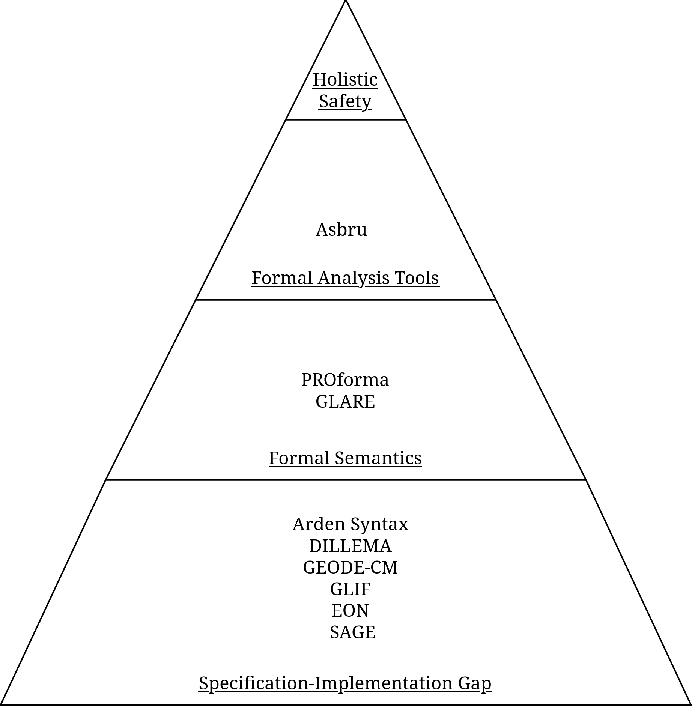
\includegraphics[width=0.5\textwidth]{pyramid}
  \caption{Existing \DSLs{} for Computer Interpretable Guidelines}\label{fig:existing-work-pyramid}
\end{figure}

Over the years, significant progress has been made towards
addressing these challenges. In \autoref{chapter:related-work},
we discussed how existing approaches have attempted to
address said challenges, and their limitations. Specifically,
in \autoref{sec:related-work-discussion}, we outlined major
themes that these approaches adopt to tackle these challenges.
This is further illustrated by the pyramid diagram in \autoref{fig:existing-work-pyramid}, where aforementioned themes are
underlined in the pyramid's various rungs.
As is typical, approaches that appear in higher rungs also
have characteristics of ones below them. For example, while guidelines expressed in
the Arden Syntax eliminate the specification-implementation gap by being
both \HCP{}-comprehensible and interpretable, they cannot be formally analyzed
due to lack of analysis tools in the ecosystem. Asbru-based guidelines
on the other hand not only eliminate the specification-implementation gap, but can also be
formally analyzed using support for KIV-based verification in the Asbru
ecosystem (see \autoref{sec:kiv-verification}).

As is evident in \autoref{fig:existing-work-pyramid}, no
existing approach covers the \say{holistic safety} rung of the pyramid.
Recall from \autoref{sec:related-work-discussion} that we say an
approach tackles \say{holistic safety} if,
besides support for analyzing guidelines,
analysis and execution tools also have correctness guarantees.
In this work, we argue that such guarantees are necessary for
trustworthy \CDSSs{}. We attempt to address \say{holistic safety}
systematically by developing a \emph{semantics-first approach} for
building clinical decision support systems. In this context, by semantics-first
we mean that:
\begin{itemize}
  \item The semantics of the programming language for defining said knowledge is
    formally defined, from which execution and analysis tools are derived in a
    correct by construction manner, leading to holistic safety.
  \item The semantics of medical knowledge are expressed accurately.
\end{itemize}
At the core of our approach is a novel domain-specific language for expressing
medical knowledge called $\MediK{}$ (pronounced Medi-Kay). By being comprehensible to domain experts
in medicine, $\MediK{}$-based computer interpretable guidelines can serve
both as a guideline's non-executable \HCP{}-comprehensible description, i.e.,
the specification, and its encoding in a computable medium, i.e., the
implementation, thereby eliminating any specification-implementation gap.

The remainder of this chapter is structured as follows:
\autoref{sec:semantics-first} briefly describes the semantics-first philosophy.
Next, \autoref{sec:k-framework} describes $\K$ -- the language semantic
framework that $\MediK{}$'s are expressed in. Finally,
\autoref{sec:semantics-first-pitfalls} describes potential pitfalls
of following the semantics-first philosophy.

\section{Semantics-First Approach}\label{sec:semantics-first}

The semantics-first approach prescribes a systematic way of
developing programming languages. Instead of implementing
tools for a language, such as interpreters, compilers and
model checkers in ad-hoc manner, the approach states that the
first step in developing said tools must be to formally define
the language's semantics. As show in \autoref{fig:semantics-first},
once defined, all tools for the language
can then be automatically derived from the semantics. Moreover, since
the tools utilize the semantics, they are, by definition,
correct-by-construction.

While following the semantics-first philosophy might seem like an obvious choice
in language design, its adoption in practice is far from ideal.
Conventional practice in the programming language and formal
methods community is still to develop analysis and execution tools for each
programming language from scratch \cite{ChenSETSS19}, as illustrated
in \autoref{fig:conventional-pl-development} from
\cite{ChenSETSS19}. But, this approach has several
disadvantages:
\begin{itemize}
  \item Implementing tools that perform the same function for
    different languages incurs unnecessary development and maintenance cost.
    As shown in \autoref{fig:conventional-pl-development}, if there are
    $l$ languages, where each has $t$ tools, then a total of $l \times t$
    tools have to be developed and maintained over time.
  \item Tools are often based on informal descriptions of language semantics,
    leaving developers to extrapolate finer details of the language's semantics,
    leading to inconsistencies.
    For instance, in \cite{ParkPLDI15}, it was found
    that ECMAScript 5.1-compliant JavaScript engines
    in mainstream web browsers behaved differently from each other
    for certain complex JavaScript programs.
  \item As newer versions of a language are introduced, each
    tool for the language has to be updated to ensure support for the latest
    version. This again results in duplicated work.
\end{itemize}
\begin{figure}[t!]
  \centering
  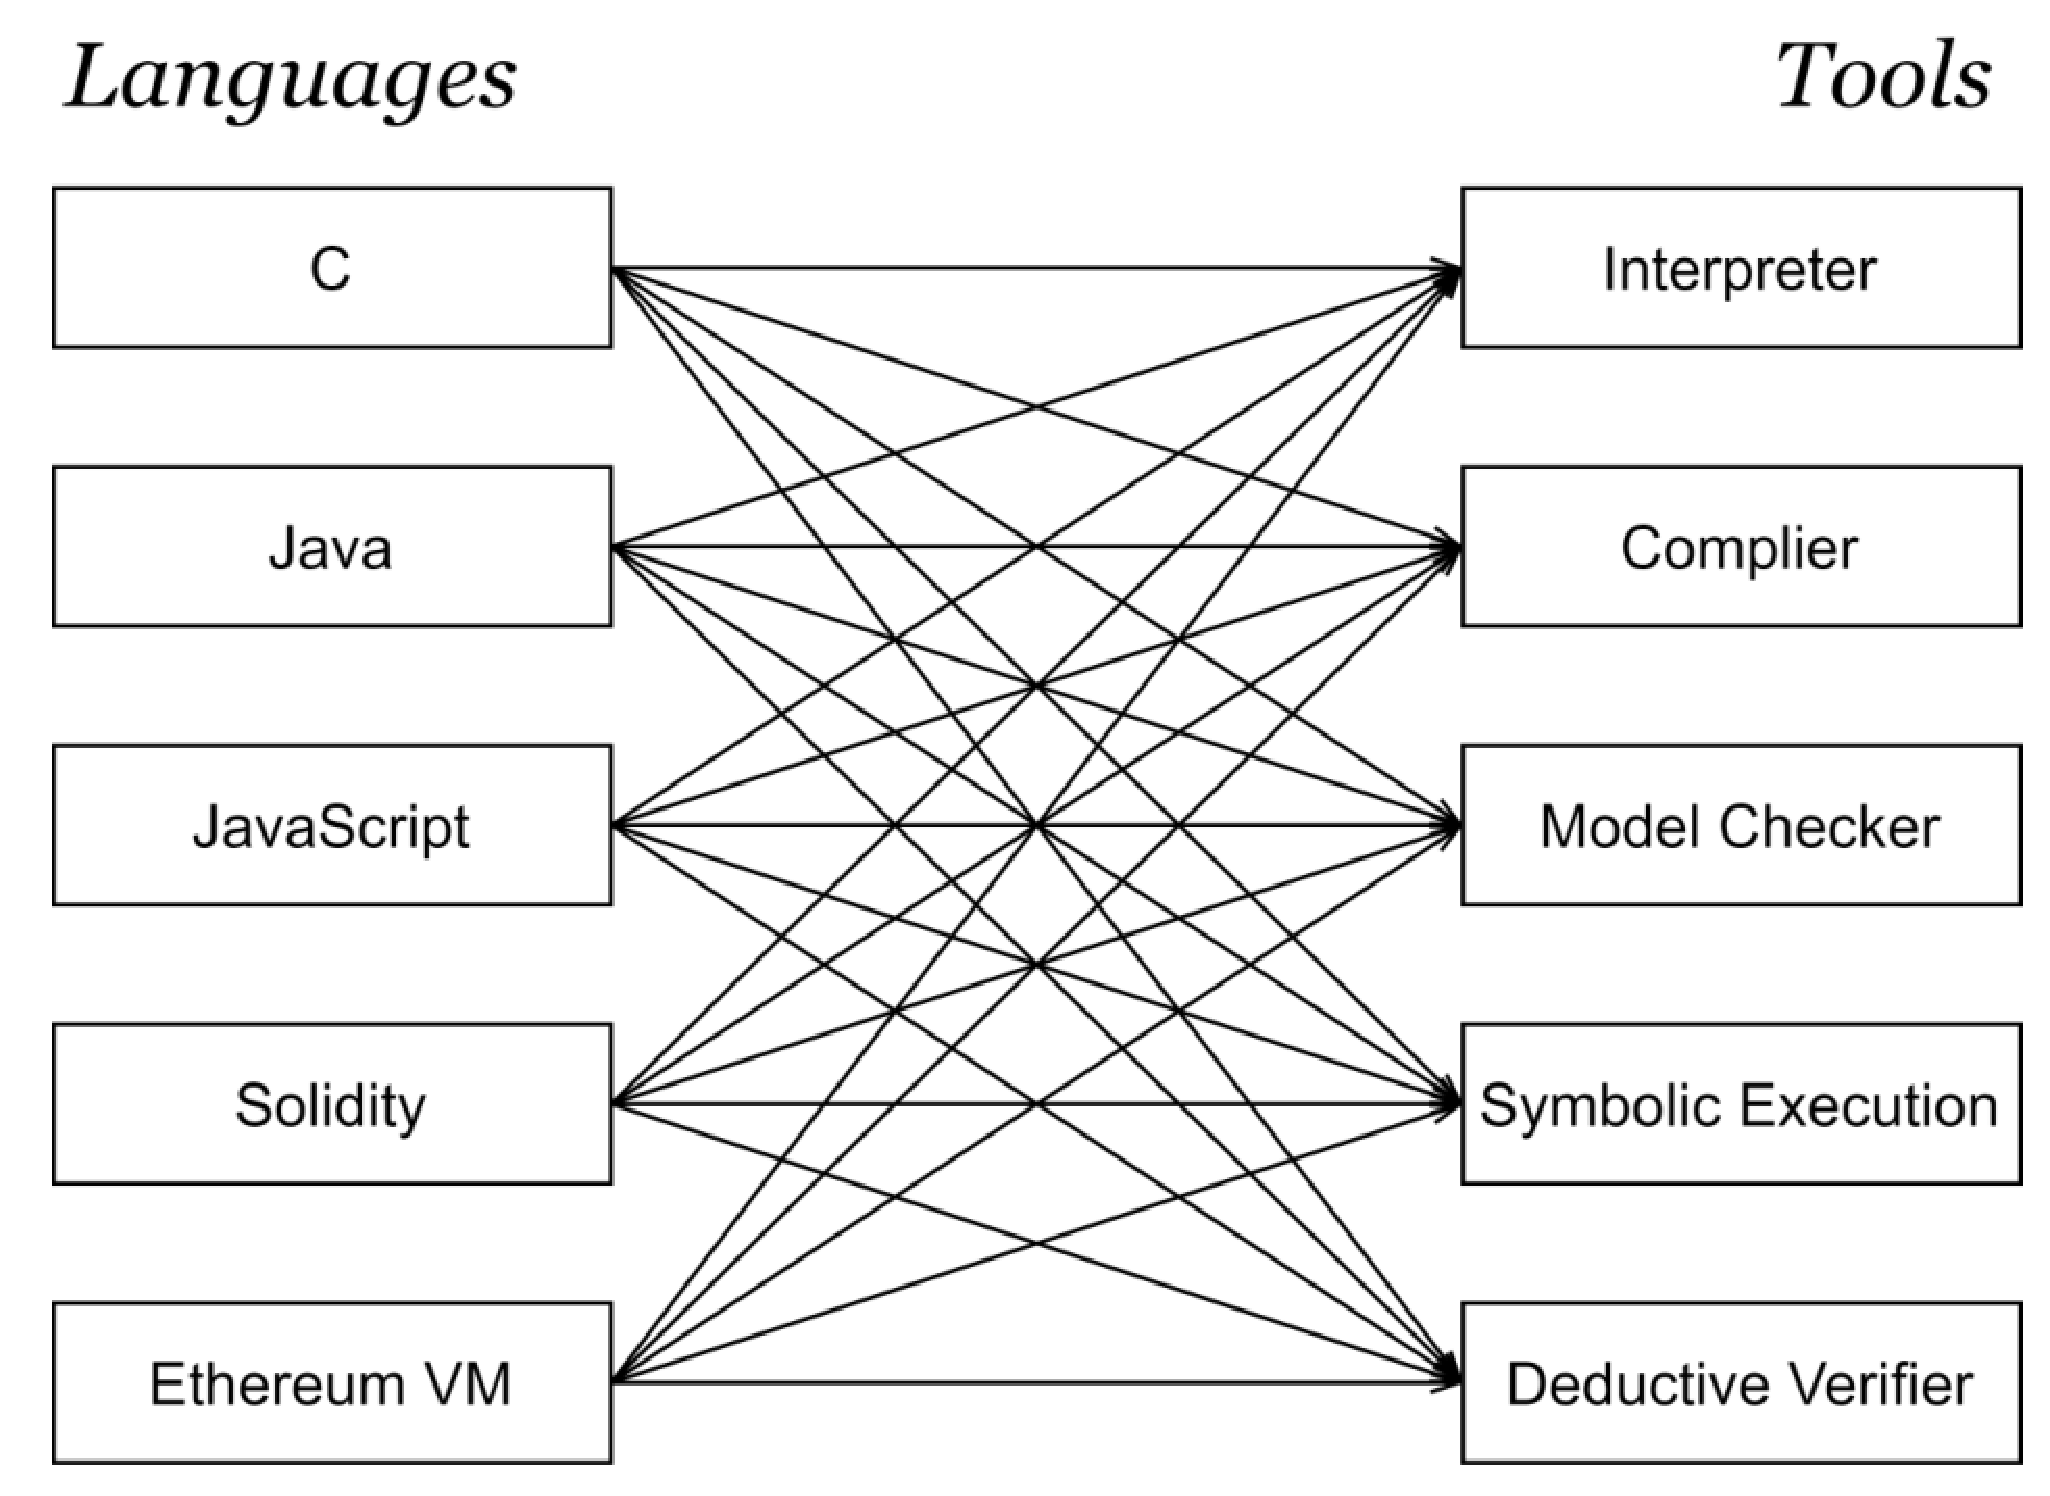
\includegraphics[width=0.6\textwidth]{conventional-pl-development}
  \caption{State-of-Art in Programming Language Design}\label{fig:conventional-pl-development}
\end{figure}

\subsection{Why build \CDSSs{} using Semantics-First?}

In section \ref{sec:semantics-first}, we described benefits
of using the semantics-first approach for developing regular programming
language. But, these differences become starker when semantics-first
is compared against the conventional approach shown in \autoref{fig:conventional-pl-development} in context of domain-specific language for
expressing medical guidelines. Specifically, as such a language will be utilized
in safety-critical settings, it is vital that the language:
\begin{itemize}
  \item Has an \emph{unambiguous}, \emph{formal}
    semantics that can serve as a reference for developing tool support for it.
    This is necessary to ensure that
    tools are free of behavioral inconsistencies due to ambiguities in the
    semantics.
  \item Is supported by a rich formal analysis tools that can
    be used to analyze programs.
    Implementing such tools from scratch would require significant effort.
  \item Can evolve quick to incorporate
    \begin{enumerate*}[label=(\roman*)]
      \item lessons from expressing medical guidelines in it, and,
      \item \HCP{} feedback, specifically regarding comprehensibility.
    \end{enumerate*}
    This can be challenging when using the approach shown in \autoref{fig:conventional-pl-development}, as
    every change to the language's semantics would require corresponding
    changes to all relevant tools, and additional effort to maintain
    different versions, making the development process extremely tedious.
\end{itemize}

\section{The $\K{}$ Framework}\label{sec:k-framework}

In this section, we introduce $\K{}$: a rewrite-based executable semantics
in which programming languages can be defined through configurations and rules
\cite{KframeworkUrl}. Once the semantics of a programming language has been
defined, $\K{}$ automatically generates all tools depicted in \autoref{fig:semantics-first}, such as an interpreter, compiler,
model-checker and deductive verifier for the language. $\K{}$ has been successfully
utilized to formalize semantics of large real-world languages, such as
C \cite{HathhornPLDI15}, Java \cite{BogdanasPOPL15} and
Javascript \cite{ParkPLDI15}, and analyze non-trivial programs
\cite{StefanescuOOPSLA16,ParkFSE18}.

The remainder of this section introduces relevant features of
$\K{}$ by describing the $\K{}$ semantics of an example language called
Imp. This introduction to $\K{}$ provides necessary background
for upcoming chapters that discuss the $\MediK{}$ \DSL{} through the
use of $\K{}$ notation and concepts.

\subsection{Defining Languages in $\K$}\label{sec:semantics-in-k}

A typical $\K$ definition of a language consists of the following components:
\begin{itemize}
  \item Syntax: Defined in \BNF{}-like notation, and utilized by $\K$
    to generate a parser for the language.
  \item Configuration: Organizes the program execution state
    into units called \emph{cells} that may be nested.
  \item Rules: Operate over configuration segments and define program
    evolution via rewrites.
\end{itemize}
We now discuss aforementioned components in the context of the Imp
language. Imp is a simple imperative programming language
inspired by C and Java that supports arithmetic and boolean expressions and
statements such as variable declaration and assignment, branching (\inlineimp{if})
and looping (\inlineimp{while}).

\autoref{lst:imp-syntax} and \autoref{lst:imp-semantics},
define syntax and semantics of Imp respectively.
$\K{}$ code must be place inside an organizational unit called a
\inlinek{module} that has a name, and can import other \inlinek{module}(s).
For example, \inlinek{module IMP-SYNTAX ... endmodule}
between \autoref{lstline:imp-module-start} and
\autoref{lstline:imp-module-end} of \autoref{lst:imp-syntax} defines
a $\K{}$ \inlinek{module} named \inlinek{IMP-SYNTAX} containing Imp's
grammar. $\K{}$ provides builtin support for domains such as natural
numbers, integers, booleans and program identifiers
under a \inlinek{module} named \inlinek{DOMAINS}.
\autoref{lstline:imp-syntax-import} \inlinek{imports}
the syntax definition of $\K{}$'s \inlinek{DOMAINS} module
to enable parsing integers and booleans in Imp programs.

\begin{lstlisting}[float=ht,
  frame=single,
  style=ksty,
  language=k,
  numbers=left,
  numbersep=5pt,
  caption={Imp Syntax in $\K$},
  label={lst:imp-syntax}
]
module IMP-SYNTAX                                               @\label{lstline:imp-module-start}@
  imports DOMAINS-SYNTAX                                        @\label{lstline:imp-syntax-import}@
  syntax AExp  ::= Int | Id                                     @\label{lstline:imp-aexp-start}@
                 | "-" Int
                 | AExp "/" AExp              [left, strict]    @\label{lstline:imp-aexp-div}@
                 | "(" AExp ")"               [bracket]
                 > AExp "+" AExp              [left, strict]    @\label{lstline:imp-aexp-end}@
  syntax BExp  ::= Bool
                 | AExp "<=" AExp             [seqstrict]
                 | "!" BExp                   [strict]
                 | "(" BExp ")"               [bracket]
                 > BExp "&&" BExp             [left, strict(1)] @\label{lstline:imp-bexp-and}@
  syntax Block ::= "{" "}"
                 | "{" Stmt "}"
  syntax Stmt  ::= Block                                        @\label{lstline:imp-stmt-block}@
                 | Id "=" AExp ";"            [strict(2)]       @\label{lstline:imp-stmt-assgn}@
                 | "if" "(" BExp ")"
                   Block "else" Block         [strict(1)]
                 | "while" "(" BExp ")" Block                   @\label{lstline:imp-stmt-while}@
                 > Stmt Stmt                  [left]            @\label{lstline:imp-stmt-comp}@
  syntax Pgm ::= "int" Ids ";" Stmt                             @\label{lstline:imp-pgm}@
  syntax Ids ::= List{Id,","}                                   @\label{lstline:imp-ids}@
endmodule                                                       @\label{lstline:imp-module-end}@
\end{lstlisting}

\emph{Syntax} in $\K{}$ is defined using BNF-like notation; terminals are enclosed
in quotes, and non-terminals begin with an uppercase. For example,
consider the declaration of Imp arithmetic expressions between
\autoref{lstline:imp-aexp-start} and \autoref{lstline:imp-aexp-end}. On
\autoref{lstline:imp-aexp-start} $\K$'s builtin support
for integers (\inlinek{Int}) and program identifiers
(\inlinek{Id}) is used to support arithmetic expressions over program variables.
Beyond simply defining the syntax, $\K{}$ also allows assigning semantics to
constructs through the use of \emph{attributes} specified as a comma-separated list
inside square brackets (\inlinek{[..]}) placed immediately after the \BNF{} production.
For example, On \autoref{lstline:imp-aexp-div} and \autoref{lstline:imp-aexp-end},
the attribute \inlinek{left} is used to declare the
corresponding operator as left associative. The \inlinek{strict} attribute is used
to assign \emph{evaluation strategies}. Note its use
on \autoref{lstline:imp-aexp-div} and \autoref{lstline:imp-aexp-end}, signifying
that both operand sub-expressions must be completely evaluated before the
before the corresponding operator (\inlinek{/}, \inlinek{+}) is evaluated.
Note that the order in which the arguments are evaluated is non-deterministic,
and, all operands will be evaluated before the operator is evaluated.
To enforce a particular order, or, to choose a subset of the operands, a
list of operand positions specifying the desired order can be supplied to
\inlinek{strict}. For example, \inlinek{strict(2, 1)} would make $\K$
evaluate the second argument before the first. This is particularly
useful for defining constructs like short-curcuit (\inlineimp{&&}) boolean
expression on \autoref{lstline:imp-bexp-and}, where \inlinek{strict(1)}
ensures that the left operand is evaluated first, allowing the right to only
be evaluated if the left evaluates to \inlinek{true}.
Similarly, for an assignment statement on \autoref{lstline:imp-stmt-assgn}
the \inlinek{strict(2)} indicates that the second argument, i.e., the
expression to the right of the \inlineimp{=} sign must be evaluated before
the identifier on the left of the \inlineimp{=} is updated.

$\K{}$ also allows operator precedence to be specified as a part of the
syntax definition. On \autoref{lstline:imp-aexp-end},
the \inlinek{>} signifies that all preceding productions have higher precedence,
i.e., bind tighter, than the production for addition (\inlinek{+}).
Similarly, \autoref{lstline:imp-stmt-comp} defines statement composition.
Thus, preceding \inlinek{Stmt} productions
(\autoref{lstline:imp-stmt-block}-\autoref{lstline:imp-stmt-while}), that define
blocks (\inlinek{\{..\}}) and standalone statements such as variable assignment and
while loop have higher precedence, indicated by \inlinek{>} on \autoref{lstline:imp-stmt-comp}.

On \autoref{lstline:imp-pgm}, an Imp program is defined to start with a list of program variable
declarations (\inlinek{"int" Ids ";"}) followed by other statements. Note the
definition of a list of identifier (\inlinek{Ids}) on \autoref{lstline:imp-ids}. In $\K{}$,
\inlinek{List\{...\}} is used to define syntactic-lists, where the first
argument is the production of list elements, and the second the list de-limiter.
Thus, \inlinek{List\{Id, ","\}} defines a comma-separated list of program identifiers.

Once the \emph{syntax} has been defined, $\K$ can utilize it to generate a
parser, which can be used to generate abstract
syntax trees (\ASTs{}) for programs. The program's \AST{} forms a part of the larger
program state, over which semantics are defined through rules.
The $\K$ semantics of any language has two components:
\begin{itemize}
  \item A \emph{Configuration} that organizes the state
    into units called \emph{cells}, that may be nested.
  \item \emph{Rules} that operate over \emph{configuration}-segments
    to desribe evolution of state during execution.
\end{itemize}
For Imp, \autoref{lst:imp-semantics} has aforementioned
components inside \inlinek{module IMP}.
Note that the syntax and semantics exist in separate modules,
where the semantics module \inlinek{imports}
the syntax module. This is by convention, and
has the following advantages:
\begin{enumerate}[label=\alph*)]
  \item Rules can operate directly over the language's syntax,
    making them easier to specify and comprehend.
  \item With the syntax and semantics residing in separate modules,
    $\K$ can be instructed to use only the syntax module for parsing programs.
    This allows users to define additional syntactic constructs in the semantics module
    for use in rules. If a combined syntax and semantics module is used instead,
    any constructs defined solely for use in rules
    would unintentionally become part of the language's syntax,
    and be accepted by the parser.
\end{enumerate}

\begin{lstlisting}[float=t,
  frame=single,
  style=ksty,
  language=k,
  numbers=left,
  numbersep=5pt,
  caption={$\K$ Semantics of Imp},
  label={lst:imp-semantics}
]
module IMP
  imports IMP-SYNTAX
  imports DOMAINS
  syntax KResult ::= Int | Bool             @\label{lstline:imp-kresult}@

  configuration <T>                         @\label{lstline:imp-config-start}@
                  <k> $PGM:Pgm </k>         @\label{lstline:imp-pgm-var}@
                  <state> .Map </state>     @\label{lstline:imp-pgm-state}@
                </T>                        @\label{lstline:imp-config-end}@

// AExp
  rule <k> X:Id => I ...</k> <state>... X |-> I ...</state> @\label{lstline:imp-assgn-rule}@
  rule I1 / I2 => I1 /Int I2  requires I2 =/=Int 0
  rule I1 + I2 => I1 +Int I2                @\label{lstline:imp-add-rule}@
  rule - I1 => 0 -Int I1
// BExp
  rule I1 <= I2 => I1 <=Int I2
  rule ! T => notBool T
  rule true && B => B
  rule false && _ => false
// Block
  rule {} => .   [structural]
  rule {S} => S  [structural]
// Stmt
  rule <k> X = I:Int; => . ...</k> <state>... X |-> (_ => I) ...</state>
  rule S1:Stmt S2:Stmt => S1 ~> S2  [structural] @\label{lstline:imp-stmt-decomp}@
  rule if (true)  S else _ => S  @\label{lstline:imp-if-true-rule}@
  rule if (false) _ else S => S  @\label{lstline:imp-if-false-rule}@
  rule while (B) S => if (B) {S while (B) S} else {}  [structural]
// Pgm
  rule <k> int (X,Xs => Xs);_ </k> <state> Rho:Map (.Map => X|->0) </state> @\label{lstline:imp-vardec-rule}@
    requires notBool (X in keys(Rho))  @\label{lstline:imp-vardec-requires}@
  rule int .Ids; S => S  [structural]  @\label{lstline:imp-emptydec-rule}@

endmodule
\end{lstlisting}

\subsubsection{Configurations}\label{sec:k-configuration}

The configuration is defined using the keyword \inlinek{configuration},
followed by an unordered list of \emph{cells},
which may be nested and are specified using an XML-like notation.
For instance, \inlinek{<foo> <bar> ... </bar> </foo>}
corresponds to $\K$ \emph{cells} named
\inlinek{foo} and \inlinek{bar} respectively, where \inlinek{bar}
is nested under \inlinek{foo}.
Imp's configuration is defined
between \autoref{lstline:imp-config-start} and \autoref{lstline:imp-config-end},
and consists of a top-level cell \inlinek{<T>} containing cells
\inlinek{<k>} and \inlinek{<state>} on \autoref{lstline:imp-pgm-var} and
\autoref{lstline:imp-config-end} respectively. In $\K{}$,
the \inlinek{<k>} cell typically contains the \AST{} of the executing
program, indicated by its contents \inlinek{$PGM:Pgm}.
During execution, $\K{}$ will attempt to parse the program being executed
using the production \inlinek{Pgm} defined on \autoref{lstline:imp-pgm} of
\autoref{lst:imp-syntax}. If parsing is successful, $\K{}$ will replace
\inlinek{$PGM} with the parsed \AST{}. The \inlinek{<state>} cell,
as the name suggests, will hold a map of
program identifiers and values they acquire during execution.
Said map is initially empty, denoted by \inlinek{.Map}.
The dot (\inlinek{.}) in $\K{}$ denotes \emph{nothing} or \emph{empty}.
Thus, \inlinek{.Map} denotes an empty map.

\subsubsection{Rules}\label{sec:k-rules}
$\K$ \emph{rules} operate over configuration segments and define evolution of
program state. When specifying a rule $\K{}$, only relevant parts of the
configuration need to be mentioned---$\K{}$ completes the rest of the
configuration through a mechanism called \emph{configuration abstraction}.
This allows rules to be concise,
enhancing readability and making them easier to write. For example,
consider the rule for addition on \autoref{lstline:imp-add-rule}.
Simply put, the rule specifies that if the term at the top of the \inlinek{<k>}
cell is an addition expression, then it should be \emph{rewritten} to
addition in the integer domain \inlinek{+Int}. But, even though the
rule is intended to simplify the top of the \inlinek{<k>} cell,
no cells are explicitly mentioned. This is because:
\begin{itemize}
  \item If no cell is mentioned, $\K$ assumes that rule applies at the top of
    the $\K{}$ cell.
  \item All other parts of the configuration are assumed to remain unchanged.
\end{itemize}

Now we describe rules in greater depth.
A rule begins with the keyword \inlinek{rule}
and is a statement of the form $\varphi \To \psi$, where
$\varphi$, $\psi$ are \emph{patterns} over configuration terms and $\K$ variables.
We say $\varphi$ is the LHS and $\psi$ is the RHS of the rule.
We define a \emph{substitution} $\theta$ to be a map from $\K$-variables to terms.
Given pattern $\varphi$ and \emph{substitution} $\theta$, we say
$\varphi\theta$ is the pattern obtained by replacing every variable $v$ in
$\varphi$ with $\theta(v)$. We say pattern $\varphi$ matches
term $\tau$ iff there exists a substitution $\theta$ s.t. $\tau = \varphi\theta$.
During execution, if the current configuration term
$\tau$ \emph{matches} the LHS $\varphi$ of rule $\varphi \To \psi$
with substitution $\theta$, then $C$ is rewritten to $\psi\theta$.
For example, the addition rule on \autoref{lstline:imp-add-rule}.
$\K$-variables always begin with an uppercase, and may be suffixed with
\inlinek{:S}, where \inlinek{S} is the variable's sort. In the case
of the addition rule, $\K$ can \emph{infer} that the sort of
\inlinek{I1} and \inlinek{I2} is \inlinek{Int}, as operands of the
buitin operator \inlinek{+Int} can only be integers (\inlinek{+Int}
is addition in the domain of integers). Thus, the \LHS{} \inlinek{I1 + I2}
\emph{match} term \inlinek{2 + 3} (of sort \inlinek{AExp})
with substitution
\inlinekmath{$\theta = $(I1\ $\mapsto$ 2, I2\ $\mapsto$\ 3)} and rewrite it \inlinek{2 +Int 3}, i.e. \inlinek{5}, as
\inlinek{+Int} is $\K$-builtin for integer addition.

We now discuss execution of an entire program to introduce $K{}$ nuances
relevant to later chapter. Imp's grammar dictates that an
Imp program (denoted by production \inlinek{Pgm} on
\autoref{lstline:imp-pgm} of \autoref{lst:imp-syntax})
must declare all variables at the start of execution. Consider
the simple program \inlinemedik{int x; x = 2 + 3;}.
At the start of execution, \K{} replaces the \inlinek{$PGM}
in the configuration declaration with the program's \AST{}.
Thus, we get the following initial configuration:
\begin{lstlisting}[language=k,style=ksty,backgroundcolor=\color{white}]
<T>
  <k> int x, .Ids; x = 2 + 3; </k>
  <state> .Map </state>
</T>
\end{lstlisting}
where \inlinek{.Ids} is the identity element for the user-defined
list of program identifiers, and \inlinek{.Map} is the map identity
from the initial configuration declaration on \autoref{lstline:imp-pgm-state}
Now the rule for variable declaration on \autoref{lstline:imp-vardec-rule}
can match with substition \inlinekmath{(X $\ \mapsto\ $ x, Xs\ $ \mapsto\ $ .Ids,
Rho $\ \mapsto\ $.Map)}
to rewrite the configuration to:
\begin{lstlisting}[language=k,style=ksty,backgroundcolor=\color{white}]
<T>
  <k> int .Ids; x = 2 + 3; </k>
  <state> x |-> 0 </state>
</T>
\end{lstlisting}
Note the following conveniences that \K{} offers to make writing rules easier:
\begin{enumerate}[label=\roman*)]
  \item The use of parenthesis limi scope of the rewrite to the
    list of program identifiers. Localized rewriting reduces redundancy
    as only relevant parts of a term have to be mentioned on the \RHS{} of the
    rule.
  \item The underscore \inlinek{_} following \inlinek{int (X, Xs => Xs);}
    on \autoref{lstline:imp-vardec-rule}
    is an \emph{anonymous} variable that matches the remainder to the program.
    Since it's not anywhere on the \RHS{}, there is no need to provide an
    explicit variable name.
\end{enumerate}
Also that the rule has a side condition, expressed through the keyword \inlinek{requires}
on \autoref{lstline:imp-vardec-requires}. This forces the rule to only apply if
the program identifier has not already been declared. For instance,
a program that starts with \inlineimp{int x, x;} will not execute to completion.
Next, the rule on \autoref{lstline:imp-emptydec-rule} will eliminate
\inlinek{int .Ids;}, leaving the following configuration after the rewrite:
\begin{lstlisting}[language=k,style=ksty,backgroundcolor=\color{white}]
<T>
  <k> x = 2 + 3; </k>
  <state> x |-> 0 </state>
</T>
\end{lstlisting}
Also note that the rule does not explicitly mention the cell on which
it is intended to operate. In $\K$, a rule that doesn't
mention any cells is implicitly assumed to apply on top of the
\inlinek{<k>} cell. As the \inlinek{<k>} cell typically
contains the program being executed, not having to explicitly
mention the cell allows the rule to only show how constructs in the language
affect execution. For instance, the rules on \autoref{lstline:imp-if-true-rule}
and \autoref{lstline:imp-if-false-rule} depict that for an
\inlineimp{if(condition) \{...\}} statement,
if the \inlineimp{condition} is true, the \inlineimp{if} block is taken,
else whatever comes after is taken.

Next, consider the assignment rule on \autoref{lstline:imp-assgn-rule} of
\autoref{lst:imp-semantics}. The rule uses two variables: \inlinek{X} and \inlinek{I}
with sorts \inlinek{Id} and \inlinek{Int} respectively. Since the \inlinek{<k>}
cell in our running example has \inlinek{x = 2 + 3;}, we expect the assignment
rule to apply at some point and update the \inlinek{<state>} accordingly.
But, the rule cannot apply as the \RHS{} of the assignment, i.e., the expression
\inlinek{2 + 3}, is not of sort \inlinek{Int}, which needs to be evaluated
first. This in \K{} is enabled by evaluation strategies.
Recall that the attribute assignment statement has the attribute
\inlinek{strict(2)} (\autoref{lstline:imp-stmt-assgn} of
\autoref{lst:imp-syntax}), denoting that the second argument of the
construct must be evaluated first. Thus,
$\K$ will \emph{heat}, or pull-out the second
argument for evaluation. This results in the configuration:
\begin{lstlisting}[language=k,style=ksty,backgroundcolor=\color{white}]
<T>
  <k> 2 + 3 ~> x = []; </k>
  <state> x |-> 0 </state>
</T>
\end{lstlisting}
In $\K{}$, \lstinline[style=inlineksty]{~>} means \emph{followed-by}, i.e.,
the evaluation of \inlinek{2 + 3} must occur \emph{before} the evaluation
of \inlinek{x = [];}. \inlinek{[]} denotes a \emph{hole} left in place of
the argument that was \emph{heated}.
\inlinek{<k> 2 + 3 ~> x = []; </k>}
is re-written to \inlinek{<k> 5 ~> x = []; </k>}
by an application of the arithmetic addition rule on
\autoref{lstline:imp-add-rule}. On
\autoref{lstline:imp-kresult},
we specify any term of sort \inlinek{Int} to be a \inlinek{KResult}.
This signifies that the term can no longer be evaluated, and can be \emph{cooled}
or plugged-back into its corresponding hole, resulting in the configuration:
\begin{lstlisting}[language=k,style=ksty,backgroundcolor=\color{white}]
<T>
  <k> x = 5; </k>
  <state> x |-> 0 </state>
</T>
\end{lstlisting}
Now the LHS of the assignment rule can \emph{match} with substitution
\inlinekmath{$\theta$\ =\ (X\ $\mapsto$\ x, I\ $\mapsto$\ 5)}
 resulting in the final configuration:
\begin{lstlisting}[language=k,style=ksty,backgroundcolor=\color{white}]
<T>
  <k> . </k>
  <state> x |-> 5 </state>
</T>
\end{lstlisting}

Note the difference between program identifiers and $\K$ variables. While
program variables are simply terms belonging to sort \inlinek{Id},
$\K$ variables have logical meaning. If multiple rules can match
the configuration term, then one rule is non-deterministically chosen.
Execution is a sequence of rule applications that continues until no
rule can match the configuration. Since in the running example the
$\K{}$ the \inlinek{<k>} cell becomes empty after all statement are evaluated,
indicating successful completion.

\section{Pitfalls of the Semantics-First Approach}\label{sec:semantics-first-pitfalls}

\chapter{Evaluating \K{}}\label{chapter:evaluating-k}

In \autoref{chapter:semantics-first-cdss}, we introduced the
semantics-first approach to building systems, and discussed how $\K$,
a framework for defining semantics of programming languages and
type systems, enables it. Specifically, \autoref{sec:why-use-semantics-first}
discusses the rationale for using the semantics-first approach over
the traditional state-of-art for programming language design that
leads to tools based on ad-hoc language semantics and duplicated effort.
In \autoref{sec:semantics-first-pitfalls}, we also touched upon
some additional considerations for using $\K$ in the context of
developing a language for developing a computer interpretretable giudeline DSL.
We outlined the following concerns:
\begin{enumerate}[label=(Q\arabic*)]
 \item Can the $\K$ generated tools be performant enough to serve as
 the \text{sole} tools?
 \item Can the $\K$ semantics replace an informal language description/manual?
 \item Can the $\K$-based semantics first approach be used to develop
 a semantics from scratch, without even an informal description of the language,
  and, comprehensive tests to go long with the same? Can the semantics
  serve as a comprehensive document to implement other tools for the language?
\end{enumerate}
In the following sections attempt to answer aforementioned questions.
Specifically, in \autoref{sec:kevm}, we describe work on modeling the
formal semantics of the Ethereum Virtual Machine (\EVM{}) in $\K$, where
the generated interpreter's performance compares favorably against a
custom C++ implementation, providing evidence that (Q1) can be addressed.
Moreover, given the executable nature of the semantics, the $\K$ semantics
elaborate on ambiguities in the yellowpaper---the official paper-based
\EVM{} semantics. Not only can the $\K$-semantics replace an informal
language description, their detailed nature can provide a solid foundation
to base other tools on, addressing (Q2).

In \autoref{sec:ethereum-abi-dsl}, we discuss work on implementing a
\DSL{} for calling functions in ethereum smart contracts using the
Application Binary Interface. Unlike previous $\K$ languages, this
\DSL{} neither has an informal semantics, nor existing test suites.
But, the language and tests were developed concurrently with the $\K$
definition, providing evidence that (Q3) can addressed.

\section{\KEVM: Semantics of the Ethereum Virtual Machine}\label{sec:kevm}

The Ethereum ecosystem is a blockchain-based platform where accounts
have snippets of computer code called \emph{smart contracts}, that
enable programmatic governance of transactions on the Ethereum network.
All \emph{smart contracts} on the blockchain
must be specified in is an stack-based assembly-like language called
the Ethereum Virtual Machine (\EVM{}). The semantics of the
Ethereum Virtual Machine are described semi-formally in a specification
called the Ethereum YellowPaper \cite{WoodReport14}.

Smart contracts execute when a transaction calls the account, and, among other features,
these contracts can tally user votes, communicate with other contracts,
store or represent tokens and digital assets, and send or receive money in
cryptocurrencies, without requiring trust in any third party to faithfully
execute the contract \cite{SzaboReport94,PetersBook16}.
The growing popularity of smart contracts has led to increased scrutiny of their security.
Bugs in such contracts can be financially devastating to the involved parties.
An example of such a catastrophe is the DAO attack \cite{delCastilloReport16},
 where 150 million USD worth of Ether was stolen,
 prompting an unprecedented hard fork of the Ethereum blockchain
 \cite{DaianReport16}.

To address these issues in a principled manner, in \cite{HildenbrandtCSF18}
\footnote{Joint work with E. Hildenbrandt et al.},
we formalized the semantics of the \EVM{} in \K{}, with the intention to
utilize the semantics-generated tools for both execution and analysis of \KEVM{}
program. Specifically, we intended to demonstrate that:

\begin{itemize}
  \item The $\K$ definition can be used not only to derive semantics-based
  tools, but also as an \emph{unambiguous alternative} to the
  informal YellowPaper semantics specification to implement new tools. In other
  words, the semantics themselves are \emph{readable} to enable one to
  comprehend all subtleties and nuances of the language.
  \item The generated tools, including the interpreter, are \emph{performant}
  enough for use in place of custom \EVM{}-specific tools.
  \item  The $\K$ definition is \emph{complete}, as in, the interpreter
  generated from it passes all tests in the reference test suite.
  \item The definition is useful, i.e., the generated tools can be used for
  formal analysis in some meaningful way.
\end{itemize}

For a more complete reading, please see
\cite{HildenbrandtCSF18}. Here, we only present arguments that
help answer the questions we posed at the beginning of this chapter.
The $\K{}$ semantics of \EVM{} presented in \cite{HildenbrandtCSF18}
has 2644 lines of non-blank and non-literate code, and passes
all reference tests published by the Ethereum Foundation for testing
EVM implementations. For reference,
the EVM specific C++ implementation has 4588 lines of code.
This measurement was taken on commit-hash ee0c6776c of
\url{https://github.com/ethereum/cpp-ethereum}
by counting non-blank lines of all \inlinek{*.h} and \inlinek{*.cpp} files
in subdirectory \inlinek{libevm}.
We argue that these numbers are not atypical for implementing an
interpreter for a small real-world programming language,
not to mention the extra tools that \K{} provides for analysis and security along the way.

In \autoref{table:kevm-perf}, we present a performance comparison between KEVM,
the Lem semantics~\cite{HiraiWSTC17},
and the C++ reference implementation distributed by the Ethereum foundation.
At the time of publication of \cite{HildenbrandtCSF18}, the Lem semantics:
the only other executable formal specification of the EVM that we are aware of
at the time of comparison.

\begin{table}[h]
    \centering
      \begin{tabular}{ l l l l }
          \textbf{Test Set} (no. tests) & \textbf{Lem EVM} & \textbf{KEVM} & \textbf{cpp-ethereum} \\
          Lem (40665)                   & 288:39           & 34:23         & 3:06                  \\
          VMStress (18)                 & -                & 72:31         & 2:25                  \\
          VMNormal (40665)              & -                & 27:10         & 2:17                  \\
          VMAll (40683)                 & -                & 99:41         & 4:42                  \\
          GSNormal(22705)               & -                & 35:00         & 1:30                  \\
          GSQuad (250)                  & -                & 855:24        & 0:21                  \\
          GSAll (22955)                 & -                & 889:00        & 1:51                  \\
      \end{tabular}
  \caption{Lem EVM vs KEVM vs cpp-ethereum} \label{table:kevm-perf}
\end{table}


All execution times are given as the full sequential CPU time (in MM:SS format)
  on an Intel i5-3330 processor (3GHz on 4 hardware threads) and 24 GB of RAM.
The row Lem indicates a run of all the tests that the Lem semantics
can run (a subset of the VMTests).
The row VMStress indicates a run of all 18 stress tests in the test-suite,
    to compare the performance of KEVM with the C++ implementation.
The row VMNormal is a run of all the non-stress
tests in the test-suite (\textit{not} the same set of tests as Lem).
VMAll is the addition of the second and third rows and is included for completeness.
The last three rows indicate a runs of the GeneralStateTests;
GSNormal are the non-stress tests, GSQuad are the stress tests,
         and GSAll is the addition of the two.
Under the GeneralStateTests, our tools performs well except
in the case of QuadraticStateTests (250 out of 22955).

As shown in the comparison,
   the automatically extracted interpreter for KEVM outperforms
   the currently available formal executable EVM semantics.
\KEVM{} compares favorably to the C++ implementation,
     performing under 30 times slower on the stress tests,
     roughly 20 times slower on all tests, and
     only 11 times slower on the Lem and VMNormal tests. Note
     advancements to \K's concrete execution capabilities since
     the publication of \cite{HildenbrandtCSF18} may
     make the \KEVM{} interpreter compare even more favorably against the
     C++ implementation.

Next, we look at a more holistic comparison of \KEVM{} against related approaches,
some of which are also semantics-based. We compare these approaches using the
following metrics:
\begin{itemize}
    \item \textbf{Spec.:} Suitable as a formal specification?
    \item \textbf{Exec.:} Executable on concrete tests?
    \item \textbf{Tests:} Passes the Ethereum test-suites?
    \item \textbf{Prover:} Serves as theorem prover for EVM?
    \item \textbf{Bugs:} Heuristic-based tools for finding bugs?
    \item \textbf{Gas:} Analyzes gas complexity of EVM programs?
\end{itemize}

Table~\ref{table:comparison} shows an overview of the results of our comparison.
We briefly describe each effort and compare it to the relevant KEVM artifact.
The projects fit two categories: semantic specifications and smart contract analysis tools.


\subsection{Semantic Specifications}

\paragraph{Ethereum YellowPaper:}
The YellowPaper is the official document describing the execution of the EVM
\cite{WoodReport14},
    as well as other data, algorithms,
    and parameters required to build consensus-compatible
    EVM clients and Ethereum implementations.
It cannot be tested against the conformance test-suite;
instead it serves as a guide for implementations to follow.
Much of the machine definition is supplied as several mutually
recursive functions from machine-state to machine-state.
The Yellow Paper is occasionally unclear or incomplete about
the exact operational behavior of the EVM;
in these cases it is often easier to simply consult one of the executable implementations.

\paragraph{Cpp-ethereum:}
Cpp-ethereum is the
C++ implementation that at the time served as a de-facto semantics of the EVM
\cite{CppEthereumUrl}.
The Yellow Paper and the C++ implementation were
developed by the same group early in the project,
          so the Yellow Paper conforms mostly to the C++ implementation.
In addition, the conformance test-suite is generated from the C++ implementation.
This means that if the Yellow Paper and the C++ implementation disagree,
     the C++ implementation is favored.

\paragraph{Lem semantics:}
A Lem (\cite{MulliganSIGPLAN14}) implementation of \EVM{} provides
an executable semantics of EVM for doing formal verification of smart contracts \cite{HiraiWSTC17}.
Lem compiles to various interactive theorem provers,
    including Coq, Isabelle/HOL, and HOL4.
The Lem semantics does not capture inter-contract
execution precisely as it models function calls as non-deterministic events with an external (speculated) relation dictating the ``allowed non-determinism''.
This semantics is executable and passes all of the VMTests
test-suite except for those dealing with more complicated inter-contract execution,
  providing high levels of confidence in its correctness.

\paragraph{GMS small-step specification:}
A small-step specification of the EVM inspired by the
EtherLite semantics of \cite{LuuReport16}.
The specification is non-executable, but provides a precise guide for
implementers of the EVM \cite{GrishchenkoTR18}.

\begin{table}[th]
\centering
\begin{tabular}{c | c | c | c | c | c | c}
    Tool          & Spec.  & Exec.  & Tests  & Prover & Bugs   & Gas    \\ \hline
    Yellow Paper  & \greencheck & \redcross   & \redcross   & \redcross   & \redcross   & \redcross   \\
    cpp-ethereum  & \redcross   & \greencheck & \greencheck & \redcross   & \redcross   & \redcross   \\
    Lem spec      & \greencheck & \greencheck & \greencheck & \greencheck & \redcross   & \redcross   \\
    Oyente        & \redcross   & \greencheck & \redcross   & \redcross   & \greencheck & \greencheck \\
    hevm          & \redcross   & \greencheck & \redcross   & \redcross   & \redcross   & \redcross   \\
    Manticore     & \redcross   & \greencheck & \redcross   & \redcross   & \greencheck & \greencheck \\
    REMIX         & \redcross   & \greencheck & \redcross   & \redcross   & \greencheck & \greencheck \\
    \Fstar        & \redcross   & \greencheck & \redcross   & \greencheck & \greencheck & \redcross   \\
    \KEVM{}       & \greencheck & \greencheck & \greencheck & \greencheck & \redcross   & \greencheck \\
\end{tabular}
\caption{Feature comparison of EVM semantics and other software quality tool efforts.} \label{table:comparison}
\end{table}


\subsection{Smart Contract Analysis Tools}

\paragraph{Oyente:}
Oyente is an EVM symbolic execution engine written in Python supporting most of
the EVM, with heuristics-based drivers of the engine for bugfinding \cite{OyenteUrl}.

\paragraph{Manticore:}
Manticore is symbolic execution engine for virtual machines, including models for x86, x86\_64, ARMv7, and EVM
\cite{ManticoreUrl}.
This tool exports a Python API for specifying programs, driving symbolic execution, and checking assertions.

\paragraph{REMIX}
REMIX is a JavaScript implementation of the EVM with a browser-based IDE for building and debugging smart contracts
\cite{RemixUrl}.
Some static analysis is built into the tool, allowing it to catch pre-specified classes of bugs in smart contracts.

\paragraph{Hevm:}
Hevm \cite{HevmUrl} is a Haskell implementation of EVM including on an interactive debugger mode, which allows stepping through contract execution one opcode at a time.

\paragraph{\Fstar{} formalization of EVM:}
An implementation of the EVM in the \Fstar{} language \cite{FstarUrl}
 which passes roughly half of the VMTests at the time of writing.
The same paper discusses an on-paper small-step specification of the EVM as well
\cite{GrishchenkoETAPS18}.

\paragraph{Discussion:}
At the start of this chapter, we asked whether tools generated from
the semantics can be performant enough to replace their language-specific
counterparts. We argue that the semantics-first treatment of
\KEVM{} addresses said question. Specifically, the
semantics-derived interpreter compares favorably against a language-specific
C++ implementation, and other tools are able to perform as well as
other language-specific tools on metrics from \autoref{table:comparison}.

We based our $\K$ semantics on the Yellow Paper, and
found several inconsistencies that were confirmed by its developers \cite{HildenbrandtCSF18}.
This stems from the fact that unlike the $\K$ semantics,
the Yellow Paper is an informal document in natural language.
Often, the Yellow Paper was found to be unclear, underspecified
or inconsistent with the behavior of actual implementations.
As the $\K$ semantics are executable, all details have to
considered for our interpreter to pass all tests in the reference
test-suite. We utilized the developer documentation for our semantics
to generate an alternative to the Yellow Paper itself, called the Jello Paper
\cite{EvmJellopaperUrl}. The Jello Paper has been well-received by the
community, with discussions to designate it as the \emph{canonical document}
instead of the Yellow Paper. For more details, we refer the reader to
section VII of \cite{HildenbrandtCSF18}. Thus, it demonstrates the $\K$ semantics
can serve as a standalone language manual instead of an informal paper-based
one.

\section{Ethereum ABI \DSL{}}\label{sec:ethereum-abi-dsl}

EVM lacks high level constructs including functions and explicit data types.
Any invocation of an EVM program always begins with the VM’s program counter set to 0.
Higher level languages such as Solidity and Viper, however, have functions and types, allowing users to directly call functions in contracts without dealing with low-level EVM code.
This lack of high level constructs makes writing specifications for programs
at the EVM level tedious and error prone.

To address this, in \cite{HildenbrandtCSF18}, we introduced a DSL modeled on the
Ethereum Application Binary Support Interface ABI.
The Ethereum ABI ~\cite{EthereumAbiUrl} is a mechanism for simulating a function call at the EVM level.
Contracts are written in higher level languages and call functions in other contracts.
The ABI facilitates this by specifying the encoding and decoding rules for a transaction's
calldata: an input field available to each transaction. The ABI
is an additional protocol that higher level
languages can choose to comply with to ensure compatibility with other smart
contracts written in other languages. Thus, compilers for popular high-level
smart contract languages often compile to ABI-compliant EVM code. As it's not
an official part of the Ethereum protocol, it's not a part of the Yellow Paper.

Since most smart contracts needing formal verification are written in a high-level
language like Solidity \cite{SolidityUrl} that produce ABI-compliant code, we
created a Domain Specific Language (\DSL{}) for interacting with ABI-compliant compiled
code. Through the use of our DSL, in \cite{ParkFSE18} \footnote{Joint work with Park et al.},
we demonstrated that verification of complex smart contracts at the level of the
EVM bytecode, was feasible. Operating at the EVM-level had many benefits,
namely:
\begin{itemize}
  \item Our methodology worked for any high-level language as long as it
    compiled down to ABI-compliant code.
  \item As our \DSL{} is built atop the EVM semantics, updates to the semantics
    are automatically accommodated.
\end{itemize}


\subsection{Verifying Contracts Using Our \DSL{}}\label{sec:verifying-contracts-dsl}

\paragraph{Specifying the ERC20 Standard in \K{}:}
The ERC20 standard \cite{ERC20Url} is a standard for implement tokens within
smart contracts, essentially enabling trade of third-party tokens using the
Ethereum infrastructure.
As an informal document, it specifies the correctness properties that
token contracts must satisfy.
Unfortunately, however, it leaves several corner cases unspecified,
making it less than ideal to use in the formal verification of token contracts. % implementations.

As part of verifying ERC20 token implementations, we implemented the semantics
of ERC20 in \K{}. Our definition
clarifies what data
(e.g., balances and allowances) are handled by the various ERC20 functions
and the precise meaning of those functions on such data.
It also clarifies the meaning of all the corner cases that the ERC20 standard omits to discuss,
such as transfers to itself or transfers that result in arithmetic overflows,
following the most natural implementations that aim at minimizing gas consumption.

To evaluate the effectiveness of both the EVM semantics, and the
associated ABI \DSL{}, we verified three popular smart contracts:
the Vyper ERC20 token\footnote{\url{https://github.com/ethereum/vyper/blob/master/examples/tokens/ERC20_solidity_compatible/ERC20.vy}},
the HackerGold (HKG) ERC20 token\footnote{\url{https://github.com/ether-camp/virtual-accelerator/blob/master/contracts/StandardToken.sol}},
and OpenZeppelin's ERC20 token\footnote{\url{https://github.com/OpenZeppelin/openzeppelin-solidity/blob/master/contracts/token/ERC20/StandardToken.sol}}.
Of these, the Vyper ERC20 token was written in Vyper, and the others are written in Solidity.
We compiled the source code down to the EVM bytecode using each language compiler,
and executed our verifier to verify that the compiled EVM bytecode satisfies the aforementioned specification.
During this verification process, and found divergent behaviors across these contracts that do not conform to the ERC20 standard.

\subsection{Discussion}
Note that for a more thorough introduction to our \DSL{} and corresponding
verification efforts, we refer the reader to \cite{HildenbrandtCSF18,ParkFSE18}.
Here, we only mention it in the context of answering
the questions we posed at the start of this chapter. All previous
attempts at defining semantics in \K{}, such as C, Java and EVM,
had relied on existing informal or semi-formal semantics documentation.
Moreover, existing test suites could be relied upon to \emph{quantifiably test}
the completeness of the semantics. The \DSL{} described in this section,
however, represents a break from traditional \K{} development as:
\begin{enumerate*}[label=(\alph*)]
  \item the \DSL{} had to be implemented from scratch without an existing
     language manual, and,
   \item tests had to be written as the language was developed.
\end{enumerate*}
Moreover, as discussed briefly in \ref{sec:verifying-contracts-dsl},
our \DSL{} can be used to verify \emph{real-world smart contracts} at the
level of the EVM-bytecode.

At the beginning of this chapter (see \autoref{chapter:evaluating-k},
we attempted to evaluate whether $\K$ would be a good-choice for
a \emph{solely} semantics-first approach to clinical decision support using the following
questions:
\begin{enumerate}[label=(Q\arabic*)]
 \item Can the $\K$ generated tools be performant enough to serve as
 the \text{sole} tools?
 \item Can the $\K$ semantics replace an informal language description/manual?
 \item Can the $\K$-based semantics first approach be used to develop
 a semantics from scratch, without even an informal description of the language,
  and, comprehensive tests to go long with the same? Can the semantics
  serve as a comprehensive document to implement other tools for the language?
\end{enumerate}
By \emph{solely}, we meant that we intend the semantics-based tools to be
the \emph{de-facto} tools for our language. In other words, the
semantics-derived tools should supplant any language specific ones.

In \autoref{sec:kevm}, we presented a formalization of the
Ethereum Virtual Machine (\EVM{}) in \K{}, called \KEVM{}.
\KEVM{} was developed using an informal semantics of the
the EVM described in a document known as the Yellow Paper.
We demonstrated that the $\K{}$ semantics-derived
interpreter not only passed all tests in EVM's conformance test suite,
but also compared favorably in terms of performance to the de-facto
C++ language-specific implementation, while offering stronger correctness
guarantees, addressing (Q1). Moreover, we found inconsistencies
in the original Yellow Paper, to which our semantics has since become a popular
alternative, addressing (Q2).

Next, we implemented a \DSL{} based on the Ethereum ABI to make verification of
smart contracts easier. Unlike earlier $\K$-based efforts, the language was
designed and implemented entirely using $\K$, without the help of any
existing documentation or tests. Although it is much smaller in scope and
less complex than other $\K$ languages (such as C or Java), our DSL could be
utilized to verify real-world smart contracts against desired non-trivial specs
(such as ERC20). Thus, our work demonstrated that \K{} can be used to implement
languages from scratch, with \emph{performant} and \emph{useful}
semantics-derived tools that can function as the \emph{sole} tools for the
language, addressing (Q3).


\chapter{Separating Concerns: Modular and Safe Clinical Decision Support}\label{chapter:separating-concerns}

In \autoref{sec:cdss-components}, we briefly mentioned components that
conceptually make up a \CDSS{}. This chapter describes the motivations
behind decomposing the system as such. First, we describe where
\CDSSs{} may loosely fit within the larger context of control
theory and motivate the need for tailored architectures for \CDSSs{}.
Then we briefly identify some unique challenges of encoding medical knowledge.
Finally, we talk about encoding medical knowledge directly through
rewriting, and associated issues.

\section{Control Theory and \CDSSs{}}
Control theory deals with the design and analysis of \emph{closed-loop}
systems, i.e., systems where the inputs are affected at-least in part by
by outputs. Typically, such systems are characterized by:
\begin{itemize}
  \item The \emph{plant} represents the part of the system \emph{to be
  controlled}.
  \item The \emph{control} or \emph{compensator} is the part of the system
  that provides \emph{satisfactory characteristics} or \emph{regulation}
  \cite{SimrockTR08}.
\end{itemize}

When viewed from the lens of a closed-loop system, the patient behaves
as the plant, and the goal is optimizing patient outcomes
\cite{SongSMC23}\footnote{Joint work with Song et al.}.


\chapter{\K{}-Based Computer Interpretable Guidelines}\label{chapter:k-based-guidelines}

In \autoref{chapter:separating-concerns}, we described an
architecture for building safe and modular clinical decision support systems.
We split \CDSSs{} into three separate components:
\begin{enumerate*}[label=(\alph*)]
  \item a frontend that facilitates interaction with \HCPs{},
  \item a backend that serves as a computer-interpretable encoding of the \BPG{}, and,
  \item additional infrastructure that wires components together.
\end{enumerate*}
This, and upcoming chapters, focus on building backends for \CDSSs{}
utilizing the \emph{semantics-first} approach described in
\autoref{chapter:semantics-first-cdss}. By semantics-first, we
mean that:
\begin{enumerate*}[label=(\alph*)]
 \item the semantics of medical knowledge in the \BPG{} is
 accurately captured, and,
 \item the semantics of the language used to describe the
 \BPG{} is formally defined.
\end{enumerate*}

In \autoref{sec:generic-bpg}, we briefly described characteristics
of \BPGs{} that a \CIG{} language must accommodate.
To this end, we attempted to come up with a framework that
can accommodate expressing a large number of diverse \BPGs{}.
Thus, we broke \BPGs{} into smaller statements that we organized
into:
\begin{itemize}
  \item a workflow containing statements that are executed sequentially, and,
  \item workflows within a guideline may be executed concurrently.
\end{itemize}

In this chapter, we describe a methodology to encode real-world \BPGs{}
as $\K$ definitions. Execution in $\K{}$ is inherently concurrent---
if more than one $\K{}$ rule can apply, then $\K$ non-deterministically
chooses one. Thus, we describe a way of systematically encoding
medical knowledge in \BPGs{} as $\K$ definitions. First, in
\autoref{sec:acls}, we introduce a real world \BPG{} that will be
utilized as running-example in the rest of this chapter. Note that
we intentionally choose real-word examples, instead of small toy cases,
to highlight that our philosophy scales to work in the real-world.
Next, \autoref{sec:kacls-cdss} describes $\KACLS{}$, a $\K$-based tool
to assist \HCPs{} conform to \ACLS{} guidelines that attempts to
follow the \emph{semantics-first} approach. Specifically,
we come up with an abstract representation that captures the semantics
of the \BPG{} from \autoref{sec:acls} with enough details to
enable computer-interpretation. Finally, in \autoref{sec:kacls-backend},
we describe a way to embed said abstract representation into a concrete
$\K$ definition for execution.

\section{Advanced Cardiovascular Life Support Guidelines (\ACLS{})}\label{sec:acls}

\begin{figure}[t!]
  \centering
  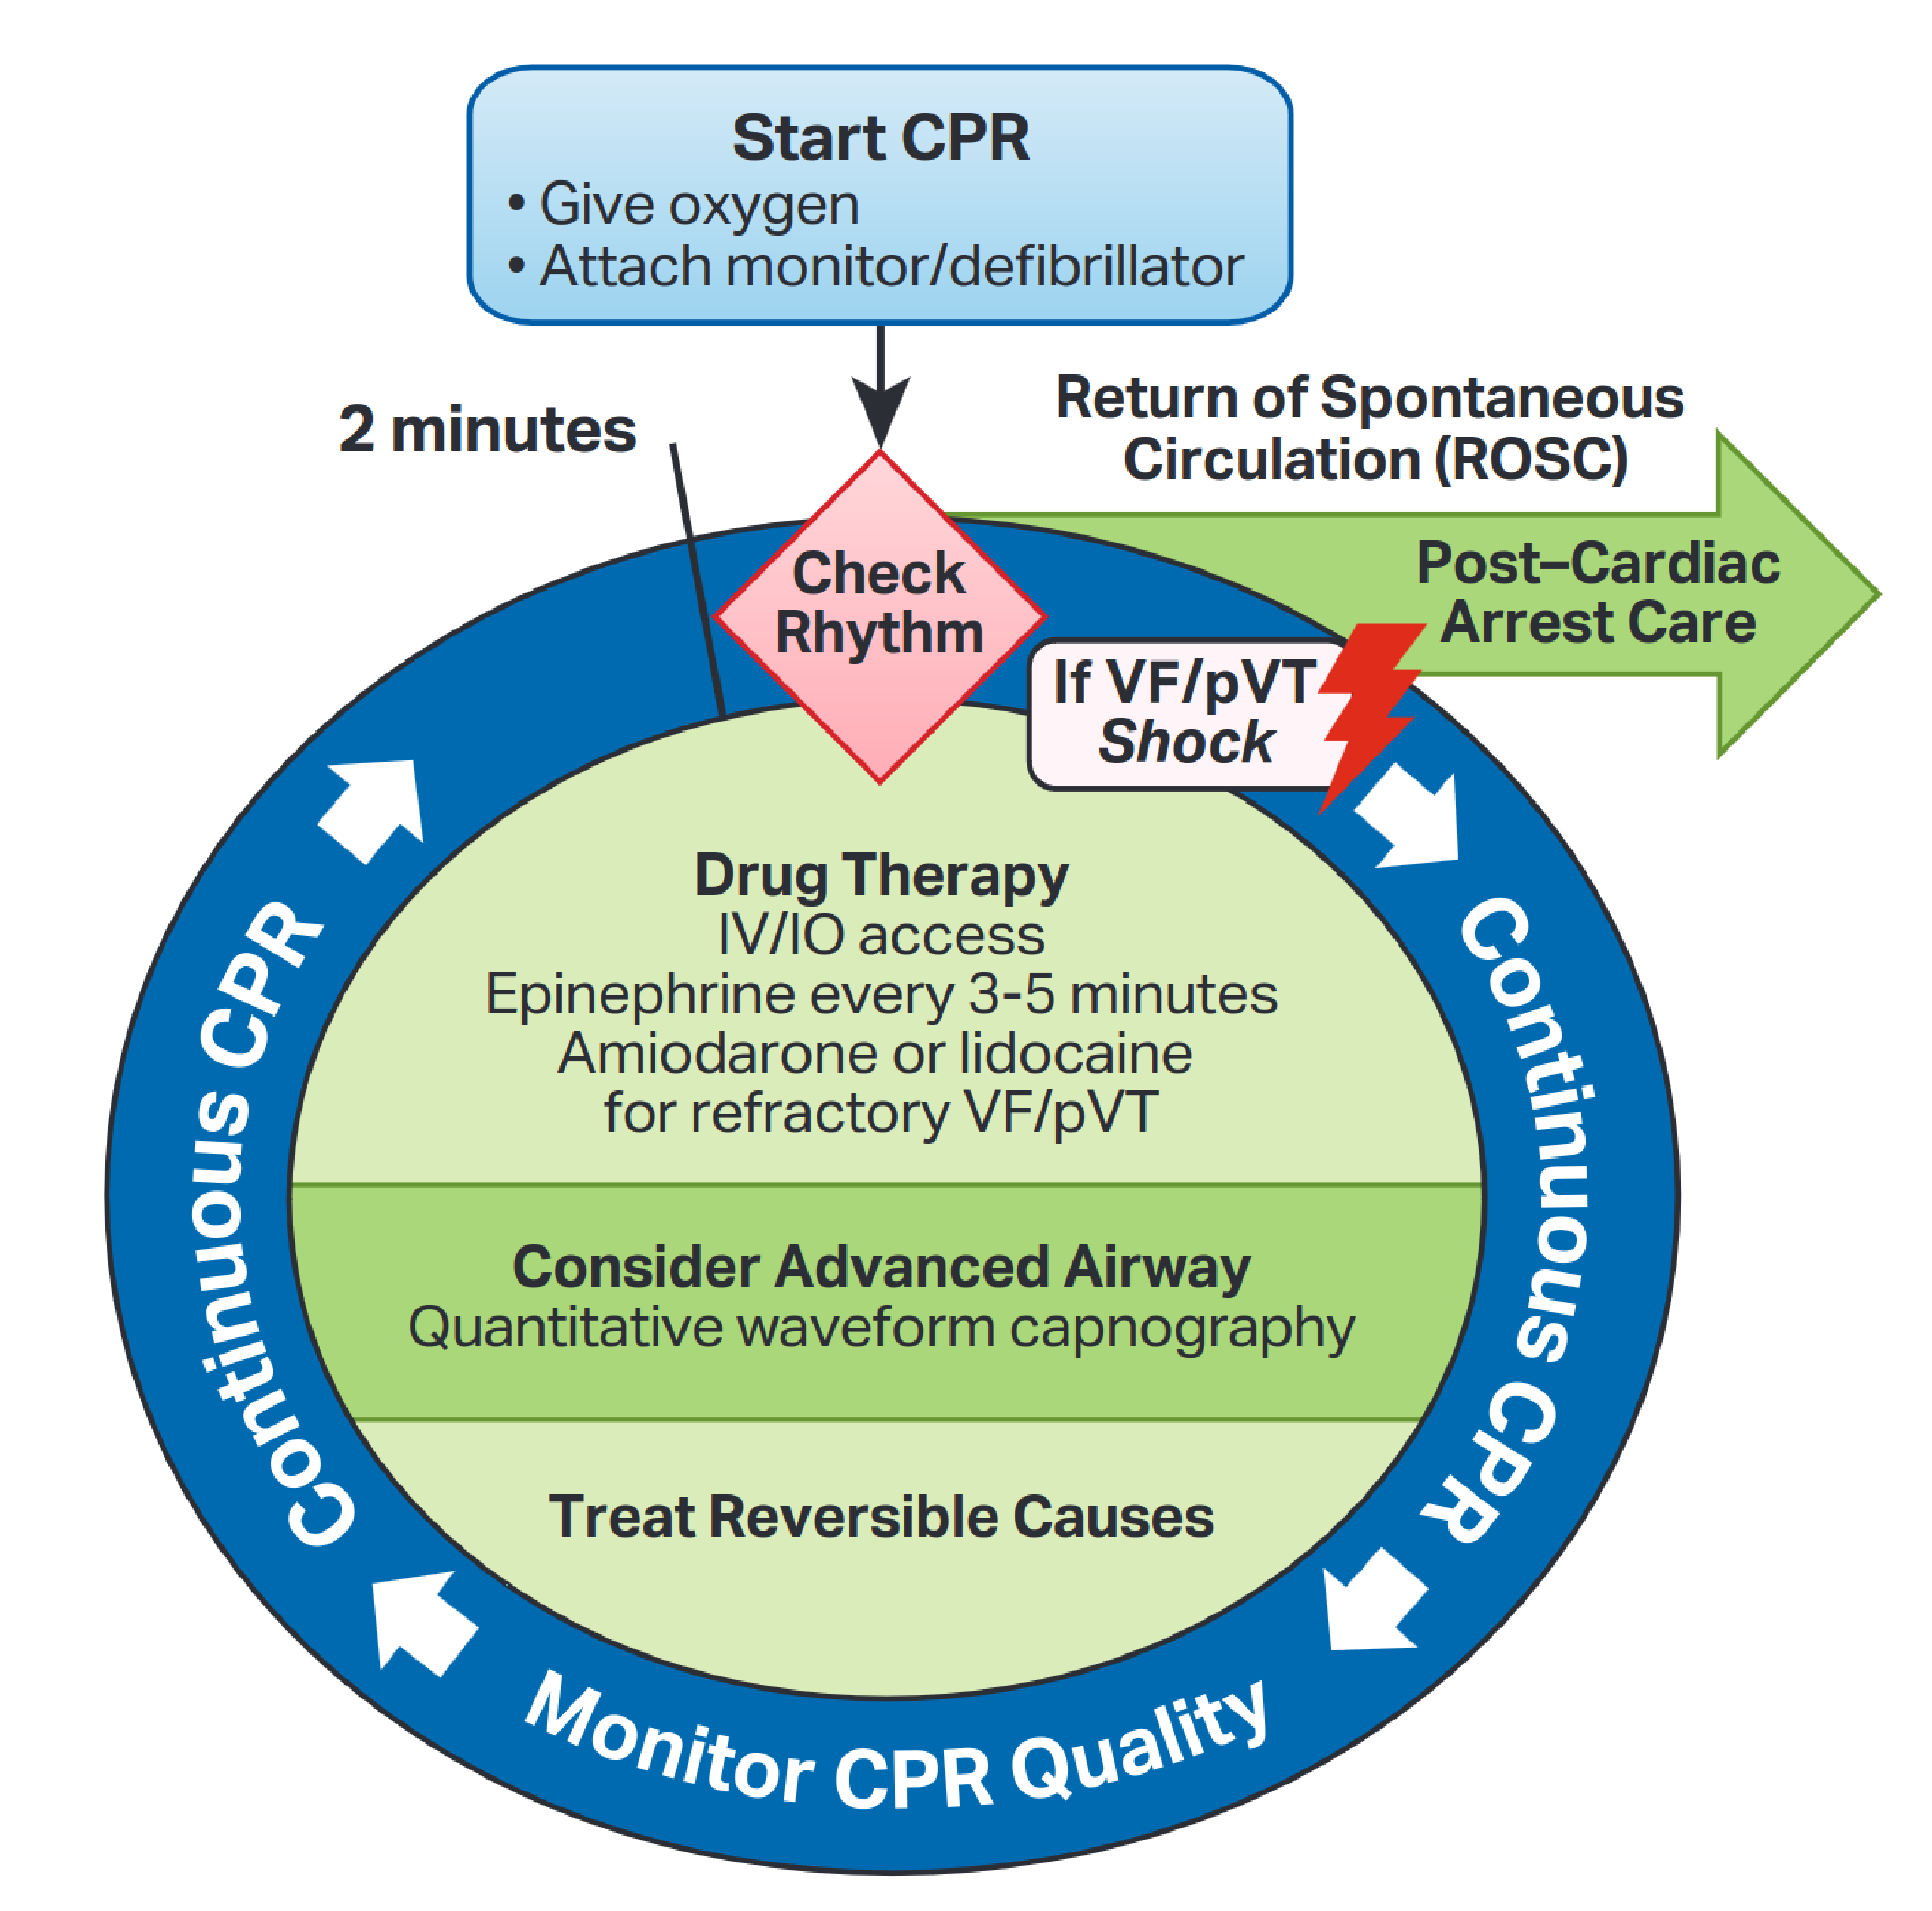
\includegraphics[width=0.5\textwidth]{acls-algorithm}
  \caption{Advanced Cardiac Life Support Guidelines}\label{fig:acls-algorithm}
\end{figure}

Advanced Cardiovascular Life Support (\ACLS{}) are a set of \BPGs{} periodically
published by the American Heart Association (\AHA{}) for management of
life-threatening cardiac conditions that will cause of have caused cardiac
arrest. The conditions that the guidelines treat range from dangerous arrhythmias, i.e.,
irregularities in heart's rhythm, to cardiac arrest---a cardiac emergency where
the heart stop pumping \cite{ACLSWikiEntry}.
The guidelines, according to the AHA{}, \say{are based on the most current
and comprehensive review of resuscitation science, systems, protocols, and
education} \cite{ACLSUrl}.

\autoref{fig:acls-algorithm} shows the \AHA{}'s guidelines for advanced
life support (\ACLS{}) for managing cardiac arrest in adults \cite{ACLSGuidelineUrl}.
\AHA{} publishes guidelines
for basic life support (\BLS{}), and pediatric counterparts of both. While
\BLS{} is meant for a first responder to provide treatment with
limited resources, such as an automatic emergency defibrillator (\AED{}),
\ACLS{} is supposed to be followed by teams of
trained professionals with advanced equipment for airway management,
drug delivery, etc.

\subsubsection{Why build \CDSSs{} for \ACLS{}?}

Cardiac arrest treatment is extremely time-critical, and outcomes
become significantly worse with every passing minute. This
gathering relevant data about the patient infeasible. Moreover, as
the seriousness of the condition necessitates multiple, simultaneous treatments
to be administered rapidly, intervention is usually executed following
standardized \ACLS{} algorithms \cite{ACLSWikiEntry}.

Prompt \ACLS{} guidelines-conformant treatment has been
shown to improve patient outcomes \cite{HonarmandResuscitation18}.
Moreover, deviations from the guidelines in in-hospital cases has been
associated with decreased rates of return of spontaneous circulation (\ROSC{}),
survival to discharge, and survival to discharge with favorable neurological
outcomes \cite{CrowleyResuscitation20}. Studies have also found that
inadequate \ACLS{} training can lead to poor retention, resulting
in reduced \ACLS{} conformance \cite{KiddJCN07}. Thus,
a \CDSS{} that can provide situation-specific guidance about
the next steps, especially in cases where \HCP{} training might be inadequate,
can potentially improve compliance, and consequently outcomes.

\subsubsection{A Brief Overview of Advance Life Support Guidelines for Cardiac Arrest:}

As we aren't concerned with intricacies of medical knowledge in the guideline,
we present a brief and simplified description of the guideline-prescribed treatment.
As \ACLS{} is supposed to be performed in settings where necessary equipment is
available, a electrocardiogram (EKG) machine is utilized to
monitor the patient's cardiac rhythm. Certain cardiac arrhythmias, characterized
by cardiac rhythms referred to as \emph{shockable}, must be treated
by delivering a therapeutic electric shock
\cite{DefibrillationWikiEntry}. As shown in \autoref{fig:acls-algorithm},
treatment has several parallel workflows such as:
\begin{itemize}
  \item Periodic monitoring of the cardiac rhythm, and in case of a
    \emph{shockable} rhythm, using a defibrillator.
  \item Continuous cardiopulmonary resuscitation (\CPR{}).
  \item Administration of vital drugs such as
    epinephrine every few minutes.
\end{itemize}
As \autoref{fig:acls-algorithm} suggests, these workflows must be
performed rapidly and periodically. As the duration of the intervention
is typically a few minutes, making optimal use of available time is critical to
outcomes.

\section{The \KACLS{} System}\label{sec:kacls-cdss}

\begin{figure}[t!]
  \centering
  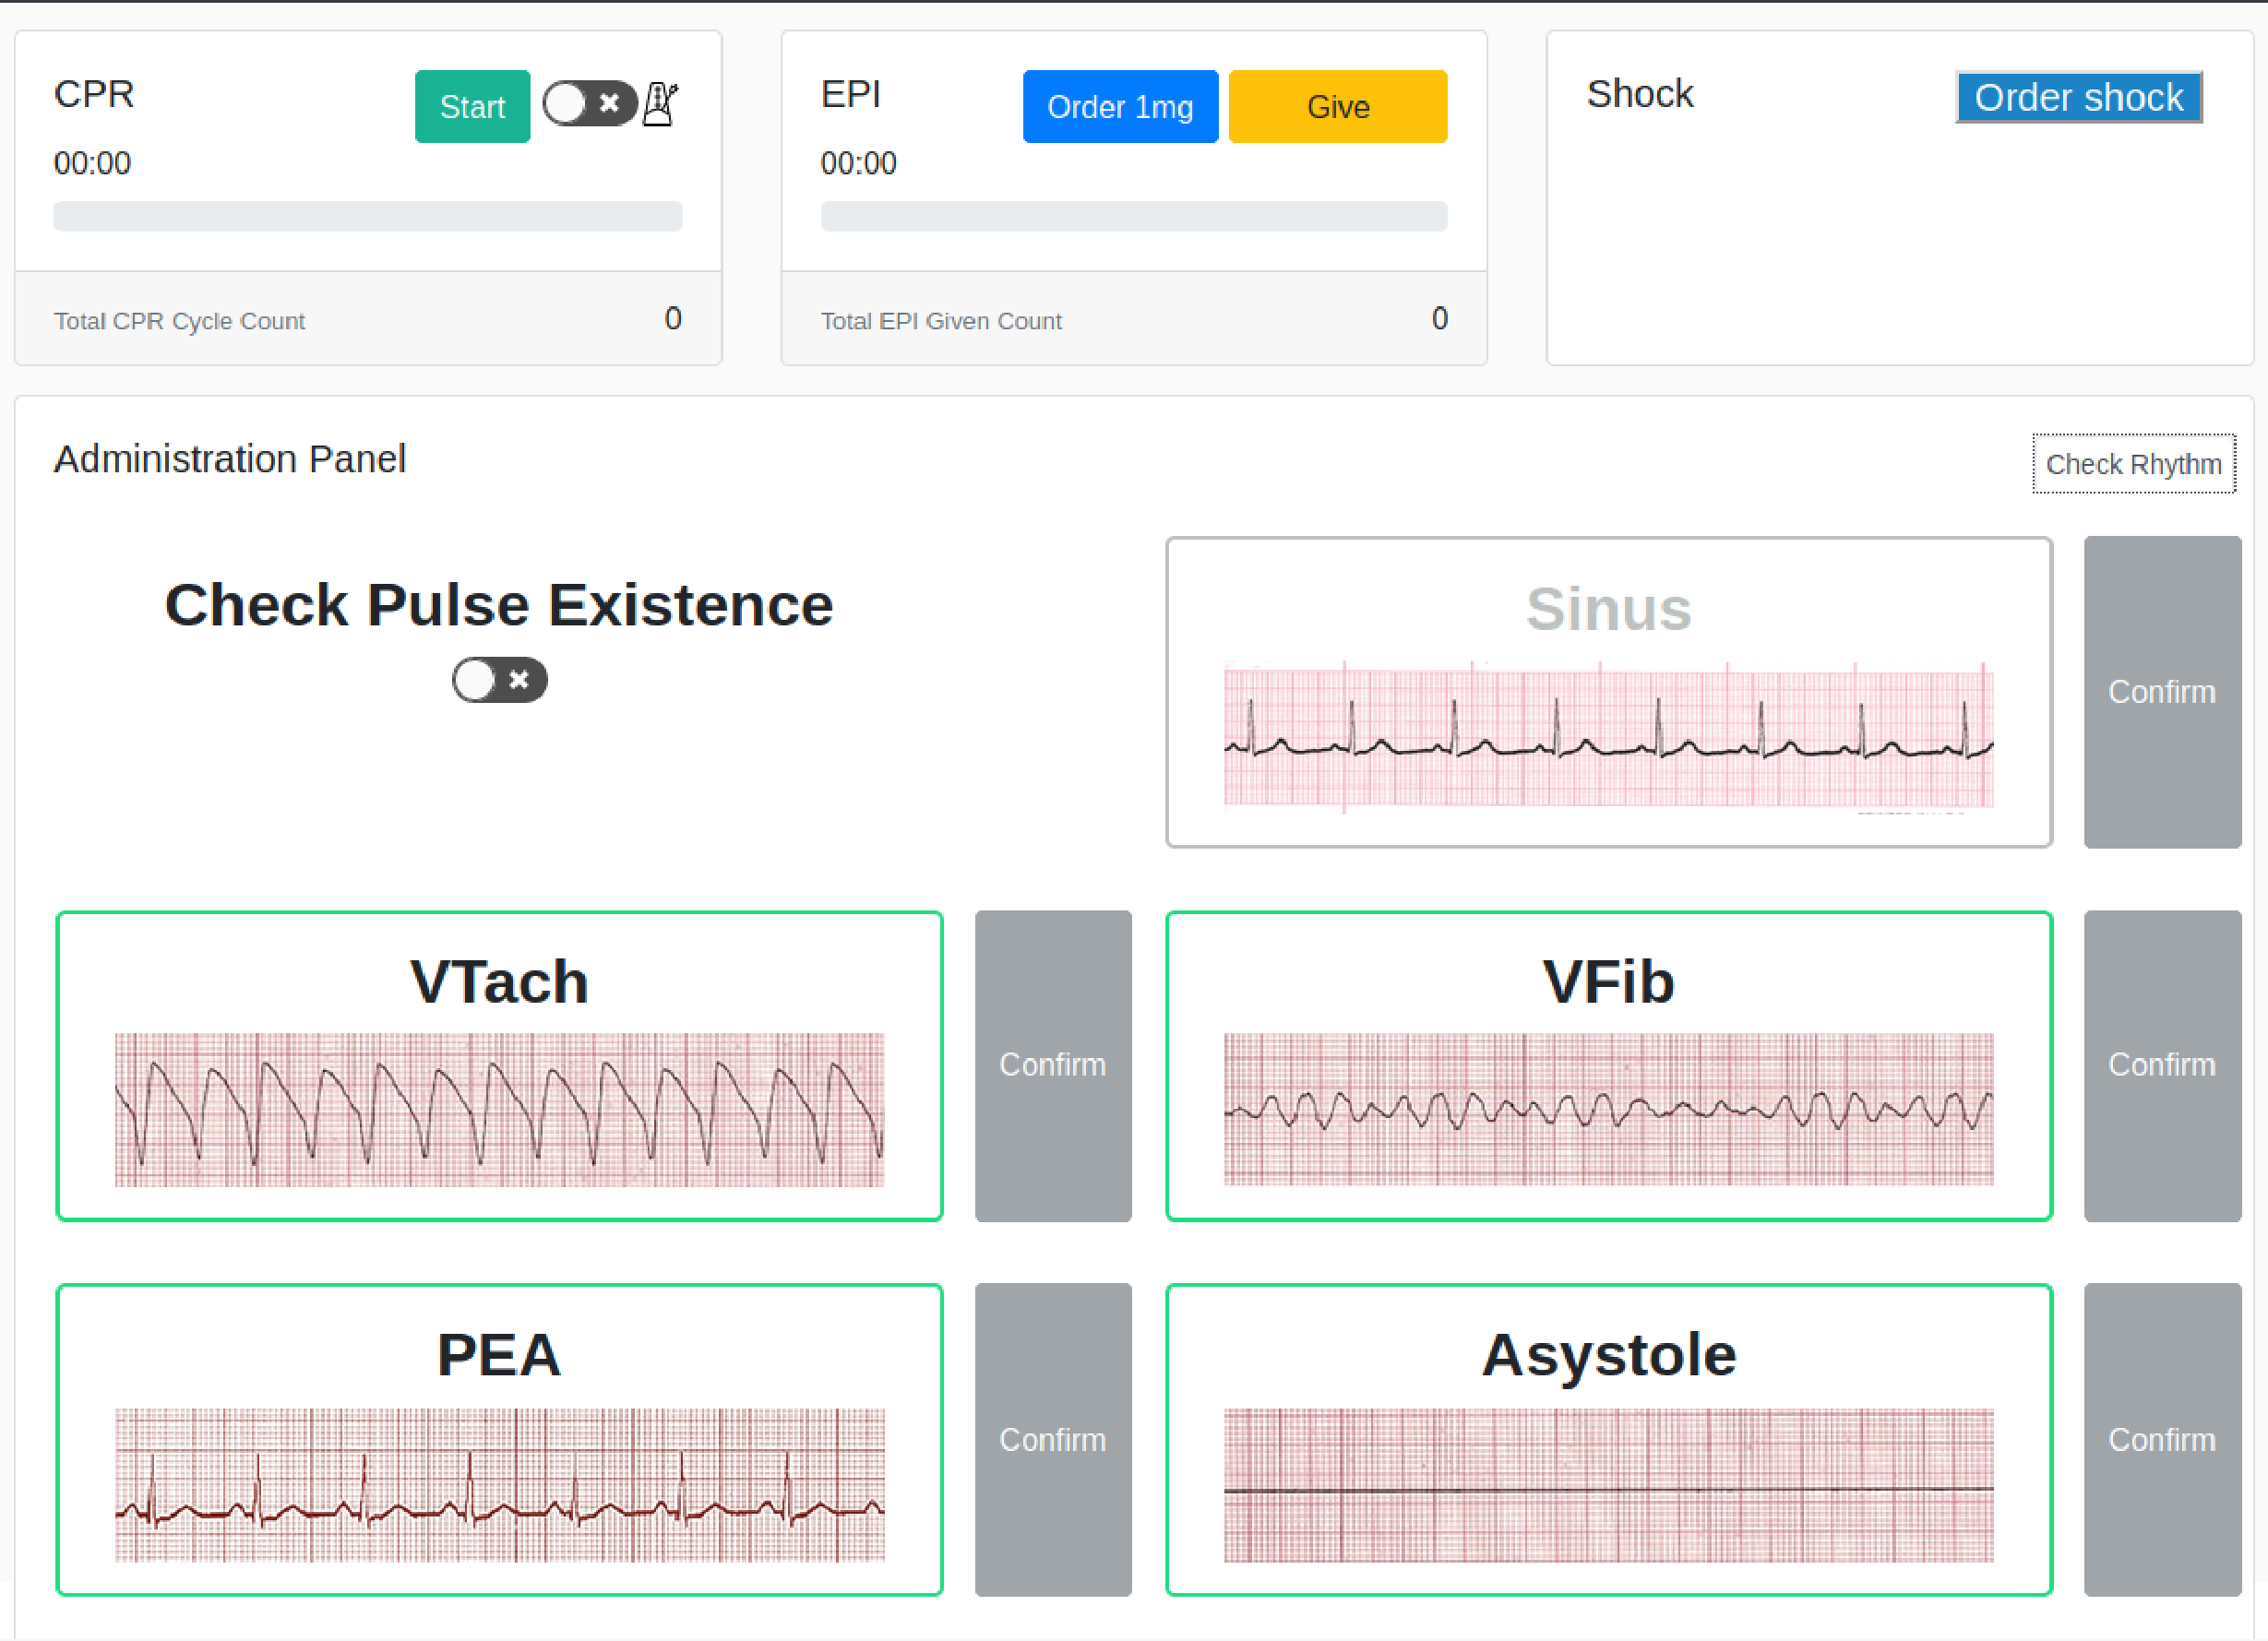
\includegraphics[width=0.85\textwidth]{acls-tool}
  \caption{Snapshot of \KACLS{}}\label{fig:kacls-snapshot}
\end{figure}

\autoref{fig:kacls-snapshot} shows a snapshot of our \CDSS{} for
enabling compliance to the advanced life support guidelines described in
\autoref{sec:acls}. Advanced life support is supposed to be performed by
a team of \HCPs{}, that take on roles such as a leader, \CPR{}-provider,
airway/respiratory specialist, Intravenous access (IV) and drug administration
specialist, pharmacist, defibrillator attendant and members that serve as
backups \cite{ACLSWikiEntry}. The leader is responsible for coordinating
treatment, our tool render support through a handheld tablet held by the leader.
\autoref{fig:kacls-snapshot} show a snapshot of said tablet's main screen.
Decision support, in the form of time-sensitive reminders, warnings when
procedures are stopped prematurely, or exceed stipulated limitations, and
confirmations regarding the patient rhythm's are provided on the screen
through popups and progress bars. For example, when the leader instructs
the team to start CPR, and presses the \say{Start} button under the \say{CPR}
section of the screen. A timer displays the duration and appropriate warnings
about prematurely stopping CPR or exceeding the time for a \CPR{} cycle are
displayed.

In \autoref{sec:modular-cdss-architecture}, we described
conceptual components of \CDSSs{}, and argued in favor
of developing \CDSSs{} using independently developed and maintained codebases
aligned with these components. The \KACLS{} system follows
this philosophy and has:
\begin{enumerate*}[label=(\roman*)]
  \item a simple \emph{frontend} written in Javascript using React \cite{ReactJSUrl} that handles
    user interaction, and,
  \item a $\K$-based HTTP server that encodes the \ACLS{} guideline
    and interacts with the frontend.
\end{enumerate*}
The use of the Javascript based frontend allows our application
to run on any modern web-browser. As shown in figure \ref{fig:kacls-snapshot},
our frontend consists of forms and buttons that correspond to procedures
in the algorithm in figure \ref{fig:acls-algorithm}. For example, the
\say{Start} button in the CPR box results in a two-minute timer corresponding
to the \say{2 minute continuous CPR} procedure in the informal description.
The frontend is simple and doesn't contain any guideline conformance related
logic. Interaction with the frontend simply results in dispatch of
\textit{events} to the backend. For example, when the \say{Start} button is pressed, a
\say{StartCpr} event is sent to the backend.


\subsection{Capturing Execution-specific Details}\label{sec:execution-specific-details}

A computer-interpretable version of a guidelines, unlike its
textual counterpart, may require specification of additional details
for execution. Such details can often be gathered from context in case
of textual guidelines or may be unintentionally missing. This was also
discussed in context of related approaches in \autoref{chapter:related-work},
especially in \autoref{sec:kiv-verification}.

As discussed in \autoref{sec:generic-bpg}, \BPGs{} can be notionally
represented using a collection of workflows. Each workflow has steps
executed sequentially but may be concurrently executed with steps from
other workflows. Consider the \ACLS{} guidelines discussed in
\autoref{sec:acls}. Several procedures, such as administering drugs,
and performing \CPR{} occur concurrently, where each procedure has
a set of tasks that need to be performed sequentially.
There may also be some implicit order across workflows, but we
address that in later chapters.

\subsubsection{Modeling \BPGs{} as State Machines}

In this work, we choose to express medical logic using
concurrently executing state machines with implicit queues for inter-machine communication.
Communicating state machines (\CSMs{}) is a well-understood model of concurrency
\cite{BrandJACM83} and is well-suited for representing medical guidelines in a
computer-interpretable format that is also \HCP{}-friendly.
We shall discuss the motivations behind using \CSMs{} in upcoming
chapters. For now, it suffices to describe how our choice addresses
issues mentioned in \autoref{sec:execution-specific-details}.
Given a guideline represented as a collection of workflows, we
describe each workflow via a state machine. The fact that
\CSMs{} can execute concurrently conveniently captures the
inherent concurrency in workflows.

\subsubsection{\ACLS{} Workflows as State Machines}

\begin{figure}[tb!]
\centering
\begin{subfigure}{\textwidth}
  \centering
  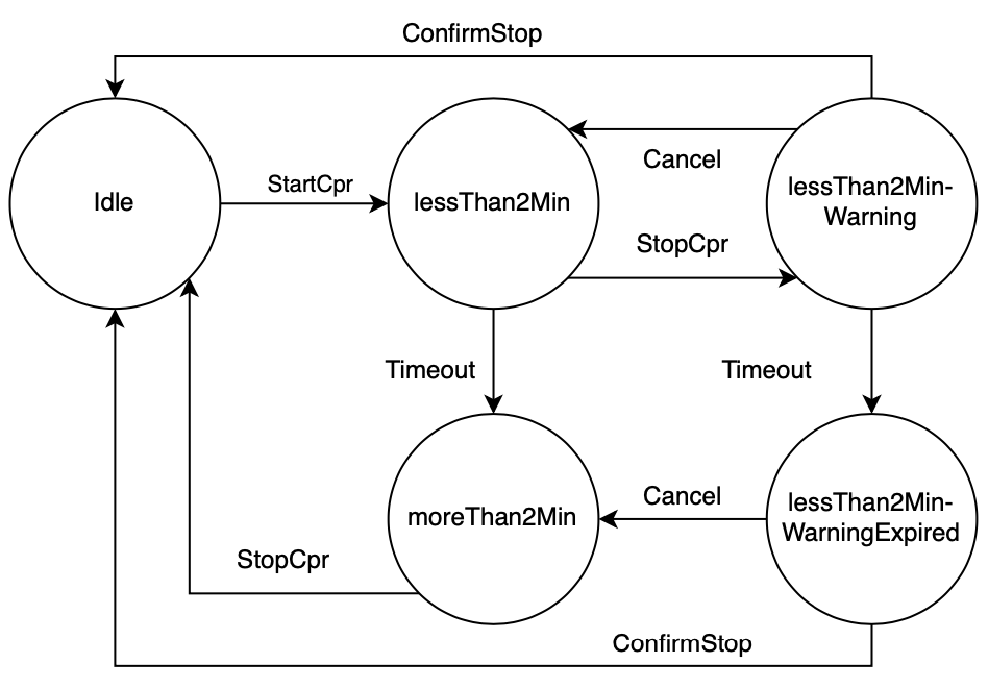
\includegraphics[width=0.55\linewidth]{cpr-machine}
  \caption{CPR Machine}
  \label{fig:cpr-machine}
\end{subfigure}%
\hfill\newline\hfill\newline\hfill
\begin{subfigure}{\textwidth}
  \centering
  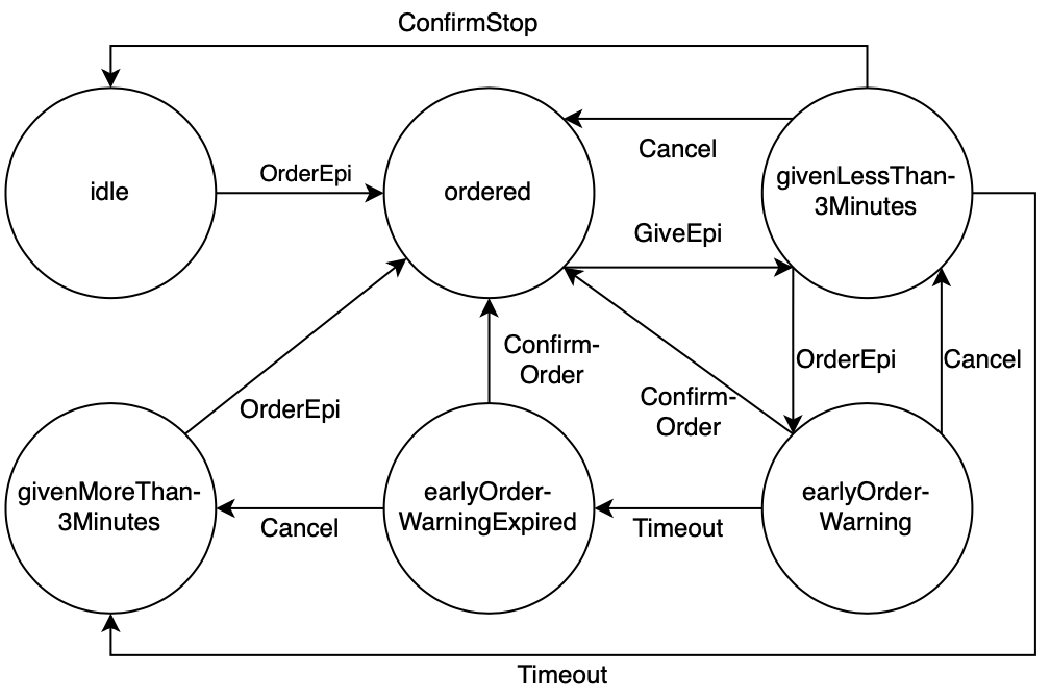
\includegraphics[width=0.55\linewidth]{epi-machine}
  \caption{Epinephrine Machine}
  \label{fig:epi-machine}
\end{subfigure}
\caption{Formal Machine Definitions}
\label{fig:machine-defs}
\end{figure}

At the start of \autoref{sec:kacls-cdss}, we mentioned that
the \emph{frontend} of our \CDSS{} is a simple Javascript-based
application to facilitate user interaction through buttons
and popups. We can now elaborate what we mean by \emph{simple}.
Button presses on the frontend correspond to \emph{events}
that trigger transitions in state machines shown in \autoref{fig:machine-defs}.
For instance, pressing the \say{Start} button under
the CPR part of the tool shown in \autoref{fig:kacls-snapshot} results in a
\inlinek{StartCPR} event that triggers the corresponding transition in
the machine in \autoref{fig:cpr-machine}.
Similarly, certain machine states result in events being dispatched
to the frontend that cause popups or messages to be displayed
on associated parts of the screen. Thus, the frontend itself contains
no medical logic.

\subsection{$\KACLS$ Backend}\label{sec:kacls-backend}

As described at the start of \autoref{sec:kacls-cdss},
the backend receives events from the frontend, processes them and
dispatches the results back to the frontend.
In \autoref{sec:execution-specific-details}, we described the
process of details required for execution by expressing
the \BPG{} using communicating state machines. For a functioning
backend through, we need to translate the abstract state machines
into an executable medium. We do this by encoding the
state machines in a $\K$ definition. Before we describe the
encoding, we describe some additional challenges that we need
to address in order to use $\K$ as a \CDSS{} backend.

\subsubsection{Additional Challenges}

\paragraph{Asynchronous External Communication:}
Communication with external process in \K{} is facilitated
by built-in I/O support. \K{} has built-in
functions for many operations that map directly to their
POSIX counterparts \cite{KFrameworkIOUrl}. However,
execution in $\K$ is single-threaded. Thus, to make \K{}
behave as an HTTP \cite{HTTPUrl} server that accept messages and respond asynchronously,
we need to write additional C++ initialization code and link it against
\K's LLVM backend \cite{KFrameworkBackendsUrl}.

\paragraph{Handling Timers:}
The \ACLS{} workflows shown in \autoref{fig:acls-algorithm} require
tasks being performed periodically. For instance, the algorithm
calls for continuous CPR administration for two minutes
between checking rhythm and performing defibrillation if needed.
Similarly drugs like epinephrine must be administered every three minutes.
\K{} does not support setting timers that can interrupt the \K{} process
on expiration. Thus, we rely on external \say{timers} that, instead
of interrupting the \K{} process, place a \inlinek{timeout} event
at the head of the \inlinek{<inputBuffer>} cell on expiration, which
trigger corresponding transitions in state machines. For example,
consider the CPR machine in \autoref{fig:cpr-machine}. When
\CPR{} is started through the press of a button on the frontend,
an external two-minute timer is set, and the machine
transition from state \inlinek{idle} to \inlinek{lessThan2Min}.
When the timer expires, the external timer sends a \inlinek{Timeout}
event to the \K{}, makes the \CPR{} machine to transition from
state \inlinek{lessThan2Min} to \inlinek{morethan2Min}.

\subsubsection{$\KACLS{}$ Backend}
Recall from \autoref{sec:semantics-in-k} that in $\K$ computation
is described via rewrite \emph{rules} that operate over a \emph{configuration}
that organizes data in labeled and potentially nested units called cells.
\autoref{lst:initial-configuration} shows the initial configuration for
the definition $\K$ of our state machines-based representation.
Note that unlike a typical $\K{}$ definition, the initial \inlinek{configuration}
does not have a \inlinek{<k>} cell containing a \inlinek{$PGM} variable
replaced by the program \AST{} at runtime, as the $\K$ definition is the
program itself.

\begin{lstlisting}[float=ht,
  frame=single,
  style=ksty,
  language=k,
  numbers=left,
  numbersep=5pt,
  caption={Initial Configuration},
  label={lst:initial-configuration},
  xleftmargin=3ex
]
configuration
    <machines>                                @\label{lstline:kacls-machines-cell-start}@
        <machine multiplicity="*" type="Set"> @\label{lstline:kacls-machine-cell-start}@
            <id>    .K   </id>
            <state> .K   </state>
            <store> .Map </store>
        </machine>                           @\label{lstline:kacls-machine-cell-end}@
    </machines>                              @\label{lstline:kacls-machines-cell-end}@
    <inputBuffer>  .JSONs </inputBuffer>     @\label{lstline:input-buffer-cell}@
    <outputBuffer> .JSONs </outputBuffer>    @\label{lstline:output-buffer-cell}@
\end{lstlisting}

Lines \ref{lstline:kacls-machines-cell-start}-\ref{lstline:kacls-machines-cell-end} declare
a cell \inlinek{<machines>} that will be used to multiple
\inlinek{<machine> ... </machine>} cells, declared between Lines
\ref{lstline:kacls-machine-cell-start} and \ref{lstline:kacls-machine-cell-end}, where
each cell stores all data related to a particular state machine. The
\inlinek{<id>} and \inlinek{<state>} cells store the machine's name and
active state respectively. The \inlinek{<store>} cell
is a map used to store any additional data. Note the following:
\begin{enumerate}[label=(\roman*)]
  \item The \inlinek{<machine>} cell is declared with an attribute
    \inlinek{multiplicity=*}, signifying that the configuration can contain
    multiple instances of such cells that are added or removed dynamically
    during execution. At the start of execution, the configuration has
    zero such cells.
  \item As the number of machines to represent is known and remains constant
    during execution, one might ask why they are not declared as a part of the
    initial configuration itself. We clarify that we deliberate not to do, due
    to reasons we explain shortly.
\end{enumerate}

Lines \ref{lstline:input-buffer-cell} and \ref{lstline:output-buffer-cell}
declare cells \inlinek{<inputBuffer>} and \inlinek{<outputBuffer>} respectively
that hold comma-separated lists of
JSON objects. As their name suggested, they are used as buffer to communicate with
the frontend. Incoming events from the
frontend are placed at the end of the \inlinek{<inputBuffer>} and outgoing
events intended for the frontend are consumed from head of the \inlinek{<outputBuffer>}.

\subsubsection{Initialization}

Initialization involves populating the configuration with the
initial state of each state machine. \autoref{lst:machine-initialization}
depicts the template of a rule for initializing machine
any machine \inlinekmath{$\mathcal{M}$}, with initial state \inlinek{u}.
Instead of starting \inlinek{<machines>} cell that is pre-populated with
\inlinek{<machine>} cells, we dynamically initialize
machines once the corresponding frontend component is rendered and ready.
When the frontend component associated with machine $\mathcal{M}$
is successfully loaded, it sends a \inlinekmath{"$\mathcal{M}$.init"} event,
which is added to the head of the input buffer.
For instance,  when the CPR part of the tool from
\autoref{fig:kacls-snapshot} has successfully loaded, it sends a \inlinek{"cprMachine.init"},
which is added to the head of the input buffer, where \inlinek{cprMachine} is
the name of the machine in the encoded \K{} definition, stored under the \inlinek{<id>} cell.
Lines \ref{lstline:machine-add-begin}-\ref{lstline:machine-add-end} of the rule
introduce a new \inlinek{<machine>} cell with name \inlinekmath{$\mathcal{M}$} and initial
state \inlinek{u}. The \inlinek{.Bag} in $\K$, seen on
\autoref{lstline:machine-add-begin}, represents the absence of a cell, which
the rule rewrites to a \inlinek{<machine>} cell, resulting in its
addition to the configuration under the \inlinek{<machines>} cell.
On \autoref{lstline:init-inputBuffer}, the $\K$ variable \inlinek{IN} matches any list of
JSON elements. Thus, \inlinekmath{"$\mathcal{M}$.init" , IN} matches any list with
\inlinekmath{"$\mathcal{M}$.init"} at the head of the list (\inlinek{IN} matches the tail of
the list). When the rule fires, the list is rewritten to
just the tail, resulting in the removal \inlinekmath{"$\mathcal{M}$.init"}
event from the \inlinek{<inputBuffer>} cell. For instance, in case of the CPR
machine, the initialization rule is show in \autoref{lst:cpr-init}.

%For instance, \autoref{lst:-initialization} shows the rule that initializes
%the CPR Machine to start in state \inlinek{idle} corresponding to the
%entry state of the machine in \autoref{fig:cpr-machine}.

\begin{lstlisting}[float=t!,
  mathescape=true,
  frame=single,
  style=ksty,
  language=k,
  numbers=left,
  numbersep=5pt,
  caption={Template For Machine Initialization Rule},
  label={lst:machine-initialization},
  xleftmargin=3ex
  ]
<machines>
  .Bag => ( <machine>                                      @\label{lstline:machine-add-begin}@
              <id> $\mathcal{M}$ </id>
              <state> u </state>
              ...
            </machine> )                                   @\label{lstline:machine-add-end}@
  ...
<machines>
<inputBuffer> $\mathcal{M}$.init, IN => IN </inputBuffer> @\label{lstline:init-inputBuffer}@
\end{lstlisting}


\begin{lstlisting}[float=h!,
  frame=single,
  style=ksty,
  language=k,
  caption={\inlinek{cprMachine} Initialization Rule},
  label=lst:cpr-init
  ]
<machines>
  .Bag => ( <machine>
              <id> cprMachine </id>
              <state> idle </state>
              ...
            </machine> )
  ...
<machines>
<inputBuffer> cprMachine.init, IN => IN </inputBuffer>
\end{lstlisting}

For each machine $\mathcal{M}$ in the guideline, the $\K$ definition
contains a corresponding rule of the form shown in
\autoref{lst:machine-initialization} in the definition. Next,
we discuss each machine in detail to explain how we encode
their transition systems in $\K$.

\subsubsection{CPR Machine}

The \textit{CPR Machine} encodes the intended CPR procedure
shown in figure \ref{fig:cpr-machine}. As mentioned earlier, when the user clicks
the \say{Start} button in the CPR pane in figure \ref{fig:kacls-snapshot},
an external two-minute timer is started. If the user decides to stop CPR before
two minutes are up, a message is displayed to the user warning him of
deviation from the intended guidelines. If the user stops CPR after
two minutes, no warning message is displayed.
\autoref{lst:cpr-machine-start} shows the rule that
fires when the \say{Start} button in clicked.
The rule does the following:
\begin{enumerate}[label=(\alph*)]
  \item Consumes the \inlinek{"StartCpr"} event from the \inlinek{<inputBuffer>} in
    \autoref{lstline:read-inputBuffer}.
  \item Move the machine from state \inlinek{idle} to state \inlinek{lessThan2Min}
    in \autoref{lstline:idle-lessThan2Min}.
  \item Sends a \inlinek{startTimer} action to the frontend via the
    \inlinek{<outputBuffer>} (encoded as JSON) in
    Lines \ref{lstline:external-timer-start-begin}-\ref{lstline:external-timer-start-end},
    which results in the start of a two-minute timer in the frontend.
\end{enumerate}
Note how features of $\K$ discussed in \autoref{sec:k-framework}
make the definition \emph{concise} yet \emph{descriptive}. Specifically:
\begin{itemize}
  \item The \emph{configuration abstraction} mechanism enables only parts of the
  configuration that are not used in the rule to be easily ignored.
    The \inlinek{...} (dots) on
    \autoref{lstline:machine-abstraction-dots} contents of cell
    not used in the rule to be safely ignored. Other parts
    of the configuration, such as the \inlinek{<machines>} cell
    and the \inlinek{<outputBuffer>} cell need not be mentioned at all.
  \item Localized rewriting enables the rewrite symbol \inlinek{=>} to
    apply on deeply nested subterms. This enables de-duplication,
    as parts of the term that remain unchanged don't have to be
    specified both on the \LHS{} and \RHS{} of the rewrite. For instance,
    the \inlinek{<store>} cell on \autoref{lstline:store-abstraction-dots}
    contains is a map that holds information about the machine, such as
    execution status. Recall that a map with $n$ key-value pairs is
    depicted in $\K$ as
    \inlinekmath{($k_1$ |- $\ v_1$), ($k_2$ |- $\ v_2$), $\dots\ $, ($k_n$ |- $\
    v_n$)}. Localized rewriting enables us to only rewrite the
    value mapped to key \inlinek{"cprRunning"} from any value
    to \inlinek{true} and ignore other parts of the map using \inlinek{...}
    notation.
\end{itemize}
\begin{lstlisting}[float=t,
  frame=single,
  style=ksty,
  language=k,
  numbers=left,
  numbersep=5pt,
  caption={CPR Machine in \K{}},
  label={lst:cpr-machine-start},
  xleftmargin=3ex
]
rule <machine>
          <id> cprMachine </id>
          <state> idle => lessThan2Min </state>                    @\label{lstline:idle-lessThan2Min}@
          <store> ( "cprRunning" |-> (_ => true) ) ... </store>    @\label{lstline:store-abstraction-dots}@
          ...                                                      @\label{lstline:machine-abstraction-dots}@
     </machine>
     <inputBuffer> "StartCpr" , IN => IN </inputBuffer>            @\label{lstline:read-inputBuffer}@
     <outputBuffer>                                                @\label{lstline:external-timer-start-begin}@
         OUT => OUT +JSONs jsonResponse( cprMachine
                                       | lessThan2Min
                                       | startTimer( .JSONs ) )
     </outputBuffer>                                               @\label{lstline:external-timer-start-end}@
\end{lstlisting}

\subsubsection{Epinephrine Machine}
\begin{lstlisting}[float=h,
  frame=single,
  style=ksty,
  language=k,
  numbers=left,
  numbersep=5pt,
  caption={Epi Machine in $\K$},
  label={lst:epi-machine-rule},
  xleftmargin=3ex
]
rule <machine>
      <id> epiMachine </id>
      <state> givenLessThan3Min
          => earlyOrderWarningNotification
      </state>
      <store> .Map => ("tentativeOrder" |-> ORDERED) ... </store>
    </machine>
    <inputBuffer> { "event" : "orderEpi"                              @\label{lstline:input-buffer-json-read-begin}@
                  , "data"  : [ ORDERED:Int ] } , IN
              => IN
    </inputBuffer>                                                    @\label{lstline:input-buffer-json-read-end}@
    <outputBuffer> OUT                                                @\label{lstline:output-buffer-warning-begin}@
      => OUT +JSONs jsonResponse( epiMachine
                                | earlyOrderWarningNotification
                                | showEarlyOrderWarning( .JSONs ))   @\label{lstline:output-buffer-warning-end}@
    </outputBuffer>
\end{lstlisting}

The \textit{Epinephrine Machine} encapsulates instructions for administering
the drug Epinephrine to the patient. The corresponding machine is shown in figure
\ref{fig:epi-machine}. The user orders the drug using the
\say{Order 1mg} button and can administers it using the \say{Give} button in
Epinephrine pane in figure \ref{fig:kacls-snapshot}. Giving the drug results in the
start of a three-minute timer, during which if a new order is placed, a warning
is issued.

\begin{lstlisting}[float=b!,
  frame=single,
  style=ksty,
  language=k,
  label={lst:general-rewrite},
  caption={Transitions as $\K$-Rules}
]
  <machine>
    <id> @$\mathcal{M}$@ </id>
    <state> @$u$@ => @$v$@ </state>
    ...
    <machine>
  <inputBuffer> @$\sigma$@, IN => IN </inputBuffer>
\end{lstlisting}

\autoref{lst:epi-machine-rule} encodes the transition
$\textssf{givenLessthan3Min} \xrightarrow[]{\textssf{orderEpi}}
\textssf{earlyOrderWarningNotification}$ from \autoref{fig:epi-machine}.
The rule fires when it has been less than three minutes
before the last dose and a fresh order for
Epinephrine is put in (Lines
\ref{lstline:input-buffer-json-read-begin}-\ref{lstline:input-buffer-json-read-end}).
Note that the input event here also has a payload corresponding to the dosage,
depicted by a JSON object with fields \inlinek{"event"} for the event's name
and \inlinek{"data"} for the dosage.
As the guidelines dictate that Epinephrine must be administered
every three minutes, ordering fresh Epinephrine is a deviation from the
guidelines. Thus, an appropriate warning message is presented to the user (Lines
\ref{lstline:output-buffer-warning-begin}-\ref{lstline:output-buffer-warning-end}).

\subsubsection{Encoding Remaining Transitions}

Note that we only show a single rule from the \textit{CPR} and
\textit{Epinephrine} Machines as other rules resemble the ones
shown, and have a one-to-one correspondence to transitions in the
state machines in \autoref{fig:machine-defs}. For instance,
the rule in \autoref{lst:cpr-machine-start} encodes the transition
``$\textssf{idle} \xrightarrow[]{\textssf{StartCpr}} \textssf{lessThan2Min}$'' in the
CPR state machine in \autoref{fig:cpr-machine}. To encode the entire machine,
along with the initialization rule,
we encode every transition $u \xrightarrow[]{\sigma} v$
of machine $\mathcal{M}$ as a rewrite rule of the form shown in
\autoref{lst:general-rewrite}

\begin{lstlisting}[float=b!,
  frame=single,
  style=ksty,
  language=k,
  numbers=left,
  numbersep=5pt,
  caption={Shock Machine in $\K$},
  label={lst:shock-machine},
  xleftmargin=3ex
]
rule <machine>
        <id> shockMachine </id>
        <state>
          shockableRhythm => checkRhythm                         @\label{lstline:shock-state}@
        </state> ...
      </machine>
      <machine>
        <id> cprMachine </id>
        <store> ( "cprRunning" |-> false ) ... </store> ...      @\label{lstline:cpr-false}@
      </machine>
      <machine>
        <id> epiMachine </id>
        <store> ( "epiGiven" |-> true ) ... </store> ...        @\label{lstline:epi-true}@
      </machine>
      <inputBuffer> "administerShock" , IN => IN </inputBuffer>
      <outputBuffer> OUT                                        @\label{lstline:shock-response-begin}@
      => OUT +JSONs jsonResponse( shockMachine
                                | checkRhythm
                                | confirmShock("CPR for
                                                2 Minutes" ) )  @\label{lstline:shock-response-end}@
      </outputBuffer>
\end{lstlisting}

\subsubsection{Shock Machine}

We now describe the \textit{Shock Machine}. Intuitively, this
machine ensures:
\begin{enumerate*}[label=(\alph*)]
  \item shocks are only administered if the rhythm is shockable,
  \item CPR is administered every two minutes, and,
  \item drugs (such as Epinephrine) are periodically administered.
\end{enumerate*}
In case the of deviation appropriate warnings are issued. The \textit{Shock}
machine differs from other machines, as its transitions depend
on the status of both the \textit{CPR} and \textit{Epinephrine} machines.

\autoref{lst:shock-machine} shows a rule from the \textit{Shock} machine.
The rule fires when the rhythm is \textit{shockable}, and the user
wants to administer a shock. Additionally, CPR hasn't been administered
(\autoref{lstline:cpr-false}), but
Epinephrine has been administered (\autoref{lstline:epi-true}).
In such a situation, the user is informed that it is safe to
administer a shock, which should be followed by
two minutes of CPR (Lines
\ref{lstline:shock-response-begin}-\ref{lstline:shock-response-end}).
However, it is not safe to assume that the rhythm would remain
\textit{shockable} for subsequent shocks. Thus, the machine moves from
state \inlinek{shockableRhythm} to \inlinek{checkRhythm}. If the
user tries to administer another shock, a prompt to confirm the rhythm will be
displayed to ensure a shock is not administered in case of an \emph{unshockable}
rhythm.

We draw the user's attention to the \textit{succinctness} and \textit{simplicity}
of the rule. Despite expressing the interaction between three different machines,
$\K$'s configuration abstraction mechanism ensures that only relevant parts of
each machine are mentioned, making the transition \textit{comprehensible}.

\section{Discussion}\label{sec:rewriting-based-guidelines-discussion}

This chapter describes the process of systematically encoding
\BPGs{} expressed using informal flowchart-like notations as communicating
state machines (\CSMs{}). The \CSMs{} can then be encoded in a $\K{}$,
where, for every machine, $\mathcal{M}$, every transition
$u \xrightarrow[]{\sigma} v$
can be encoded as a rewrite rule of the form shown in
\autoref{lst:general-rewrite}. We discussed how
\emph{configuration abstraction}, \emph{localized rewriting} and
the inherent concurrency of rewriting enable the $\K$ encoding of
the guideline to be both \textit{succinct} and \textit{simple}.
But, comprehending such $\K$ based guidelines precludes comprehending
the $\K$ language, which is unreasonable to expect not only from domain
experts in medicine, but also from software developers in general.
The $\K$ language is designed for development and implementation of
programming languages, and can have an associated learning curve, especially
if one is unfamiliar with the theory of defining formal semantics.
Thus, understanding \K{} may require additional effort
for most software developers, who are more comfortable with
popular general purpose programming languages such as Java, C and python.
Moreover, the $\K$ definition can become harder to comprehend as
more complex guidelines are modeled, requiring rules that encode
transitions where multiple steps must be performed and complex
conditions to determine when the transitions can occur.

In upcoming chapters, we address shortcomings of using $\K$ directly
to model guidelines by coming up with a novel \DSL{} specifically
designed to encode medical logic. This language, called $\MediK{}$,
differs from $\K$ in many aspects. Notably $\MediK$:
\begin{itemize}
  \item Uses syntax that borrows from other languages for \CSMs{}, notably P
    \cite{DesaiPLDI13}, to improve comprehensibility and readability, albeit at
    the expense of succinctness.
  \item Provides support for interacting with heterogeneous external devices,
    such as monitors, patient sensors, etc.
\end{itemize}

\chapter{\MediK{}: Towards Safe Guidelines-based \CDSSs{}}\label{chapter:medik-safe-cdss}

In \autoref{chapter:k-based-guidelines}, we discussed the process
of encoding best practice guidelines (\BPGs{}) as \K{} definitions
to describe a systematic way of building \CDSSs{}. Specifically,
we described the process of encoding medical knowledge in guidelines
notionally via workflows that can be expressed abstractly as
concurrently executing finite state machines that communicate
via passing messages. Next, we described the process of
expressing state machines as \K{} definition, where \K{} features
such as configuration abstraction and local rewriting
enable \emph{conciseness}. We then combined the \K{} definition
with a simple javascript-based frontend to develop a \CDSS{}
for assisting healthcare practitioners (\HCPs{}) follow the
Advanced Life Support (\ALS{}) guidelines for managing
cardiac arrest published by the American Heart Association.

In \autoref{chapter:hurdles-cdss-adoption}, we described
that wider \CDSS{} adoption is incumbent on a having a
systematic way of developing guidelines with validated
content. The approach described in \autoref{sec:semantics-first}
attempts to enable such a way. It dictates that:
\begin{enumerate*}[label=(\roman*)]
  \item the semantics of the language be formally defined, from
  which tools are derived from a correct-by-construction fashion, and,
  \item ensuring that semantics of medical knowledge is accurately
  described.
\end{enumerate*}
As is typically the case, the \KACLS{} system from
\autoref{sec:kacls-cdss} through collaboration between
\HCPs{} and computer scientists. While the \K{}-based
representation of the \ALS{} guideline was concise,
it was not easily comprehensible to \HCPs{}, or to other
software engineers without prior experience of using \K{}.
This chapter addresses limitations of our work from
\autoref{chapter:k-based-guidelines}. Specifically, we describe
\MediK{} (pronounced \say{Medi-kay} \footnote{\MediK{} is a portmanteau of
Medicine and \K}) a novel domain-specific language (\DSL{}) for
expressing medical knowledge that is designed from the ground-up
with \HCP{}-comprehensibility in mind. As the name suggest, \MediK{}
has a formal $\K$ semantics, from which all tools for it are derived,
including its interpreter. \MediK{} has been used to implement a
complex \CDSS{} for management of sepsis in pediatric cases that
has multiple concurrent workflows. Our \MediK-based system has
been shown to satisfy desired safety properties, and to the
best of our knowledge, is the first such system with formal safety
guarantees.

The rest of this chapter is organized as follows. In \autoref{sec:sepsis-bpg}
we recall the example \BPG{} from section \autoref{sec:bpg-background}
for management of sepsis, to illustrate common requirements
that \DSL{} for modeling \BPGs{} should satisfy.
In \autoref{sec:medik}, we introduce the \MediK{} \DSL{}, and illustrate how
it has been specifically designed to address said requirements.
In \autoref{sec:evalution}, we evaluate the effectiveness of our approach
by utilizing it to build a \CDSSs{} intended for real-world use.
In section \autoref{sec:discussion}, we discuss how \MediK{} builds on
existing approaches in \autoref{chapter:related-work} to advance the
state-of-art in addressing challenges from \autoref{chapter:hurdles-cdss-adoption}.


\section{Pediatric Sepsis Management \BPG{}}\label{sec:sepsis-bpg}

In \autoref{sec:bpg-background}, we presented a best practice
guideline for management of sepsis in pediatric cases.
We briefly describe the guidelines here. Recall that
sepsis is life-threatening condition caused by the body's extreme response to
an infection, and is a major cause of morbidity and mortality
in children. Evidence indicates that timely
identification and prompt treatment with antibiotics and
intravenous (IV) fluids is \emph{vital} for avoiding
adverse outcomes \cite{Weiss2014CCM,Evans2018JAMA}.
The \BPG{} has several concurrent workflows with inter-workflow
dependencies, making it suitable to study common characteristics of \BPGs{},
which we recall here. Specifically, \BPGs{}:
\begin{itemize}
  \item Involve \stress{concurrent} workflows, such as administering drugs,
    monitoring vitals, performing treatment, etc. There may also be
    inter-workflow interactions. For instance, a diagnosis of sepsis during the
    screening may require modifications to an ongoing course antibitiotics.
  \item Often specified in a \stress{flowchart-like}
    notation. See \cite{AHAFlowcharts} and \cite{CancerCareFlowcharts} for other flowchart-based \BPGs{} for management of \emph{cardiac arrest}, and
    screening, risk-reduction, treatment and survivorship in
    cancer care respectively.
  \item Require communication between \stress{heterogeneous agents} such as
     monitors and Electronic Health Records (EHRs).
  \item Often use \stress{tables} indexed by parameters such as age, weight,
    etc to present normal/abnormal ranges for measurements, or recommended dosages for drugs.
\end{itemize}
%While section
%\autoref{sec:bpg-background} briefly discussed some sepsis workflows, here
%we discuss remaining workflows and their interdependencies in detail.

%Recall from \autoref{sec:bpg-background} that once sepsis has been detected,
%it is treated by administering fluids and antibiotics.
%Additionally, sepsis
%lead to septic shock---a condition characterized by acute cardiovascular
%distress.

%Adverse outcomes can, however, be mitigated through timely
%identification and prompt treatment with antibiotics and
%intravenous (IV) fluids \cite{Weiss2014CCM,Evans2018JAMA}.
%\BPGs{} for screening and management of sepsis in pediatric Emergency
%Departments (EDs) have shown effectiveness in screening and management of sepsis \cite{Eisenberg2021JP},
%leading to their adoption in many pediatric EDs \cite{Balamuth2017EM,Sepanski2014FP}.
%
%In \figurename{} \ref{fig:sepsis-screening}, we present a simplified version of
%the screening section of OSF's sepsis mangement guideline.
%In essence, when a patient arrives at the
%\ED{} with a fever or an infection, the \HCP{} is supposed to obtain
%\begin{enumerate*}[label=(\alph*)]
%  \item the patient's age,
%  \item any conditions, such as cancer, immunosuppresssion, etc,
%    that increase likelihood of sepsis, and
%  \item the patient's vital signs, such as heart rate, systolic blood
%    pressure, respiratory rate, etc.
%\end{enumerate*}
%\begin{footnotesize}
%  \begin{table}
%    \centering
%    \begin{tabular}{ | c || c | c | c | }
%      \hline
%      \textbf{Age}            & \textbf{Heart Rate}   & \textbf{Systolic BP} & \textbf{Temp}  \\
%      \hline
%      $0d - 1m$               & $>205$                & $<60$                & $<36 \text{ or } >38$ \\
%      \hline
%      $\geq 1m - 3m$          & $>205$                & $<70$                & $<36 \text{ or } >38$ \\
%      \hline
%      $\geq 3m - 1y$          & $>190$                & $<70$                & $<36 \text{ or } >38.5$ \\
%      \hline
%      $\dots$                 & $\dots$               & $\dots$              & $\dots$ \\
%      \hline
%      $\geq 13y$              & $>100$                & $<90$                & $<36 \text{ or } >38.5$ \\
%      \hline
%    \end{tabular}
%    \caption{Vital Signs Chart}\label{table:vital-signs}
%  \end{table}
%\end{footnotesize}
%
%This information is then used to check for abnormalities
%in clusters of linked information, called \say{buckets}. For instance, if
%the patient's heart rate is abnormal, then \say{bucket 1} is said to
%have an abnormal value.
%Checking for such abnormalities often involves the use of tables, such as
%\tablename{} \ref{table:vital-signs} that contains normal ranges indexed by
%\emph{age}.
%%\footnote{For brevity, we omit some age ranges and vital signs from table
%%\ref{table:vital-signs}}.
%If the patient has at least one abnormal value in every \say{bucket},
%then he/she is flagged as potentially septic.
%
%The \BPG{}-recommended treatment for
%sepsis involves multiple concurrent workflows, such as
%screening for septic shock, fluid resuscitation, and administering antibiotics.
%In \figurename{} \ref{fig:fluid-therapy}, we provide
%a version of the fluid resuscitation guideline used
%at OSF. Briefly, if the patient is flagged as potentially septic, the guideline suggests
%\begin{enumerate*}[label=(\roman*)]
%  \item obtaining any fluid-overload risks,
%  \item administering normal saline (typically over a period of 15 minutes),
%    where the dosage is dictated by risks determined in previous step,
%  \item assessing signs of fluid-overload,
%  \item evaluating patient responsiveness to normal saline upon completion of
%    the administering process, and,
%  \item determining whether another fluid bolus should be administered based on
%    information from previous steps.
%\end{enumerate*}
%\begin{figure}[b]
%  \centering
%  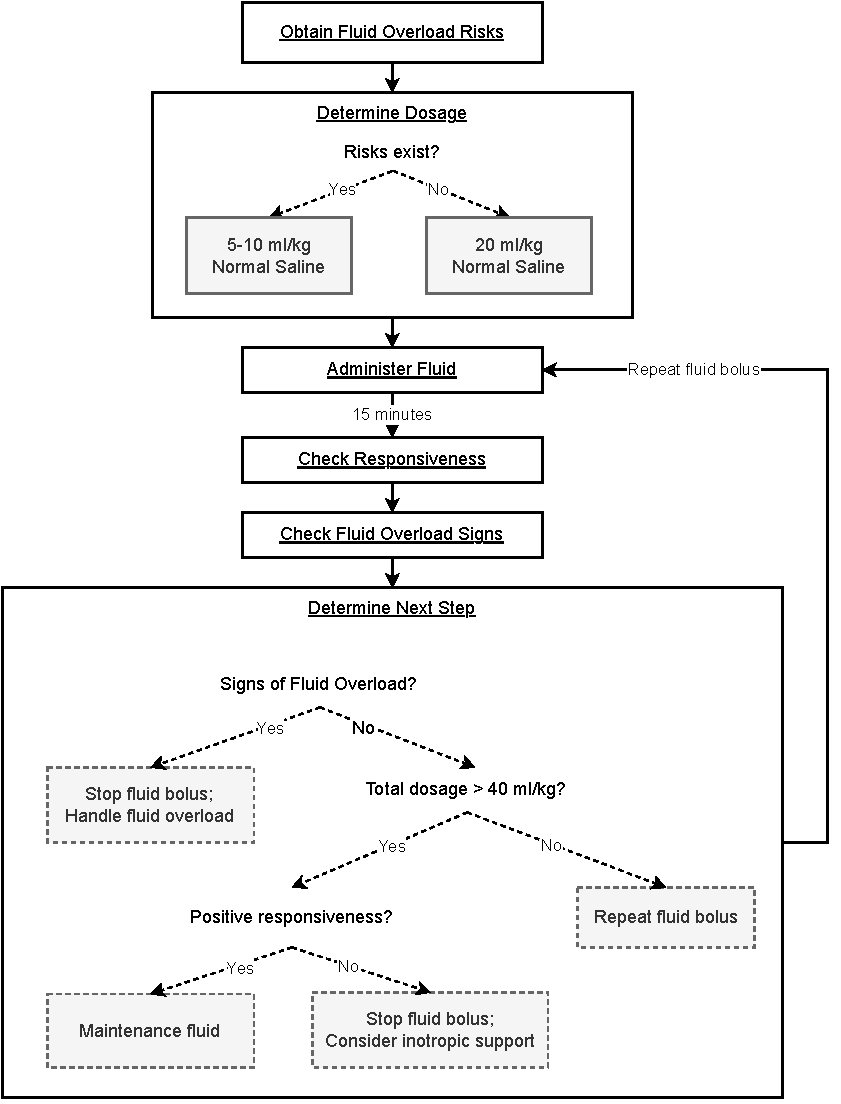
\includegraphics[scale=0.45]{FluidWorkflow-fmcad.pdf}
%  \caption{Fluid Resuscitation Guideline}\label{fig:fluid-therapy}
%\end{figure}
%
%This real-world \BPG{} exhibits characteristics common
%across many \BPGs{}. Specifically \BPGs{} typically:
%\begin{itemize}
%  \item Involve \stress{concurrent} workflows, such as administering drugs,
%    monitoring vitals, performing treatment, etc. There may also be
%    inter-workflow interactions. For instance, a diagnosis of sepsis during the
%    screening may require modifications to an ongoing course antibitiotics.
%  \item Often specified in a \stress{flowchart-like}
%    notation. See \cite{AHAFlowcharts} and \cite{CancerCareFlowcharts} for other flowchart-based \BPGs{} for management of \emph{cardiac arrest}, and
%    screening, risk-reduction, treatment and survivorship in
%    cancer care respectively.
%  \item Require communication between \stress{heterogeneous agents} such as
%     monitors and Electronic Health Records (EHRs).
%  \item Often use \stress{tables} indexed by parameters such as age, weight,
%    etc to present normal/abnormal ranges for measurements, or recommended dosages for drugs.
%\end{itemize}
%
%Note that the aforementioned characteristics are \emph{not} specific
%to one guideline. According to a review paper on \CIGs{} \cite{ClerqAIM03},
%such \DSLs{} should additionally
%\begin{enumerate*}[label=(\alph*)]
%  \item be formally defined, i.e, have a formal syntax and semantics, and
%  \item have an execution engine to provide decision support.
%\end{enumerate*}

In the following sections, we describe how these characteristics dictate the
design philosophy behind \MediK{}. We argue that this philosophy
makes \MediK{} both intuitive to \HCPs{}, and suitable for expressing
complex guidelines.

\section{\MediK{}}\label{sec:medik}

This section introduces the \MediK{} \DSL{} through its $\K$
syntax and semantics.
We developed $\MediK{}$ to realize
the semantics-first approach discussed in \autoref{sec:semantics-first}.
Thus, it has:
\begin{itemize}
  \item A formally defined, unambiguous semantics.
  \item A correct-by-construction interpreter derived from the semantics.
    As discussed in \autoref{chapter:evaluating-k},
  \item A comprehensive suite of formal program analysis tools.
  \item The ability to quickly adapt physician feedback, as only the semantics
    need to be changed an all tools evolve automatically.
\end{itemize}

The remainder of this section introduces the \MediK{} \DSL{}, and describes how it's
designed to accommodate characteristics of \BPGs{} discussed in
\autoref{sec:bpg-background}.

\subsection{\HCP{} Comprehensibility}

Our approach stresses that \HCPs{} must be able to comprehend the
guideline, and if necessary, making changes to on their own. As discussed
in \autoref{chapter:hurdles-cdss-adoption}, this has several hurdles, chief
among which is the fact that \HCPs{} are typically not trained to understand
conventionally programming languages. Thus, \HCPs{} need to work collaboratively
to translate the \BPG{} into a computable medium.
In essence, the \BPG{} serves as a functional
specification for implementing the \CDSS{}. But, this may lead to
a gap in the \HCPs{}' understanding of the system, and the actual
behavior.
To address this, we designed \MediK{}
s.t. encoded guidelines resemble their physical, non-executable counterparts,
with the intention that familiarity with non-executable guidelines
would also translate to computable \MediK{} ones.

Recall from \autoref{sec:generic-bpg} that \BPGs{}
typically involve concurrent workflows,
often expressed using a flowchart-like notation that may involve
inter-workflow interactions. In \autoref{sec:kacls-backend},
we discussed the merits and suitability of concurrently executing
state machines for modeling medical guidelines.
Thus, we looked at state-of-art languages for modeling large concurrent
systems using state machines, such as P \cite{DesaiPLDI13}, but made
adaptions to make expressing \BPGs{} easier.

In \MediK{}, like in P, programs are expressed as concurrently
executing instances of state machines that communicate via passing messages.
Given a \BPG{} where each workflow is expressed as a flowchart,
we express said flowcharts as State Machines in \MediK{}. Each flowchart node
in the \BPG{} is represented as a state in a state machine, and
edges are represented as state transitions. During execution,
instances of these machines are created, which interact with each other by
passing events. Note the distinction between
machine and its instance. A machine
is analogous to an Object Oriented Programming (OOP) class, whereas
its instance is analogous to an OOP object.

%We achieve this by defining \MediK{} (i.e., its syntax and semantics) in $\K$.
%$\K{}$ is a rewriting-based framework for defining executable
%semantics of languages, type systems and formal analysis tools.
%It has been successfully used to define executable semantics
%of many real world languages such as C \cite{HathhornPLDI15}, Java
%\cite{BogdanasPOPL15}, Javascript \cite{ParkPLDI15}, and the
%Ethereum Virtual Machine \cite{HildenbrandtCSF18}.
%We will introduce $\K$ by need while discussing \MediK{}. For more details on
%$\K$, we refer the reader to \cite{SerbanutaETNCS14} \cite{RosuJLAP10}.
%Once the executable
%semantics of a language have been defined in $\K{}$, it provides us with
%suite of tools such as an interpreter, deductive-verifier and a
%model-checker as shown in \figurename{} \ref{fig:k-overview}.

%The $\K{}$ ecosystem provides a suite of tools, such as an interpreter,
%model-checker, and deductive verifier that are parametric over the language's
%semantics, as shown in \figurename{} \ref{fig:k-overview}. Thus, by
%defining the semantics of \MediK{} in $\K{}$, we obtain aforementioned
%tools for it without any extra effort. Additionally:
%\begin{itemize}
%  \item The $\K$-based interpreter for \MediK{} essentially executes the language's
%    semantics rules, it is correct-by-construction.
%  \item Incorporating changes to \MediK{} only requires updating
%   the semantics. Since the tools are derived from the semantics,
%   they're automatically updated.
%\end{itemize}


%The remainder of this section introduces \MediK{} and describes
%how it's designed around characteristics of \BPGs{} from Section \ref{sec:motivating-example}.
%Recall that \BPGs{} typically involve concurrent workflows, often expressed using a
%flowchart-like notation that may involve
%inter-workflow interactions. To ensure \MediK{} programs are comprehensible
%to \HCPs{}, they must be representable in a flow-chart like notation that \HCPs{}
%are already comfortable with, and be capable of expressing inter-workflow
%interactions succinctly. To address these requirements, we borrow from
%from existing state-of-art languages for modeling large concurrent
%systems, like P \cite{DesaiPLDI13}, but make adaptions to make expressing and
%validating \BPGs{} easier. We explore the differences
%to existing techniques in section \ref{sec:related-works}.

Next, we describe \MediK{} using its $\K$-framework definition.
Recall from \autoref{sec:semantics-in-k}, the $\K{}$ definition
of a language has two components. The first is the language's
syntax, which is defined using a BNF-like notation. $\K{}$
utilizes this grammar to generate a parser for program in the language. We
describe \MediK{}'s syntax in depth in Section \ref{sec:syntax}.
The second is the semantics, which is defined using a $\K{}$-configuration and
rewrite rules. The $\K{}$-configuration
organizes the program's execution state. Rewrite rules
that operate over said configuration dictate the evolution
of program state during execution.
We describe the semantics in greater depth in Section
\ref{sec:semantics}\footnote{The complete executable semantics is available at
 \cite{medikUrl}.}

\subsection{Syntax}\label{sec:syntax}
We use the skeleton of a \MediK{} machine in \autoref{lst:machine-skeleton}, and use
it to describe the syntax.
Note that we use \inlinemedik{[...]} to denote
optional constructs, \inlinemedik{<...>} for mandatory constructs, lowercase for
terminals, and uppercase for non-terminals.
\begin{lstlisting}[
  float=ht,
  frame=single,
  style=mediksty,
  language=medik,
  numbers=left,
  numberstyle=\tiny,
  caption={Skeleton of a \MediK{} Machine},
  label={lst:machine-skeleton},
  xleftmargin=3ex
]
[init] machine <IDENTIFIER>                     @\label{lstline:machine-declaration}@
  receives <IDENTIFIER_LIST> {                  @\label{lstline:machine-receives}@
  vars <IDENTIFIER_LIST>;                       @\label{lstline:global-declarations}@

  [init] state <IDENTIFIER> {                   @\label{lstline:state-block-start}@
    entry [(IDENTIFIER_LIST)] {                 @\label{lstline:entry-block-start}@
      <STMT> // entry block
    }                                           @\label{lstline:entry-block-end}@
    on <IDENTIFIER> [(IDENTIFIER_LIST)] do {    @\label{lstline:handler-block-start}@
      <STMT> // event handler
    }                                           @\label{lstline:handler-block-end}@
  }                                             @\label{lstline:state-block-end}@
}
\end{lstlisting}
%A machine $m = \left(S, E, \Var, s_i\right)$,
%where $S$ is the set of states, $E$ the set of events,
%$\Var$, the set of instance variables, and $s_i$ the initial state.
%As shown in \figurename{} \ref{fig:machine-def}, a typical

A \MediK{} program consists of a set of machine definitions, where
a machine definition consists of:
\begin{itemize}
  \item (Lines \ref{lstline:machine-declaration}-\ref{lstline:machine-receives})
    The keyword \inlinemedik{machine}, followed by the name
    and a comma-separated list of identifiers signifying events that
    it \inlinemedik{receives} via the broadcast mechanism.
    One state in every machine, and one machine in a program can be
    prefixed with the keyword \inlinemedik{init}. On execution, an implicit instance
    of this machine the created, and the \inlinemedik{entry} block of
    initial state executed.
  \item (\autoref{lstline:global-declarations}) A set of instance variables.
  \item (Lines \ref{lstline:state-block-start}-\ref{lstline:state-block-end}) A set of state declarations. Each
    state has a name, an optional entry block (Lines
    \ref{lstline:entry-block-start}-\ref{lstline:entry-block-end}),
    and a set of event handlers (Lines \ref{lstline:handler-block-start}-\ref{lstline:handler-block-end}).
    The entry block begins with the keyword \inlinemedik{entry}, and may contain a list of variables
    that are bound to values when an instance enters the state during execution.
    One state in the machine may be prefixed with \inlinemedik{init}, specifying the
    initial state that an instance starts execution in.
  \item Event handlers begin with \inlinemedik{on} followed by the event name,
    an optional list of variables bound to data in the event, followed by the
    keyword \inlinemedik{do} a block of the handler's code.
\end{itemize}
%A machine definition starts with the keyword \inlinemedik{machine},
%followed by its name (\autoref{lstline:machine-declaration}). On
%\autoref{lstline:machine-receives}, following the
%\inlinemedik{receives} keyword, is a comma-separated list of identifiers
%signifying the events that the machine can receive from other machines.
%One machine in a program can be
%prefixed with the \inlinemedik{init} keyword. This machine is referred to as the
%initial machine.
%On \autoref{lstline:global-declarations}, following the keyword
%\inlinemedik{vars}, another comma-separeted list of identifiers signifies
%the instance-variables. During execution, each instance maintains a mapping from
%these variables to values. Each machine defines a set of states, such as
%the one in Lines \ref{lstline:state-block-start}-\ref{lstline:state-block-end}.
%A state has a name, an optional entry block
%(\autoref{lstline:entry-block-start}-\autoref{lstline:entry-block-end}),
%and a set of event handlers (Lines
%\ref{lstline:handle-block-start}-\ref{lstline:handler-block-end}). The entry block
%begins with the keyword \inlinemedik{entry}, and may contain a list of variables
%that are bound to values when the state is entered during execution.
%One state in the machine may be prefixed with \inlinemedik{init}, specifying the
%initial state. When execution begins, an implicit instance
%of the initial machine is created, and the \inlinemedik{entry} block of
%its initial state is executed. When an instance of a machine is dynamically
%created during runtime, the \inlinemedik{entry} block of its initial state is executed.
%Event handlers within a state begin with \inlinemedik{on} followed by the event name
%and an optional list of variables. When the event handler is executed, data from
%the received event's payload is bound to aforementioned variables which
%can be used in the code block that follows the \inlinemedik{do} keyword.
%A machine definition consists of:

%\begin{figure}[h]
%  \centering
%\begin{lstlisting}[style=mediksty,language=medik,basicstyle=\ttfamily\scriptsize,numbers=right]
%[init] machine <IDENTIFIER>
%  receives <IDENTIFIER_LIST> {
%  vars <IDENTIFIER_LIST>;
%
%  [init] state <IDENTIFIER> {
%    entry [(IDENTIFIER_LIST)] {
%      <STMT> // entry block
%    }
%    on <IDENTIFIER> [(IDENTIFIER_LIST)] do {
%      <STMT> // event handler code
%    }
%  }
%}
%\end{lstlisting}
%\caption{Machine Definition in \MediK{}}\label{fig:machine-def}
%\end{figure}

Each entry and event handler block contains statements defined
by syntax shown in \autoref{lst:medik-stmt-syntax}. The statements
are written over expressions given by the syntax in
\autoref{lst:medik-exp-syntax}.

Recall from \autoref{sec:semantics-in-k}, in $\K$, productions
are defined using the keyword \inlinek{syntax}, where
terminals are enclosed in quotes (\inlinek{""}), and non-terminals
begin with an upppercase character.

\MediK{} uses statement over expressions resemble counterparts in many commonly
used programming languages. For instance, Lines
\ref{lstline:value-start}-\ref{lstline:value-end} enable one to write
expressions using program identifiers (denoted by the builtin $\K{}$ production
\inlinek{Id}), and values such as booleans, or rationals, or \say{\inlinek{this}}, which enables
an instance to refer to itself. \autoref{lstline:dot-syntax} defines the usual dot operator (\inlinek{.}),
which can be used to access members of an instance.
Lines \ref{lstline:exp-syntax-begin}-\ref{lstline:exp-syntax-end} declare
common expressions such as \inlinek{+, -. >, >=} over rationals and \inlinek{&&, ||, !} over booleans.
We use the production \inlinek{StandaloneExp} to define certain expressions that
are typically not used in conjunction with other expressions, such as
\inlinek{new (...)} on \autoref{lstline:new-syntax} that resembles constructs in
OOP languages used to create object instances. Note however, that \MediK{} also
has several constructs not commonly found in other languages, such as
\inlinek{createFromInterface(...)} (\autoref{lstline:create-from-interface-syntax}) and \inlinek{obtainFrom(...)}
(\autoref{lstline:obtain-from-syntax}). We shall describe their need and purpose
in upcoming sections.

\begin{lstlisting}[
  float=ht,
  frame=single,
  style=ksty,
  basicstyle=\ttfamily\footnotesize,
  language=k,
  numbers=left,
  numberstyle=\tiny,
  xleftmargin=3ex,
  caption={\MediK{} Expressions Syntax},
  label={lst:medik-exp-syntax}
]
syntax StandaloneExp ::= "new" Id "(" Exps ")"                       [strict(2)] @\label{lstline:new-syntax}@
                       | "createFromInterface" "(" Id "," String ")" [strict(2)] @\label{create-from-interface-syntax}@
                       | Id "(" Exps ")"                             [strict(2)]
syntax Exp ::= Id                                                                @\label{lstline:value-start}@
             | Val
             | Rat
             | FloatLiteral
             | "this"                                                            @\label{lstline:value-end}@
             | UndefExp
             | "obtainFrom" "(" Exp "," Exp ")"            [seqstrict]           @\label{lstline:obtain-from-syntax}@
             | "(" Exp ")"                                 [bracket]
             > Exp "." Exp                                 [strict(1), left]     @\label{lstline:dot-syntax}@
             > Exp "+" Exp                                 [seqstrict, left]     @\label{lstline:exp-syntax-begin}@
             | Exp "-" Exp                                 [seqstrict, left]
             | Exp "*" Exp                                 [seqstrict, left]
             | Exp "/" Exp                                 [seqstrict, left]
             | Exp ">" Exp                                 [seqstrict, left]
             | Exp "<" Exp                                 [seqstrict, left]
             | Exp ">=" Exp                                [seqstrict, left]
             | Exp "<=" Exp                                [seqstrict, left]
             | "!" Exp                                     [seqstrict, left]
             | Exp "&&" Exp                                [strict(1), left]
             | Exp "||" Exp                                [strict(1), left]
             > Exp "==" Exp                                [seqstrict, left]     @\label{lstline:exp-syntax-end}@
             | "interval" "(" Exp "," Exp ")"
             > Exp "in" Exp
             | "parseInt" "(" Exp ")"                      [strict]
             | StandaloneExp
\end{lstlisting}

As reflected in \autoref{lst:medik-stmt-syntax} \MediK{} support many statements
commonly found in conventional programming languages, such as
variable assignment (\autoref{lstline:assignment-stmt}), \inlinemedik{if-else}
(Lines \ref{lstline:if-stmt} and \ref{lstline:if-else-stmt}) and \inlinemedik{while}
(\autoref{lstline:while-stmt}). Others, such as \inlinemedik{broadcast} (Lines
\ref{lstline:broadcast-stmt-macro} and \ref{lstline:broadcast-stmt-syntax}),
\inlinemedik{goto} and \inlinek{interface} declarations have nuanced meanings,
and will be explained in upcoming sections.

\begin{lstlisting}[
  float=h
  ,style=ksty
  ,language=k
  ,basicstyle=\ttfamily\footnotesize,
  ,numbers=left
  ,numberstyle=\tiny
  ,xleftmargin=3ex
  ,caption={\MediK{} Statement Syntax}
  ,label={lst:medik-stmt-syntax}
]
  syntax Stmt ::= StandaloneExp ";"                               [strict]
                | "sleep" "(" Exp ")" ";"                         [strict(1)]
                | "send" Exp "," ExtId ";"                        [macro]
                | "send" Exp "," ExtId "," "(" Exps ")" ";"       [seqstrict(1, 3)]
                | "broadcast" Id ";"                              [macro]     @\label{lstline:broadcast-stmt-macro}@
                | "broadcast" Id "," "(" Exps ")" ";"             [strict(2)] @\label{lstline:broadcast-stmt-syntax}@
                | "goto" Id ";"                                   [macro]
                | "goto" Id "(" Exps ")" ";"                      [strict(2)]
                | "print" "(" Exp ")" ";"                         [strict]
                > "return" ";"                                    [macro]
                | "return" Exp ";"                                [strict(1)]
                | "var" Id "=" Exp ";"                            [macro]
                > Exp "=" Exp ";"                                 [strict(2)] @\label{lstline:assignment-stmt}@
                > "var" Id ";"
                | "vars" Ids ";"                                  [macro-rec]
                | Block
                > "if" "(" Exp ")" Block                          [strict(1)] @\label{lstline:if-stmt}@
                | "if" "(" Exp ")" Block "else" Block             [strict(1)] @\label{lstline:if-else-stmt}@
                | "while" "(" Exp ")" Block                                   @\label{lstline:while-stmt}@
                | "entry" Block                                   [macro]
                | "entry" "(" Ids ")" Block
                | "on" ExtId "do" Block                           [macro]
                | "on" ExtId "(" Ids ")" "do" Block
                | "fun" Id "(" Ids ")" Block
                | NonDetStmt
                | Exp "in" "{" CaseDecl "}"
                | StateDecl
                > "machine" Id Block                              [macro]
                | "machine" Id "receives" Ids Block
                | "interface" Id Block                            [macro]    @\label{lstline:interface-declaration}@
                | "interface" Id "receives" Ids Block                        @\label{lstline:interface-declaration}@
                | "init" "machine" Id Block                       [macro]
                | "init" "machine" Id "receives" Ids Block
                | "yield" ";"
                > Stmt Stmt                                       [right]
\end{lstlisting}

In lines 7-15, we define syntax for \MediK{} statements. Some of these,
such as variable assignment (line 7), \inlinek{if-else} (line 8)
and \inlinek{new Id(..);} (line 9) are commonly found in other languages, and
have expected meanings. The remaining statements (lines 10-15) have nuanced
meanings in context of state machines. We shall go over these while discussing
\MediK{}'s semantics in section \ref{sec:semantics}.

%\begin{figure}[b]
%  \centering
%\begin{lstlisting}[style=ksty,language=k,basicstyle=\ttfamily\scriptsize,numbers=right]
%configuration
%  <instance multiplicity="*" type="Map"> ...
%    <k> createMachineDefs($PGM)
%     ~> createInitInstances </k>
%    <genv> .Map </genv>
%    <env> .Map </env>
%    <inBuffer> .List </inBuffer>
%    <activeState> . </activeState>
%  </instance>
%  <machine multiplicity="*" type="Map"> ...
%    <machineName> . </machineName>
%    <states>
%      <state multiplicity="*" type="Map">
%        <stateName> . </stateName>
%        <entryBlock> . </entryBlock>
%        <eventHandlers> ... </eventHandlers>
%      </state>
%    </states>
%  </machine>
%\end{lstlisting}
%\caption{\MediK{}'s $\K$ Configuration}\label{fig:k-config}
%\end{figure}

\subsection{Semantics}\label{sec:semantics}
% Once the syntax has been defined, $\K$ can
% automatically generate a parser for programs in the language.
% The semantics, described via $\K$ rewrite rules, describe
% how the program evolves
% during execution.
Semantics of a language defined in $\K$ has two components:
\begin{enumerate*}[label=(\arabic*)]
  \item description of program state via $\K$-configurations, and
  \item $\K$ rules that dictate state evolution.
\end{enumerate*}
Next we describe these components in detail.

\subsubsection{$\K{}$-Configuration}
$\K$ represents program execution state using $\K$-configurations.
A $\K$-configuration is an unordered list of (potentially nested) \emph{cells},
specified using an XML-like notation.
When declaring rules (as rewrites) over this state,
any subset of the cells present in the configuration can be mentioned.
This allows specifying only necessary parts of the state for a given rule,
letting $\K{}$ assume that the rest of the configuration remains unchanged.
The following configuration defines the initial state for any \MediK{} program:

\begin{lstlisting}[
  style=ksty
  ,language=k
  ,basicstyle=\ttfamily\scriptsize
  ,numbers=left
  ,numberstyle=\tiny
  ,framexleftmargin=1.5em
  ,xleftmargin=2em
  ]
configuration
  <instance multiplicity="*" type="Map"> ...
    <k> createMachineDefs($PGM)
     ~> createInitInstances </k>
    <genv> .Map </genv>
    <env> .Map </env>
    <inBuffer> .List </inBuffer>
    <activeState> . </activeState>
  </instance>
  <machine multiplicity="*" type="Map"> ...
    <machineName> . </machineName>
    <states>
      <state multiplicity="*" type="Map">
        <stateName> . </stateName>
        <entryBlock> . </entryBlock>
        <eventHandlers> ... </eventHandlers>
      </state>
    </states>
  </machine>
\end{lstlisting}

The keyword \inlinek{configuration} (line 1) defines a $\K{}$-configuration,
followed by xml-like notation for the $\K$-cells. For example \inlinek{<foo> ... </foo>}
corresponds to a $\K$-cell with the name \inlinek{foo}.
The \inlinek{<instance>} cell (lines 2-9) contains state of each \MediK{}
machine instance during execution. Each instance manages its
instance variables using a map in the \inlinek{<genv>} cell (line 5),
a buffer of incoming events in the \inlinek{<inBuffer>} cell (line 7)
and the currently executing code in the \inlinek{<k>} cell (lines 3-4).\footnote{For brevity, we present a simplified version of the configuration. See \cite{medikUrl} for the entire configuration.}
When a \MediK{} program is executed, $\K$ replaces \inlinek{$PGM} (line 3) with the Abstract Syntax Tree (AST)
of the program, obtained by parsing the program using the syntax from
section \ref{sec:syntax}.
The \inlinek{createMachineDefs} constructs
is defined (using rewrite rules) to traverse the program AST
and populate the configuration with information related to each machine.
The \inlinek{createInitInstances} creates an instance for the machine
with the \inlinek{init} keyword, leading to execution of the initial
machine's entry block. Note that \scantokens{\lstinline{~>}} symbol (line 3)
is interpreted by $\K$ as \say{followed-by}, i.e., execution of \inlinek{createMachineDefs}
is followed by execution of \inlinek{createInitInstances}.
The attribute \inlinek{multiplicity="*"}
on lines 2 and 10 signifies that multiple copies of the
corresponding cells, in this case \inlinek{<machine>} and \inlinek{<instance>} cells,
can exist in the configuration during execution. This allows, during execution,
for multiple machine definitions, each with multiple
instances, to exist.
The \inlinek{<machine>} cell (lines 10-19) holds information relevant to
a machine definition, such as the name in the \inlinek{<machineName>}
cell (line 11) and states in the \inlinek{<states>} cell (lines 12-18).
The \inlinek{<state>} (lines 13-17) holds information
relevant to a state, such as the entry block in cell
\inlinek{<entryBlock>} (line 15) and event handlers in cell
\inlinek{<eventHandlers>} (line 16).
%using the \inlinek{createMachineDefs}
%construct, and new instances for those definitions, using the \inlinek{new} keyword.


\subsubsection{$\K$-Rules}
$\K$-rules operate over the configuration and
define the evolution of program state during execution. A $\K$-rule
begins with the keyword \inlinek{rule}, and is a statement of the form $\phi
\Rightarrow \psi$, where $\phi$ and $\psi$ are
patterns over configuration terms and $\K$-variables. We
say $\phi$ is the $\LHS$ and $\psi$ is the $\RHS$ of the rule.
Let substitution $\theta$ be a map from $\K$-variables to terms. Say, for given
pattern $\phi$ and substitution $\theta$, $\phi\theta$ be the term
obtained by replacing each variable $v$ in $\phi$ with $\theta(v)$.
During execution, if the current configuration $C$, i.e. program execution state,
matches $\phi$ with substitution $\theta$, then it is rewritten to
$\psi\theta$. We say pattern $\phi$ matches configuration $C$ iff
there exists a substition $\theta$ s.t. $C = \phi\theta$.
For example, consider the following rule for updating the value of a local program variable.
\begin{lstlisting}[
  style=ksty
  ,language=k
  ,basicstyle=\ttfamily\scriptsize
  ,numbers=left
  ,numberstyle=\tiny
  ,framexleftmargin=1.5em
  ,xleftmargin=2em
  ]
rule <k> I:Id = V:Val => V ... </k>
     <env> (I |-> Loc) ... </env>
     <store> Store => Store[Loc <- V] </store>
\end{lstlisting}
Here, \inlinek{I}, \inlinek{V}, \inlinek{Loc}, and \inlinek{Store}
are $\K$-variables. Note the distinction between program variables and $\K$-variables:
while program variables are simply identifiers, $\K$-variables have logical meaning.
The \inlinek{...} is used to denote parts of the configuration
not relevant to the rule.
Typically, the top of the \inlinek{k} cell contains the statement currently
being executed. Suppose we're executing the statment \inlinek{i = 2;}. In this
case, the current configuration will have a \inlinek{k} cell of the form
\inlinek{<k> i = 2 ... </k>}, an environment cell \inlinek{env} where variable
\inlinek{i} maps to some pointer $p$, and a store cell
\inlinek{store} containing a map $M$ with some value pointed-to by $p$.
The $\LHS$ matches with substitution
$\theta = \left(I \mapsto i, V \mapsto 2, Loc \mapsto p, Store \mapsto M\right)$,
resulting in the top of the \inlinek{k} cell to be rewritten to the value $2$,
and pointer $p$ updated to point to $2$ in $M$.
Note if there exist multiple rules that can match the current configuration,
then one rule is non-deterministically chosen and applied. An execution is a
sequence of rule applications that continues until no rule matches the configuration.

The following sections we present several \MediK{} constructs relevant to
defining \BPGs{} using their $\K$-rules. We first present the
rule for sending and receiving messages.
\begin{lstlisting}[
  style=ksty
  ,language=k
  ,basicstyle=\ttfamily\scriptsize
  ,numbers=left
  ,numberstyle=\tiny
  ,framexleftmargin=1.5em
  ,xleftmargin=2em
  ]
rule
<instance>
 <k> send instance(RecvId) , EventName:Id , ( Args )
     =>  done ... </k> ...
</instance>
<instance>
 <id> RecvId </id> ....
 <inBuffer> ... (.List
  => ListItem(
      eventArgsPair(EventName | Args | Epoch + 1
      )))
 </inBuffer> ...
</instance>
<epoch> Epoch </epoch>
\end{lstlisting}
When the top of the \inlinek{k} cell has
\inlinek{send},  the rule above
\begin{enumerate*}[label=(\roman*)]
  \item obtains the \inlinek{id} of the receiver instance,
    the event name and the event arguments by matching
    the variables \inlinek{RecvId}, \inlinek{EventName} and \inlinek{Args}
    against the current configuration (line 3),
  \item rewrites the top of the \inlinek{k} cell (line 4) to \inlinek{done},
    marking the completion of execution for the construct,
  \item adds the event and associated arguments to the
    buffer of incoming events (lines 8-12) of the instance
    with \inlinek{id} \inlinek{RecvId} (line 7).
  \item The \epoch{} decides when the machine can run, and is discussed in
    Section \ref{sec:scheduling-semantics}.
\end{enumerate*}

To handle interaction with heterogeneous external sources, \MediK{}
models them as interfaces. An interface is a \FSM{} that has its
transition system defined externally. For example, certain measurements
such as the heart rate are often obtained from sensors.
The following code shows the process of obtaining external measurements in
\MediK{}.
\begin{lstlisting}[
  style=mediksty
  ,language=medik
  ,basicstyle=\ttfamily\scriptsize
  ,numbers=left
  ,numberstyle=\tiny
  ,framexleftmargin=1.5em
  ,xleftmargin=2em
  ]
interface HeartRateSensor { }

machine TreatmentMachine { ...
  var hrSensor = createFromInterface(HeartRateSensor,
                              "heartRateSensor");
  var heartRate = obtainFrom(hrSensor, "heartRate");
}
\end{lstlisting}
Since we don't have the transition system for
the heart rate sensor, we declare it as an interface (line 1).
Next, instead of using \inlinemedik{new} to create an instance, we use
a builtin \MediK{} construct \inlinemedik{createFromInterface}, which takes as
arguments
\begin{enumerate*}[label=(\alph*)]
  \item the inteface name (lines 4),
  \item a unique identifier string used to identify the
    instance outside the \MediK{} process.
\end{enumerate*}
All other \MediK{} machines can interact with external sensor using
variable \inlinemedik{hrSensor}. There is no need to make any distinction
between external, and \MediK{}-based machines.
To deal with external interactions, input and output
pipes are provided to the \MediK{} process at launch.
When the \inlinemedik{send} construct is used on an external machine,
\MediK{} will write
a JSON \cite{jsonUrl} message with the event data, the
identifier from line 5, and a unique transaction id
to the \emph{write-end} of the output pipe. At the
\emph{read-end}, we need to write external code (in any programming language)
to handle the JSON message. In the example above, this involves reading from
the external heart rate sensor. To send data to \MediK{}, a JSON message in
a pre-specified format needs to be written to the \emph{write-end} of the
input pipe.

Next, we desribe the rule for supporting tables in \MediK{}.
Once a measurement, such as the heart rate has been obtained
from a sensor, we need to use a table, such as \tablename{} \ref{table:vital-signs}
to check if the measurement is within a normal range. In \MediK, we can write a
function that does the required check, as shown in \figurename{}
\ref{fig:hr-check-fun}.
\begin{figure}[h]
  \centering
\begin{lstlisting}[
  style=mediksty
  ,language=medik
  ,basicstyle=\ttfamily\scriptsize
  ,numbers=left
  ,numberstyle=\tiny
  ,framexleftmargin=1.5em
  ,xleftmargin=2em
  ]
fun isHeartRateNormal() {
  days(age) in {
    interval(days(0)  , months(1)): return hr > 205;
    interval(months(1), months(3)): return hr > 205;
    // omitting other cases
    default                       : return hr > 100;
  }
}
\end{lstlisting}
  \caption{Checking abnormality using tables}\label{fig:hr-check-fun}
\end{figure}
In the code, if the \inlinemedik{age} lies in
any of the intervals (closed on the left, open on the right) on lines 3-5, the
corresponding statement to the right of the colon (\inlinemedik{:}) is run. Otherwise
line 6 is run.
In \MediK{}, the following rules are responsible for assigning semantics to
the \inlinemedik{in-interval} construct:
\begin{lstlisting}[
  style=ksty
  ,language=k
  ,basicstyle=\ttfamily\scriptsize
  ,numbers=left
  ,numberstyle=\tiny
  ,framexleftmargin=1.5em
  ,xleftmargin=2em
  ]
rule E in interval(L, U) => (E >= L) && (E < U)
  [macro]
rule E in { interval(L, U): S:Stmt Cs:CaseDecl }
  => if (E in interval(L, U)) {S} else {E in { Cs }}
  [macro-rec]
\end{lstlisting}

Note the rules above are marked with the attributes \inlinek{macro}
(line 2) or \inlinek{macro-rec} (line 5). This specifies that
these constructs are not part of the language's semantics, but merely
syntactic sugar. On line 1, we specify that
\inlinek{E in interval(L, R)} desugars to checking the expression \inlinek{e}
is between the lower and upper bound \inlinek{L} and \inlinek{U} respectively.
Similary we desugar each case statement to an \inlinek{if-else} statement.
In lines 3-5, we say that if the expression \inlinek{E} is in
\inlinek{interval} with lower and upper bounds \inlinek{L} and \inlinek{U}
respectively, then execute \inlinek{S}, otherwise check \inlinek{E} against the
remaining cases \inlinek{Cs}. Note the postfix \inlinek{-rec} after
\inlinek{macro} specifies that the rule applies recursively, to desugar
the remaining case statements.

\paragraph{\MediK{} Scheduling Semantics}\label{sec:scheduling-semantics}

Since the $\K{}$-generated
interpreter is single-threaded, \MediK{} employs interleaving-semantics
for concurrency, using a single \inlinemedik{executor} thread shared
between machine instances. A machine instance that is either at the start of
an entry block, or has an event in the input buffer that it can handle is
said to be \emph{enabled}, i.e. one that can run once the \inlinemedik{executor}
becomes available. But, a naive strategy that non-deterministically
chooses one \emph{enabled} machine instance may lead to unfairness.
Specifically, there may be situations where a machine instance is
\emph{enabled} but is never chosen for execution.
Therefore, to ensure fairness, we use a scheduling strategy based on a monotonically
increasing global counter called the \epoch{}.
% Instead of just tracking
% \emph{enabled} machines, we also track the \epoch{} value at which
% said machines became enabled.
We show this execution strategy in \figurename{}
\ref{fig:scheduling-semantics}

\begin{figure}[ht]
  \centering
    \begin{algorithmic}[1]

    \State $\epoch{} \gets 0$
      \State $\scheduled{} \gets \left\{ \Instance_{\Machine{}_{0},0}^{0} \right\}$
    \While{$\scheduled{} \neq \emptyset$}
       \State \begin{varwidth}[t]{\linewidth}
           $\Instance_{\Machine_{i},j}^{\tau} \gets \textit{choose}\left(\scheduled{}\right) \text{ s.t. }$
           \par
              \hskip\algorithmicindent $\qquad \tau \leq \epoch{} \wedge \enabled(\Instance_{\Machine_{i},j}^{\tau})$ \par
            \end{varwidth}
      \State $\scheduled{} \gets \scheduled \setminus \Instance_{\Machine_{i},j}^{\tau}$
      \State $\textit{execute}(\Instance_{\Machine_{i},j}^{\tau}, \scheduled{})$
      \If{$\not\exists i',j',\tau'$ s.t.
      $(\Instance_{\Machine_{i'},j'}^{\tau'} \in \scheduled{})$
      \\ \qquad \qquad $\wedge (\tau' \leq \epoch{}) \wedge (\enabled(\Instance_{\Machine_{i'},j'}^{\tau'}))$}
      \newline
       \State $\epoch{} \gets \epoch{} + 1$
      \EndIf
    \EndWhile
  \end{algorithmic}
  \caption{\MediK{} Scheduling Semantics}\label{fig:scheduling-semantics}
\end{figure}

Recall from Section \ref{sec:syntax} that a \MediK{} program consists of a set
of machines, of which one, prefixed with the keyword \inlinemedik{init}, is the \emph{initial} machine.
Each machine has one state prefixed with \inlinemedik{init}, referred to as the
\emph{initial} state.
Let $P = \{ \Machine_{0}, \Machine_{1}, \dots, \Machine_{n-1} \}$ be a program
with $n$ machines, where $\Machine_{0}$ is prefixed with \inlinemedik{init}.
\MediK{} allows instances of a machine to be created dynamically at runtime.
For machine $\Machine_i \in P$, let $\Instance_{\Machine_i,j-1}$ be its
$j$-th instance.

Execution begins in \epoch{} zero with the implicit (first) instance of the
initial machine, denoted by $\Instance_{\Machine_{0},0}^{0}$.
We use $\Instance_{\Machine_{i},j-1}^{\tau}$ to
say that the $j$-th instance of machine $\Machine_{i}$
is scheduled for execution in \epoch{} $\tau$.
Recall that a state definition may have an entry block, containing code
that is executed when the state is entered, or event handlers containing
code that is executed when an event is dequeued from the input buffer. When execution
begins, the entry block of the \emph{initial state} of the \emph{implicit instance}
of the \emph{initial machine} $\Instance_{\Machine_0,0}$ becomes scheduled (line 2) at \epoch{} 0.
On line 4, an instance $\Instance_{\Machine_{i},j}^{\tau}$ is
non-deterministically chosen from all machines that are both scheduled to run when
$\tau \leq \epoch{}$ and \textit{enabled}. We use
$\textit{execute}(\Instance_{\Machine_{i},j}^{\tau}, \scheduled{})$ on line 5
to denote this execution process. Execution of the entry or event handler block is atomic,
i.e., a context-switch can only occur at the end of the block. Note that when
a new instance of a machine is created using the keyword \inlinemedik{new}, the
\emph{entry} block of the \emph{initial} state of the \emph{target} machine
is executed synchronously before control returns to the source machine, and the
instance is added to the multiset of \textit{scheduled} machines.
A context switch only occurs in three cases: \inlinemedik{goto}, \inlinemedik{sleep}, and \inlinemedik{obtainFrom},
which we describe later.

During execution, if an instance $\Instance_{\Machine_i,j}$ sends an event
to another instance $\Instance_{\Machine_{i'},j'}$, then
the event is scheduled to be handled by $\Instance_{\Machine_{i'},j'}$ in or
after the next epoch, i.e., $\scheduled{} \gets \scheduled{} \cup
\{\Instance_{\Machine_{i'}, j'}^{\epoch{}+1}\}$. Similary, if a \inlinemedik{goto}
statement is encoutered, the entry block of the target state is scheduled
for execution at \epoch{} + 1. If no other machine is both \textit{scheduled} to run
in the current \epoch{}, and \textit{enabled}, then the \epoch{} advances by one (line 8).

%\MediK{} employs a simple epoch-based scheduling approach.
%Execution begins in epoch 0, with
%
%
%\begin{lstlisting}[style=mediksty,language=medik,basicstyle=\ttfamily\scriptsize,numbers=left]
%rule
%<k>   enterState(SName | Args | Scheduled )
% =>   StateDecls
%   ~> assign(BlockVars | Args)
%   ~> EntryBlock
%   ~> releaseExecutor
%   ~> handleEvents ...
%</k>
%<activeState> _ => SName </activeState>
%<env> _ => .Map </env>
%<class> MName </class>
%<machine>
% <machineName> MName </machineName>
%  <state>
%   <stateName> SName </stateName>
%   <stateDeclarations>
%    StateDecls
%   </stateDeclarations>
%   <entryBlock> EntryBlock </entryBlock>
%   <args> BlockVars </args> ...
%  </state> ...
% </machine>
%<executorAvailable>
%  true => false
%</executorAvailable>
%<epoch> Current </epoch>
% requires Scheduled <=Int Current
%\end{lstlisting}

%Initially, the machine prefixed with the \inlinemedik{init} is
%executed, at epoch 0. We say a machine is enabled, if:
%\begin{enumerate*}[label=(\roman)]
%  \item it is at the start of an entry block of a state,
%  \item the entry block
%\end{enumerate*}


\paragraph{Timer Semantics}
Next, we discuss how \MediK{} handles temporal aspects of \BPGs{}. For instance, consider the
Fluid resuscitation guideline \BPG{} from Section \ref{fig:fluid-therapy}.
After administering fluids, the \BPG{} recommends waiting for 15 minutes
before evaluating their effectiveness. This waiting behavior in
\MediK{} is implemented using a \inlinemedik{sleep(duration)} statement.
Formalizing the execution semantics of such a statement in $\K{}$ presents
a challenge as $\K{}$ does not provide builtin support for timers. Therefore,
in \MediK{}, \inlinemedik{sleep(duration)} is described by the following rule:
\begin{lstlisting}[
  style=ksty
  ,language=k
  ,basicstyle=\ttfamily\scriptsize
  ,numbers=left
  ,numberstyle=\tiny
  ,framexleftmargin=1.5em
  ,xleftmargin=2em
  ]
rule <k> sleep(Duration:Int) ;
      =>    jsonWrite( { "action"   : "sleep"
                       , "duration" : Duration
                       , "tid"      : TId }
                       , ... )
         ~> releaseExecutor
         ~> waitForSleepResponse(TId) ...
     </k>
     <tidCount> TId => TId +Int 1 </tidCount>
\end{lstlisting}
\inlinemedik{sleep} results in a JSON message being sent to a remote
endpoint (lines 1-5) specified when the \MediK{} process is launched. This mimics
sending an event to an external \emph{timer} machine, with the desired duration
as the payload. At the remote endpoint,
code must be provided (in any programming language) to parse the message, and
respond with a JSON message indicating the expiration of the timer
once the desired duration has passed. A unique transaction-id (lines 4, 7, 9),
which the code at the endpoint is expected to provide in the response,
uniquely identifies the machine instance being responded to.
\inlinemedik{sleep} causes a context-switch to occur on line 6, releasing the
executor lock to process other \emph{scheduled} machines.

When a message signifying the expiration of the timer is sent to
the \MediK{} process, along with the transaction id of source instance,
the corresponding event signalling the completion of the sleep statement
is placed at the \emph{beginning} of the source machine instance's input buffer,
and the instance is scheduled to resume execution in the next epoch.
The following rule handles the external response:
\begin{lstlisting}[
  style=ksty
  ,language=k
  ,basicstyle=\ttfamily\scriptsize
  ,numbers=left
  ,numberstyle=\tiny
  ,framexleftmargin=1.5em
  ,xleftmargin=2em
  ]
rule
<k> waitForSleepResponse(TId) => . ... </k>
<inBuffer>
  (ListItem(event($SleepDone | TId | Tau ))
 => .List)  ...
</inBuffer>
<executorAvailable>
  true => false
</executorAvailable>
<epoch> Epoch </epoch>
  requires Tau <=Int Epoch
\end{lstlisting}
The \inlinemedik{waitForSleepResponse(TId)}
blocks execution until the external response indicating
the expiration of the sleep timer is received in the input buffer (line 4).
Once the response is received, the machine instance resumes execution when
\begin{enumerate*}[label=(\alph*)]
  \item the execution lock becomes available
  (indicated by \inlinemedik{true} on line 8), and,
  \item the epoch the instance was scheduled in (line 4) is less than or equal to the current
  epoch (lines 10-11).
\end{enumerate*}

An \inlinemedik{obtainFrom} statement also results in a context switch.
Just as in the case of sleep, a json message is sent to the remote
endpoint, while the machine instance release the execution lock, and waits for a
response. Once data for the requested field is available, it's communicated as an
event to the \MediK{} process, and the machine resumes execution.
%
%\begin{lstlisting}[style=ksty,language=k,basicstyle=\ttfamily\scriptsize,numbers=right]
%rule
%<k> obtainFrom(instance(Id:Int), Field:String)
%    =>   jsonWrite( { "name"      : "Obtain"
%                    , "args"      : [ Field , .JSONs ] } ...)
%      ~> releaseExecutor
%      ~> waitForObtainResponse(TId) ...
%   </k>
%   <tidCount> TId => TId +Int 1 </tidCount>
%\end{lstlisting}


\section{Evaluation}\label{sec:evaluation}

\subsection{Sepsis Management \CDSS}

To evaluate our approach, we collaborated with the Children's Hospital
of Illinois at OSF St. Francis Medical Center to develop a \MediK{}-based
\CDSS{}
for screening and management of Pediatric Sepsis \footnote{the entire \CDSS{}
for sepsis management is available at \cite{psepsis-url}.}.

Recall from \figurename{} \ref{fig:sepsis-screening} the guideline
for sepsis screening.
In \figurename{} \ref{fig:medik-sepsis-screening}, we show
\MediK{} code corresponding to the sepsis screening guideline.
When modeled in \MediK{}, a flowchart in the guideline is represented using
a \MediK{} machine. \emph{Nodes} in the flowchart are represented as
\emph{states} in a \MediK{} machine, while flowchart \emph{edges} as \emph{state-transitions}.
Note that we use \emph{node} to refer to constructs
in the flowchart, and \emph{state} to refer to counterparts in \MediK{}.
Also, while it's desirable to represent each flowchart \emph{node} as a
state machine \emph{state}, the task in the flowchart \emph{node} may warrant using
multiple state-machine \emph{states}. For example,
in \figurename{} \ref{fig:sepsis-screening}, the step \say{Obtain Patient Age,
Weight, and High Risk Conditions} is translated to states \inlinemedik{ObtainAge} (lines
7-13), \inlinemedik{ObtainWeight} (line 14), and
\inlinemedik{ObtainHighRiskConditions} (line 15) in \figurename{} \ref{fig:medik-sepsis-screening}.
Within each of these states, the code
permits communication with heterogeneous external agents for obtaining
required parameters. For instance, on line 9, an
\inlinemedik{Instruct} event is sent to an external \inlinemedik{tablet} machine
with the payload \inlinemedik{"get age"}. The recipient process
runs on a tablet held by the Healthcare Provider, and handles
the event by prompting the provider to enter the patient's age.
A \inlinemedik{ConfirmAgeEntered} event, emitted once the age
is obtained, enables the screening machine to proceed to the next
step (lines 11-13). Once all appropriate measurements have been obtained,
they are checked for abnormality (lines 18-26) using tables shown in \figurename{}
\ref{fig:hr-check-fun} to arrive upon a diagnosis.

\begin{figure}
  \centering
\begin{lstlisting}[style=mediksty
,language=medik
,basicstyle=\ttfamily\scriptsize
,numbers=left
,numberstyle=\tiny
,framexleftmargin=1.5em
,xleftmargin=2em
]
machine SepsisScreening receives .. {
  init state Start {
    on StartScreening do {
      goto ObtainAge;
    }
  }
  state ObtainAge {
    entry {
      send tablet, Instruct, ("get age");
    } on ConfirmAgeEntered do {
      goto ObtainWeight;
    }
  }
  state ObtainWeight { ... }
  state ObtainHighRiskConditions { ... }
  state CalculateScore {
      var hrAbnormal = !isInNormalRange("HR", ...);
      var bucket1    = hrAbnormal ||  ...
      var bucket3    = mentalStatusAbnormal || ...

      var sepsisSuspected
        = bucket1 && bucket2 && bucket3;

      send tablet, SepsisDiagnosis
        , (sepsisSuspected);
  }
}
\end{lstlisting}
  \caption{Sepsis Screening in \MediK{}}\label{fig:medik-sepsis-screening}
\end{figure}

%Apart from structurally resembling the workflow, the code
%permits communication with heterogenous external agents, and
%\emph{obtains} patient parameters such as age and weight, and
%uses them to evaluate the patient for sepsis. For instance on line 9,
%we send an event to the external machine that is the tablet held by the \HCP{},
%to obtain the patient's age. Once the age is entered, an event
%\inlinemedik{ConfirmAgeEntered} is sent to the machine, prompting the machine to
%move on to collecting the patient's weight.
% When evaluating whether the patient
%meets the criteria for sepsis, we use functions, such as the one on line 18,
%that obtain the value from a sensor, and check whether
%it lies in acceptable ranges using tables
%indexed by the patient's age and weight, similar to the paper-based \BPG{}.
%Treatment machines \emph{receive} events from
%the screening machine, and are triggered if the diagnosis is \textit{sepsis
%positive}, suggesting commencement of treatment.

\begin{figure}[b!]
  \centering
\begin{lstlisting}[style=mediksty
,language=medik
,basicstyle=\ttfamily\scriptsize
,numbers=left
,numberstyle=\tiny
,framexleftmargin=1.5em
,xleftmargin=2em
]
machine FluidTherapy
  receives StartFluidTherapy, ... {


  init state Start {
    on StartFluidTherapy do {
      goto ObtainRisks;
    }
  }

  state ObtainRisks {
    // Obtain fluid overload related risks
  }

  state SuggestFluidDosage {
    // Suggest a dosage based on risks
  }

  state WaitForAdministerFluidConfirmation {
    // Handler for Normal Saline Administration
    on ConfirmNormalSalineAdministered do {
      sleep(900);
      goto EvaluateResponsiveness;
    }
  }

  state EvaluateResponsiveness {
    entry {
      send tablet
        , Instruct
        , ("get responsiveness to fluids");
    }

    on FluidResponsivenessEntered(responsiveness) do {
      isResponsiveToFluids = responsiveness;
      goto ObtainFluidOverloadSigns;
    }
  }
  state ObtainFluidOverloadSigns {
    // Obtain signs of fluid overload
  }

  state AskNextStep {
    entry {
      var recommendation;
      if (this.fluidOverload) {
        recommendation = "handle fluid overload";
      } else {
        // obtain total saline dose
        if ((totalSalineDose >
              measurementBounds.salineDosageUpperBound) {
          if (isResponseiveToFluids) {
            recommendation = "maintainence fluids"
          } else {
            recommendation = "consider inotropic support";
            broadcast ConsiderInotropicSupport;
          }
        } else {
          recommendation = "repeat fluid bolus";
        }
      }
      // Send recommendation to tablet
      // Wait for HCP response
    }
  }
}
\end{lstlisting}
  \caption{Fluid Resuscitation in \MediK{}}\label{fig:medik-fluid-therapy}
\end{figure}


Recall from Section \ref{sec:motivating-example} that once a sepsis diagnosis has been arrived upon,
one of the guideline suggested actions include administering fluids as shown in
\figurename{} \ref{fig:fluid-therapy}. In \figurename{} \ref{fig:medik-fluid-therapy},
we show the corresponding \MediK{} code for administering fluids.
The process starts when an external \inlinemedik{StartFluidTherapy} event,
corresponding to a button press by the \HCP{} is received (line 6).
The next steps include
\begin{enumerate*}[label=(\alph*)]
  \item obtaining any \emph{risks} associated with administering
    fluids (lines 11-13),
  \item suggesting an appropriate \emph{dose} to administer based
    on the risks, if any (lines 15-17), and,
  \item waiting for the \HCP{} to confirm that the suggested dose was
    administered (line 21).
\end{enumerate*}
Once the dose is administered, the machine waits for the
for 15 minutes as specified by the guideline (line 22), before prompting
the \HCP{} to evaluate the patient's responsiveness to the administered fluid
dose (lines 27-38), and check for any signs of fluid overload (lines 39-41).
If the patient exhibits any signs of fluid overload, then a recommendation
to handle the overload is made (line 47). Otherwise,
the total dose of administered fluid is obtained from an external source (line 50).
If the total dose is above the maximum allowed dose, then
a recommendation based on the patient's responsiveness to administered
fluids is made to either
\begin{enumerate*}[label=(\alph*)]
  \item reduce the fluid flow to maintenance levels (line
53), or,
  \item switch to inotropic support to address circulatory issues is made (lines 52-58).
\end{enumerate*}
If the total dose of administered
fluids is less than the maximum allowed limit, then a recommendation to
administer one more fluid bolus made (lines 58-60).

Note that both the \inlinemedik{SepsisScreening} and
\inlinemedik{FluidTherapy} machines structurally resemble their
paper based counterparts in \figurename{} \ref{fig:sepsis-screening} and
\figurename{} \ref{fig:fluid-therapy} respectively, making
it easier for Healthcare Providers to comprehend and validate
the code.



\subsection{Formal Analysis using \MediK{}}

During execution of a \MediK{} program, a machine may be considered
\emph{stuck} if an event at the head of its input buffer does not
have an associated handler, rendering said machine non-responsive. For this
reason, languages for modeling large concurrent systems, such as P
\cite{DesaiPLDI13} raise an exception for unhandled events. To mitigate
such exceptions, we can enforce every machine to define event handlers
for all possible events in all states, and use static analysis to detect possible violations.
But, for \MediK{} programs, we found that for complex \CDSSs{},
such as the one for screening and management of sepsis:
\begin{enumerate*}[label=(\alph*)]
  \item it's tedious and error prone to define handlers for every event in every
    state, and,
  \item it reduces the comprehensibility of the program, as many spurious
    event handlers that may never fire during execution have to be specified.
\end{enumerate*}

Thus, for \MediK{}, we employ a weaker notion of responsiveness. We verify that
every event that a state may possibly receive during execution must have a handler defined for
it. This presents a challenge for reactive systems, or systems involve interactions
with the external world, such as \MediK{}-based \CDSSs, as exploring
the system's state space requires modeling the external components.
In \MediK{}, we address this by specifying external components
as \emph{ghost} machines - a technique also used by other state machine
formalisms such as P \cite{DesaiPLDI13}.
For program analysis, \emph{ghost} machines substitute external agents,
permitting exploration of the state space.
During execution, \emph{ghosts} are discarded and replaced by actual external agents.
Due to this, ghosts machines may have statements to express non-determinism
in processes. Consider, for instance, on a positive sepsis diagnosis, a
\HCP{} may chose to either administer fluids first, followed by antibiotics, or
vice-versa. \MediK{} supports such non-determinism using \inlinemedik{either-or}
statements as follows:
\begin{lstlisting}[style=mediksty
,language=medik
,basicstyle=\ttfamily\scriptsize
,numberstyle=\tiny
,framexleftmargin=1.5em
,xleftmargin=2em
]
either {
  broadcast StartFluidTherapy;
  broadcast StartAntibioticTherapy;
} or {
  broadcast StartAntibioticTherapy;
  broadcast StartFluidTherapy;
}
\end{lstlisting}

When writing ghosts, values of measurements need to be abstract, to
encompass all possible values that may be encountered during execution.
For instance, when modeling entering a parameter such as the Heart Rate,
we need to use an abstract value, representing all possible concrete values.
To this end, we allow using an abstract value \inlinemedik{#nondet} in ghost machines,
with the following abstract semantics:
\begin{lstlisting}[
  style=ksty
  ,language=k
  ,basicstyle=\ttfamily\scriptsize
  ,numbers=left
  ,numberstyle=\tiny
  ,framexleftmargin=1.5em
  ,showspaces=false
  ,xleftmargin=2em
  ]
  rule #nondet + _:Val    => #nondet
  rule _:Val   <= #nondet => #nondet
  rule #nondet && _       => #nondet
  rule if (#nondet) Block => Block
  rule if (#nondet) _     => .
\end{lstlisting}

The use of abstract encodings leads to a reduction of the state space.
Recall from Section \ref{sec:motivating-example} that we needed to:
\begin{enumerate*}[label=(\arabic*)]
  \item utilize patient's basic information such as age and weight to calculate normal ranges
    for clinical measurements such as blood pressure and heart rate, and,
  \item calculate abnormality in clinical measurements using aforementioned
    ranges.
\end{enumerate*}
For example, determining whether the patient's heart rate is abnormal
is performed using the \inlinemedik{in-interval} construct as show in \figurename{} \ref{fig:hr-check-fun}.
Recall that the \inlinemedik{in-interval} construct is merely syntatic
sugar for nested \inlinemedik{if-else} statements. When using ghost machines for
model checking, since the actual measurement is an abstract value, we know the
final result of this abnormality checking operation is an abstract boolean value. Thus,
instead of exploring each branch of \inlinemedik{if-else} statements
corresponding to \inlinemedik{in-interval} constructs in \figurename{}
\ref{fig:hr-check-fun}, we replace the entire checking process with an
final abstract boolean value.
This reduces the state space but still allows us to explore all treatment options for both the normal and abnormal cases.

\subsection{Model Checking the Sepsis \CDSS{}}
To verify responsiveness of the Sepsis \CDSS{}, we implemented ghost machines
for the external components using support for non-determinism and abstract
values. We then added the following rule to the semantics, that takes
a machine in an active state with an unhandled event at the
head of the input buffer to a terminal \inlinemedik{stuck} state.

\begin{lstlisting}[
  style=ksty
  ,language=k
  ,basicstyle=\ttfamily\scriptsize
  ,numbers=left
  ,numberstyle=\tiny
  ,framexleftmargin=1.5em
  ,showspaces=false
  ,xleftmargin=2em
  ]
  rule
  <k> handleEvents ~> _ => stuck </k>
   <activeState> ActiveState </activeState>
   <class> MachineName </class>
   <inBuffer>
    ListItem(event(InputEvent | _ | _ )) ...
   </inBuffer> ...
  </k>
\end{lstlisting}
We utilize the semantics-generated bounded model checker
to search the state space to a depth of 300,000
for a \inlinemedik{stuck} pattern, i.e., a machine that's no longer responsive.
This depth we used was adequate for a complete run of the
both the fluid and antibiotics machines simultaneously. The search command
was executed on a machine with 64 GB of memory, and took roughly 90 minutes, and
reported no such state was possible. To the best of our knowledge, this makes
ours the first system for screening and management of sepsis with some formal
safety guarantees.

\section{Discussion}\label{sec:discussion}

\chapter{Future Work}\label{chapter:future-work}

So far, we have described objectives that have already been completed
as part of this work. This chapter, however, describes remaining
objectives that are important for a comprehensive solution to the
challenges outlined in \autoref{chapter:hurdles-cdss-adoption}.

\section{Soundness of Model Checking Abstraction}\label{sec:abstraction-soundness}

In \autoref{sec:formal-analysis}, we introduced an abstraction that enabled us
to model check the system. Instead of interpreting $\MediK{}$ programs
concretely, we introduced rules that operate over abstract values
that hold semantic meaning. However, we did not establish that the analysis is
indeed sound. In this section, we briefly outline the steps to prove the
soundness of our abstraction-based analysis, and outline limitations that
prevented us from establishing it.

Recall that in \autoref{sec:theoretical-foundations}, we presented the
matching logic: the theoretical foundations of the $\K$ framework. We explained
that a $\K$ definition of a language $L$, compiles to a matching logic theory
$\Gamma^L$. A symbol $\snext \in \Sigma$ is then defined as a part of the
signature to capture dynamic behavior of rewrite rules.
Intuitively, given a configuration
pattern $\gamma$, the pattern $\snext \gamma$ matches all possible
configurations that $\gamma$ can rewrite to in one-step. Thus,
the one-step rewrite relation can be defined as:
$$
  \varphi \To^1 \psi \equiv \varphi \to \snext \psi
$$

Next, the reflexive, transitive closure of the one-step rewrite relation
can be defined using fixed-points as:
$$
  \eventually \varphi \equiv \mu X \ldot \varphi \vee \snext X
$$
and the rewrite $\varphi \To \psi$ as:
$$
  \varphi \To \psi \equiv \varphi \to \eventually \psi
$$
In other words, if a configuration matches
$\varphi$ then it matches $\varphi$ in zero or more steps.
Note that the existence of a fixed point of $\eventually\varphi$
is guaranteed by the Knaster-Tarski theorem as long as the interpretation
$\mathcal{F}^{\rho}_{X,\varphi} = \interpret{\varphi}{\rho\left[A / X\right]}$
is monotone \cite{ChenLICS19}.

Typically, establishing soundness of abstraction-based static analysis
requires coming up partial order over abstract states,
$\left(\Abs, \sqsubseteq\right)$, and, semantic rules defined over $\Abs$.
For $a_1, a_2 \in \Abs$, $a_1 \sqsubseteq a_2$ typically means $a_1$ is
\emph{more precise} than $a_2$. Recall that in \autoref{sec:formal-analysis},
that we defined a value \inlinek{#nondet}, which represents the definition of a
the very simple abstract
domain $\left\{\top,\bot\right\}$, where $\top$ represents
\emph{undetermined} or \emph{all-possible} values, and $\bot$ represents
\emph{missing/no-possible} value. We then define rewrite rules
that operate over these abstract values. Let $\ToAbs$ be the transition
system defined by rules over the abstract state. We first need to
establish that for any $a_1, a_2 \in \Abs$, if $a_1 \ToAbs a_2$ then $a_1
\sqsubseteq a_2$. In other words, we need to show that the transition relation
$\ToAbs$ is monotonic w.r.t. the ordering $\sqsubseteq$.

Next, we need to relate the concrete transition system $\To$ to $\ToAbs$.
Typically, this is done by defining a homomorphism $\beta: \Concrete \to \Abstract$
from the set of concrete values $\Concrete$ to the set of abstract values
$\Abstract$. We can then utilize $\beta$ to define a complete lattice over
configuration terms. Recall from \autoref{sec:configuration} that
$\MediK{}$'s configuration comprises of an \inlinek{<store>}-cell that
stores map $\rho$ of pointer-value bindings.
Given configuration terms $\overline{\tau}_1, \overline{\tau}_2 \in
\Abs$ with \inlinek{<store>} cells containing maps $\rho_{\overline{\tau}_1}$ and
$\rho_{\overline{\tau}_2}$ respectively.
We say $\overline{\tau}_1 \sqsubseteq \overline{\tau}_2$ iff
they only differ in their
\inlinek{<store>} cell (all other cells are similar), and, for every
pointer in $p \in$ \inlinekmath{keys($\rho_{\overline{\tau}_1} \cup \rho_{\overline{\tau}_2}$)}
we have $\rho_{\overline{\tau}_1}[p] \sqsubseteq \rho_{\overline{\tau}_2}[p]$. Note we
say, given a map $\rho$ of pointer-value bindings,
$\rho[p] = \bot$ for any $p \not\in$ \inlinekmath{keys($\rho$)}.

To complete the soundness argument, we need to need to make the complete the connection
between concrete and abstract executions. Given homomorphism $\beta: \Concrete \to \Abstract$
from concrete values to abstract values, and a concrete configuration term
$\tau$. We derive an abstract configuration term $\overline{\beta}\left(\tau\right)$ from $\tau$ s.t.
every \inlinekmath{$($pointer $\ \mapsto\ $ value$)$} pair in $\tau$'s
\inlinek{<store>}-cell is mapped to \inlinekmath{$($pointer $\ \mapsto\ \beta($value$))$}
in $\overline{\beta}\left(\tau\right)$'s \inlinek{<store>}-cell.
We then need to show that for
concrete terms $\tau, \tau'$ and abstract term $\overline{\tau}$, if
\begin{enumerate*}[label=(\alph*)]
  \item $\tau \To \tau'$, and,
  \item $\overline{\beta}\left(\tau\right) \sqsubseteq \overline{\tau}$
\end{enumerate*}
then there exists an abstract state $\overline{\tau}'$ such that
$\overline{\tau} \ToAbs \overline{\tau}'$ and $\overline{\beta}\left(\tau'\right) \sqsubseteq \overline{\tau}'$.
This, along with the proof of monotonicity of $\ToAbs$ w.r.t. the ordering
$\sqsubseteq$ enables us to show that any trace in the concrete semantics is safely approximated
by a corresponding trace in the abstract semantics, as shown in
\cite{SchmidtLISP98}. However, while we briefly sketch out a proof outline
in this work, a complete proof for a language as complex as \MediK{} is a
significant undertaking, which we leave to future work.

Note that instead of replacing a concrete value with a corresponding abstract value,
we could have simply used a logical variable and symbolic execution to explore
possible interleavings. This would have allowed us to
\begin{enumerate*}
  \item use satisfiability modulo theory (\SMT{}) solvers to eliminate
  non-reachable branches, and,
  \item eliminate the need to develop an maintain an abstract semantics, as
  existing rules would work for both concrete and symbolic execution.
\end{enumerate*}

$\K$ has multiple backends, including a fast execution LLVM backend
that can only handle \emph{ground} patterns, i.e. patterns with logical
variables, and a haskell backend that can handle ML patterns in their
full generality \cite{KFrameworkBackendsUrl}. Symbolic execution requires the use of $\K$'s haskell
backend, which presented significant performance related challenges when
handling $\MediK{}$ programs as large as the pediatric sepsis management
guidelines presented in our work. Our abstraction-based model checking was in part motivated by
said performance issues. We leave moving to symbolic execution-based
program analysis as part of future work.

\section{Semantics Based Visual Representation Generation}\label{subsec:visual-representation-generation}

Extremely vital to the success of \MediK{}, the ability
to generate visual representation of \MediK{} programs to aid
comprehensibility to medical domain experts, enabling them to verify
accuracy of encoded medical knowledge. Even though \MediK{} code
structurally resembles paper-based guidelines, said
representations aid comprehensibility for medical
domain experts as the representations resemble their paper-based counterparts,
imparting a sense of familiarity.

Control Flow Graphs (\CFGs{}) form the basis of not only such visual
representations, but other important analyses. For example,
flow-sensitive analyzers can be used to verify that a medical procedure
is performed on both treatment branches.
\CFGs{} find use in applications from compilers to model checkers.
But, despite their importance, they are not well understood.
To illustrate the lack of a \emph{canonical} definition of a \CFG{},
in \cite{KoppelICFP22}, the authors
used three different \CFG{} generators
on the same program, and obtaining three different \CFGs{}, each
tailored to the objectives of the generator.

Thus, generation of \CFGs{} that present \emph{all relevant} information,
with \emph{minimal} intervention during generation, in a
\emph{correct-by-construction} fashion, is indeed challenging.
In \cite{KoppelICFP22} that authors argue that operational semantics
are not suitable to be used directly for generation of \CFGs{} by demonstrating
that many control flow edges correspond to different halves of the same rule,
while some correspond to none. To address this, the authors utilize an algorithm
to construct an Abstract Machines (AM) style semantics from the SOS.

Consider for example, the following SOS rules for assignment:
$$
\infer[AssnCong]
{x := e, \mu\; \leadsto\; x := e^{\prime}, \mu^{\prime}}{e, \mu\; \leadsto\; e^{\prime}\mu^{\prime}}
\quad \quad
\infer[AssnEval]
{x := v,\mu\; \leadsto\; \left(\text{skip}, \mu\left[x \rightarrow v\right]\right)}{}
$$

The authors then automatically generate an AM, written
$\left\langle \left(t, \mu\right) \;\mid\; K\right\rangle$ where $K$ is the
\emph{context} or \emph{continuation} composed of frames of the form $[x\ :=\
(\Box_{t}, \Box_{\mu})]$ indicating holes for an evaluated value and
environment. Thus, the AM rules are:
$$
\left\langle \left( x := e, \mu \right)\;\mid\; k \right\rangle \rightarrow
\left\langle \left( e, \mu \right)\;\mid\; k \circ \left[x := \left(\Box_t,\Box_{\mu}\right) \right]\right\rangle
$$
$$
\left\langle \left( v, \mu \right)\;\mid\; k \right\rangle \rightarrow
\left\langle \left(\text{skip}, \mu\left[x \rightarrow v \right] \right) \;\mid\; k \right\rangle
$$

Next, as it's possible for the AM to have an infinitely-many states, an
abstraction is required to collapse the states and make the transition system
finite. To this end, the authors utilize a \emph{value irrelevant} abstraction
that replaces all values with a single one $\star$ that representing any of
them. With this, the abstract states can be treated as nodes in the CFG.
Thus, program execution with this abstraction will produce a CFG.
For example, consider evaluation of statement $x := y$, under an
infinite number of environments, can lead to an infinite number of
states of the AM.
But, converting all values to $\star$ results in
one-possible execution: $\left\langle \left( x := y, \left[ y \mapsto \star
    \right] \right) \;\mid\; k \right\rangle$
$\rightarrow  \left\langle \left(y, \left[ y \mapsto \star \right] \right) \;\mid\; k \circ \left[ x := \left(\Box_t,\Box_u\right) \right] \right\rangle$
$\rightarrow  \left\langle \left(\star, \left[ y \mapsto \star \right] \right) \;\mid\; k \circ \left[ x := \left(\Box_t,\Box_u\right) \right] \right\rangle$
$\rightarrow  \left\langle \left(\text{skip}, \left[x \mapsto \star, y \mapsto \star \right] \right) \;\mid\; k \right\rangle$

Note that expressions built over $\star$-values can still pose a
challenge. For instance, a statement of the form \inlineimp{while e do s} when
evaluated under an environment $\left[\star \mapsto \star\right]$ requires
handling $\left\langle \left(e, \left[ \star \mapsto \star \right] \right)\;\mid\; k
\right\rangle$, which can be matched by any expression rule. To handle this,
$\left\langle \left(e, \left[ \star \mapsto \star \right] \right)\;\mid\; k \right\rangle$
is over-approximated to $\left \langle \left(\star, \left[ \star \mapsto \star \right] \right)\;\mid\; k \right\rangle$
as evaluating any such $e$ would eventually result in $\star$.


%However, this still requires manual specification of abstract
%semantics to collapse the inifinite transition system into a finite one.
%To this end, the
%authors utilize a \emph{value irrelevance} abstration, where all values
%are replaced by a single abstract value representing all of them: \startext.
%This makes the system finite without direct changes to the semantics.
%This approach enables them to canonically define any \CFG{} as a projection
%of the transition system an abstracted abstract state machine, where their
%treatment of Abstract Machine matches the one in \cite{VanhornArxiv10}.

To generate visual representations, we plan to utilize ideas from \cite{KoppelICFP22}
in conjunction with the $\K{}$-Summarizer toolchain. The $\K{}$-
Summarizer is an effort to improve performance of semantics-based tools
by modifying the $\K$-definition itself. One of the primary objectives
of the summarizer is to enable semantics-based compilation.
Semantics-based compilation can be considered a generalization of
established techniques for established techniques for program optimization
such as partial evaluation of programs \cite{Jones93Book}.

For a given language $L$, let $\llbracket\_\rrbracket$ be the
interpreter for L. Say, for given $p \in L$--$\text{Program}$, and inputs
$\text{in}_1, \text{in}_2$,
$\text{output} = \llbracket p \rrbracket\left[\text{in}_1,\text{in}_2\right]$
if $p$ terminates.
We can now express partial evaluation of program p, using another
program $\mix$, called so since performs a mix of both execution and code
generation. Now, we get a two-stage execution process:
$$ p_{\text{in}_1} = \llbracket \mix \rrbracket [p, \text{in}_1]$$
$$ \text{output} = \llbracket p_{\text{in}_1} \rrbracket \text{in}_2$$
%  $$\llbracket \llbracket \mix \rrbracket \left[p, \text{in}_1\right] \rrbracket
%  \left[\text{in}_2\right]
%  = \llbracket p \rrbracket \left[\text{in}_1, \text{in}_2\right]$$
Now, for given program $p$, if $\text{in}_1$ is statically known (at stage 1),
and $\text{in}_2$ is dynamically known (at stage 2), then,
$\llbracket p_{\text{in}_1} \rrbracket$ can be computed \emph{once}, and
re-used for any new $\text{in}_2$.
Semantics-based compilation can be seen as a generalization of this idea.
Say $L$ is a $\K$ definition. We can generate a new definition
$L^{p_{\text{in}_1}}$ that directly implements $\llbracket p_{\text{in}_1}
\rrbracket$. At runtime, only the dynamically determined input $\text{in}_2$
to complete execution.

Conceptually, the summarization process results in a \CFG{}, where
each basic block is summarized as a $\K$ rule. But, in \MediK{}'s
case, the inherent concurrency presents additional challenges
that we intend to tackle.

While \SBC{} is one of the primary goals of the $\K{}$-Summarizer
project, it has also been used to optimize $\K$ definitions
by \emph{merging} multiple rules that take smaller steps into
one rule that \emph{summarizes} all of them. This is similar
to the translation from \SOS{} to abstract machine presented in
\cite{KoppelICFP22}. In the future, we plan to generate such
\emph{summaries} soundly and utilize them to generate visualizations
of \MediK{} programs. Note, that both $\K$ Summarizer and the work
in \cite{KoppelICFP22} have been tried in \emph{deterministic} settings,
and we anticipate additional challenges in translating it to concurrent
settings.

\section{Applicability to other \CDSSs{}}\label{subsec:applicability}

Throughout this work, we have used the sepsis management \BPG{} as
a case study for clinical decision support systems.
While the \BPG{} is a real-world, complex
\CDSSs{} for management of sepsis in pediatric cases, it remains
to be seen if \MediK{} can act as a convenient medium for building \CDSSs{} in general.
This can most conveniently be answered through implementing more \CDSSs{} using
our approach.

Recall in \autoref{chapter:k-based-guidelines} we presented a \CDSS{}
for management of cardiac arrest in adult cases based on the
advanced cardiac life support (\ACLS{}) guidelines published by the American Heart Association (\AHA{}).
In \autoref{sec:kacls-cdss}, we presented the $\KACLS{}$ \CDSS{} for
management of cardiac arrest. The $\KACLS{}$ system
medical logic has been expressed as $\K$ definition,
which, while great for conciseness, required prior
experience with $\K$ to understand.
Thus, as a first step towards standardizing more guidelines
in $\MediK{}$, and evaluating its applicability, we intend
to translate embed the existing $\KACLS{}$ \BPG{} into
\MediK{}. Our choice
is motivated by the following reasons:
\begin{enumerate*}[label=(\roman*)]
  \item an effective \CDSS{} for cardiac arrest can significantly improve
    outcomes,
  \item enables us to evaluate the \MediK{} code against directly encoding
    the guideline in $\K$, as we had used the same \BPG{} for a $\K$-based \CDSSs{}
    from \autoref{sec:kacls-cdss}.
\end{enumerate*}


%Say $\varphi, \psi$ are $\K{}$ $\K$ configuration
%terms, i.e., terms  of the form \inlinekmath{<k> .. </k> <store> ... </store> ...}.






%
%
%containing axioms of the form $\varphi \to \snext\psi$ that
%encode rewrite rules $\varphi \To \psi$, where $\eventually\psi \equiv \mu X \ldot
%\psi \vee \snext X$. The symbol $\snext \in \Sigma$, referred to as the
%\say{one-path next}, defines a transition $\ToExec$ system as follows:


\chapter{Conclusion}\label{chapter:conclusion}

Chapter \ref{chapter:introduction} explains the persistent challenge
that preventable medical errors (\PMEs{}) present in medicine.
The seriousness of the problem can be gauged by the fact that
President's Council on Science and Technology (\PCAST{})
declared the prevalence of \PMEs{} to be an
\say{urgent national public health issue}.

Among the solutions
outlined in the PCAST{} report include:
\begin{enumerate*}[label=(\roman*)]
  \item Utilizing \emph{evidence-based} medicine.
  \item Investing in technology that assists healthcare
  practitioners (\HCPs{}) in decision making.
\end{enumerate*}
Clinical best practice guidelines (\BPGs{}) exemplify evidence-based medicine.
Produced by hospital and medical associations, these guidelines
are evidence-based statements that codify recommended treatment for
various clinical scenarios, and growing evidence supports their use
in medicine to reduce \PMEs{}. But their effectiveness in practice is often
limited by challenges in their uptake and adoption. As outlined in
\autoref{chapter:hurdles-cdss-adoption}, integrating \BPGs{} into \HCP{} workflows
and following them in practice is often difficult, resulting in treatment
that deviates from prescribed best-practices, and as a result, leads to
worse outcomes. Guidelines-based clinical decision support systems
that assist \HCPs{} with situation-specific advice to enhance guideline
adherence have hence been shown to improve patient outcomes.

Despite many apparent benefits, the prevalence of \CDSSs{} in practice
remains low, due to factors outlined in \autoref{chapter:hurdles-cdss-adoption}.
In this work, we utilize a semantics-first approach to building safe clinical
decision support systems.

By semantics-first, we mean that:
\begin{itemize}
  \item The semantics of medical knowledge are accurately captured in the
  system.
  \item The language for expressing medical knowledge has a well-defined, formal
  semantics from which tools for execution and formal analysis are derived.
\end{itemize}

\CDSSs{} are typically developed by software developers lacking expertise in
medicine. Thus, it is possible for medical knowledge in a \CDSS{} to be incorrectly
encoded during development. As \CDSSs{} operate in safety critical settings, such
bugs can lead to adverse outcomes for patients. To address this,
we developed a domain specific language for describing medical knowledge
called \MediK{}. Developed as an academic endeavor, \MediK{} has been designed to be
comprehensible to \HCPs{}. This allows \HCPs{} to examine and validate the accuracy
medical knowledge in a \MediK-based \CDSS{}, enabling greater transparency in
the source of the \CDSS{}'s recommendations.

As outlined in \autoref{chapter:related-work}, the need for \DSLs{} for
expressing \BPGs{} to have formal semantics and support for comprehensive
support for formal analysis has already been recognized. \MediK{} builds
on the state-of-art in modeling concurrent systems and medical knowledge
to enable complex medical guidelines with multiple concurrent workflows
and interdependencies to be conveniently expressed. To demonstrate this,
we collaborate with OSF St. Francis Hospital in Peoria, Illinois--a
major pediatric hospital to develop a \CDSS{} for their pediatric
sepsis management guidelines. During the development process, bugs in
medical logic were uncovered by collaborating physicians by examining
\MediK{} code, and learnings from our endeavor were incorporated into the
design of the language.

We believe the work outlined in this thesis presents the first steps towards
addressing challenges inhibiting broader \CDSS{} uptake. But a comprehensive
solution involves addressing several more challenges, some of which are
outlined \autoref{chapter:future-work}. Some of these challenges demand
collaboration from multiple stakeholders, from both computer science and
medicine. Thus, they remain unaddressed for now. But we hope addressing
them, as part of building on top of work presented here, can lower \PMEs{},
leading to better quality healthcare at reduced costs.


%%%%%%%%%%%%%%%%%%%%%%%%%%%%%%%%%%%%%%%%%%%%%%%%%%%%%%%%%%%%%%%%%%%%%%%%%%%%%%%
% BIBLIOGRAPHY
%
\bibliographystyle{IEEE_ECE}
\bibliography{references}  % Put references in BibTeX format in thesisrefs.bib.

%%%%%%%%%%%%%%%%%%%%%%%%%%%%%%%%%%%%%%%%%%%%%%%%%%%%%%%%%%%%%%%%%%%%%%%%%%%%%%%
% APPENDIX
%
% NOTE: Appendices go *after* the bibliography (see here: https://grad.illinois.edu/thesis/format). However, if appendices contain citations, then you may move the appendices *before* the bibliography section.
\appendix

%\chapter{Something}
%\label{apx:something}
%\input{appendix-something}  % inserts content from "appendix-name.tex"

\backmatter

\end{document}
\endinput
